\documentclass[a4paper,12pt,titlepage,hidelinks,final]{article}

% --- INCLUSION DE COSAS ---
% Paquetes
\usepackage{amsmath}
\usepackage{mathtools}
\usepackage{hyperref}
\usepackage{listings}
\usepackage{scrextend}
\addtokomafont{labelinglabel}{\sffamily}
\usepackage{xcolor}
\usepackage{graphicx}
\graphicspath{ {images/} }
\usepackage{float}
\usepackage{enumerate}
\usepackage[spanish,es-lcroman]{babel}
\usepackage[utf8]{inputenc}
\selectlanguage{spanish}
\usepackage[numbers,sort]{natbib}


\definecolor{lightgray}{rgb}{.9,.9,.9}
\definecolor{darkgray}{rgb}{.4,.4,.4}
\definecolor{purple}{rgb}{0.65, 0.12, 0.82}

% Definición de JavaScript
\lstdefinelanguage{javascript}{
  keywords={typeof, new, true, false, catch, function, return, null, catch, switch, var, if, in, while, do, else, case, break},
  keywordstyle=\color{blue}\bfseries,
  ndkeywords={class, export, boolean, throw, implements, import, this},
  ndkeywordstyle=\color{darkgray}\bfseries,
  identifierstyle=\color{black},
  sensitive=false,
  comment=[l]{//},
  morecomment=[s]{/*}{*/},
  commentstyle=\color{purple}\ttfamily,
  stringstyle=\color{red}\ttfamily,
  morestring=[b]',
  morestring=[b]"
}

\lstset{
   language=JavaScript,
   %backgroundcolor=\color{lightgray},
   extendedchars=true,
   basicstyle=\footnotesize\ttfamily,
   showstringspaces=false,
   showspaces=false,
   numbers=left,
   numberstyle=\footnotesize,
   numbersep=9pt,
   tabsize=2,
   breaklines=true,
   showtabs=false,
   captionpos=b,
   linewidth=13cm
}


% Comandos personalizados

% {\fechaPresentacion} :: para escribir la fecha de presentación del trabajo
\newcommand{\fechaPresentacion}{\today}
% {\unlp} :: para escribir "Universidad Nacional de La Plata"
\newcommand{\unlp}{Universidad Nacional de La Plata}
% {\facultad} :: para escribir "Facultad de Informática"
\newcommand{\facultad}{Facultad de Informática}
% {\tituloTrabajo} :: Para escribir el título de la tesina
\newcommand{\tituloTrabajo}{Integridad de archivos y su distribución en una red blockchain}
% \tituloTrabajoDosLineas :: Para escribir el título de la tesina en dos líneas (carátula)
\newcommand{\tituloTrabajoDosLineas}{Integridad de archivos\\* y su distribución en una red blockchain}
% {\sebaponti} :: para escribir "Sebastian Ponti"
\newcommand{\sebaponti}{Sebastian Ponti}
% {\pontiseba} :: para escribir "Ponti, Sebastian"
\newcommand{\pontiseba}{Ponti, Sebastian}
% {\lndl} :: para escribir "Lautaro Nahuel De León"
\newcommand{\lndl}{Lautaro Nahuel De León}
% {\dlln} :: para escribir "De León, Lautaro Nahuel"
\newcommand{\dlln}{De León, Lautaro Nahuel}

% {\caratula} :: para generar la carátula de la tesina
\newcommand{\caratula}{
  \begin{center}
    
\includegraphics{images/unlp.png}\\
    \huge{\unlp}\\
    \vspace{5mm}
    \huge{\facultad}\\
    \vspace{5mm}
    \large{Tesina de la Licenciatura}\\
    \vspace{15mm}
    \huge{\tituloTrabajoDosLineas}\\
    \vspace{10mm}
    \large{\textbf{\pontiseba} \\
    \textbf{\dlln}}\\
    \vspace{20mm}
    \large{Directora: Dra. Patricia Bazán}\\
    \vspace{20mm}
    \normalsize{\fechaPresentacion}\\
  \end{center}
}

% {\checkmark} :: para imprimir un check (tilde)
\def\checkmark{\tikz\fill[scale=0.4](0,.35) -- (.25,0) -- (1,.7) -- (.25,.15) -- cycle;}


% --- ARRANCA LA TESINA ---
\begin{document}

% Carátula
\pagenumbering{gobble} % Oculta numeración de las páginas
\caratula

% Página en blanco
\clearpage\mbox{}\clearpage

% Meta previa al contenido principal
\setcounter{secnumdepth}{0}
\setcounter{tocdepth}{4}
\setcounter{page}{1}
\pagenumbering{Roman}

% Tabla de contenidos
\tableofcontents
\newpage

% Tabla de figuras
\listoffigures
\newpage

% Tabla de listings (extractos de código fuente)
\lstlistoflistings
\newpage

% --- ARRANCA EL CONTENIDO REAL ---

\pagenumbering{arabic}
\section{Introducción}

En la actualidad, los métodos para garantizar la integridad de archivos -ya sea para corroborar la ausencia de problemas en la red o de seguridad- tienen como problemática que el respaldo de dicha característica se apoya en un servidor central, con lo cual, es relativamente simple que alguien sin autorización o con malas intenciones pueda realizar alteraciones de estos datos, sin dejar ninguna traza pública de estas acciones.
En el año 2008, se publicó un paper titulado ``Bitcoin: Un Sistema de Efectivo Electrónico Usuario-a-Usuario''\cite{Nakamoto2008b} el cual explica el funcionamiento de un sistema monetario electrónico totalmente descentralizado peer-to-peer, es decir, sin intervención de una entidad tercera que autorice y dé fe acerca de la autenticidad de la transacción. El principio básico de este sistema es justamente distribuir la información entre todos los nodos usuarios/participantes dentro de la red de forma tal que cada uno de ellos mantenga en todo momento la misma historia de todas las transacciones realizadas y donde dicha fuente de información sea completamente inmutable, a fin de mantener la buscada integridad de estos datos, y por transitividad, su confiabilidad. Estas ideas, tiempo después, definirían de forma más general el concepto de blockchain.

\subsection{Objetivo}

El objetivo de esta tesina es brindar una nueva alternativa de solución al problema de la integridad de archivos basada en los fundamentos conceptuales sobre los cuales se apoya la tecnología blockchain.
Asimismo se resolverá un caso específico y concreto utilizando la plataforma Ethereum \cite{Buterin2014}, la cual es una implementación de una blockchain que permite realizar cómputo distribuido y seguro sobre ella por medio de contratos inteligentes \cite{Szabo1997}. Estos contratos son piezas de código que codifican determinada lógica y registran transacciones en base al estado de la red, sin intervención de terceros.
La idea es que en lugar de confiar en una arquitectura centralizada para cerciorar la correcta integridad de un archivo, ahora esa confianza se delegue a una arquitectura distribuida en pos de minimizar al máximo los posibles fraudes.

\subsection{Estructura de la tesina}

En la Sección \ref{desc_problem} se hará una descripción detallada acerca del problema de la integridad de archivos, los mecanismos actuales para constatar que un archivo no fue modificado en el tiempo o en el espacio y las principales deficiencias de estos enfoques, tanto desde la perspectiva algorítmica como desde la infraestructura.
\\

En la Sección \ref{mt_blockchain} se brindará el sustento acerca de la tecnología blockchain, desde su historia hasta los fundamentos técnicos y matemáticos que le dan forma, así como también, las distintas implementaciones con sus ventajas y desventajas. En particular, se verá un tipo de blockchain con contratos inteligentes que son piezas lógicas ejecutables capaces de establecer una restricción sobre un evento o proceso de forma totalmente descentralizada.
\\

En la Sección \ref{imp_solucion} se detallará la solución técnica propuesta para el problema de la integridad de archivos usando blockchain y contratos inteligentes.
\\

En la Sección \ref{conclusion} se expondrán la conclusiones y lo que dejó el desarrolló del presente trabajo.


\newpage
\setcounter{secnumdepth}{4}
\newpage
\section{Descripción del problema}
\label{desc_problem}

En esta sección se expondrá la descripción del problema a resolver en el marco de esta tesina: para ello, en primer lugar, se presentará el fundamento teórico básico detrás de una huella digital; posteriormente se harán observaciones sobre las dificultades de controlar estas huellas digitales de manera centralizada. Luego de este punto, se brindará una breve reseña histórica sobre la descentralización de los sistemas y el potencial de este tipo de arquitecturas. Finalmente, se cerrará el capítulo con una reflexión, preparando el terreno para ahondar en el marco teórico.

\subsection{Problema de la integridad de datos}

Desde el surgimiento de Internet en 1990 y el advenimiento de la descarga de archivos a través de esta red, siempre ha sido un problema garantizar la integridad de los mismos, es decir, poder probar mediante un método riguroso que estos no son alterados en ningún momento. Estas potenciales modificaciones pueden ser aleatorias, por ejemplo, debido a fallas del medio de transmisión, o bien, porque un agente malintencionado introduce un cambio indebido.

\subsection{Funciones de una sola vía}
\label{funcion_una_sola_via}

Dentro del marco de Internet, uno de los primeros algoritmos utilizados para verificar la integridad de los archivos transferidos fue MD5 \cite{Rivest1992}, el cual pertenece a la familia de funciones de \textit{hash} una sola vía (\textit{one-way function}). Este tipo de funciones tiene como objetivo asociar cada elemento del dominio que, en el presente caso, está caracterizado por el conjunto de archivos posibles (el cual es infinito) con una cadena pseudo-aleatoria y fija de caracteres. Matemáticamente, podría modelarse de la siguiente manera:

\begin{equation}
  f_k(a) = m_k
\end{equation}

Donde $f_k$ es la función que se aplica sobre el archivo $a$ y genera una cadena $m_k$ de longitud $k$. Esta cadena representa la \textit{huella digital} de tal archivo.
La particularidad de las funciones de una sola vía es que el costo computacional que se invierte para obtener el valor $m_k$ a partir de $a$ es muy barato, mientras que el proceso inverso, es decir, el recuperar el archivo $a$ a partir de la huella $m_k$ es virtualmente imposible. Esta característica las hace especialmente idóneas para la verificación de integridad de archivos sobre redes de datos: genéricamente, si en un nodo cualquiera de la red se computa el valor $f_k(a)$ y se deja accesible de forma pública, entonces cualquier otro nodo de la misma red podría corroborar que el archivo $a$ transferido fue recibido de forma intacta computando la misma función sobre dicho archivo, y luego, verificando que el resultado sea igual a la \textit{huella} generada por el nodo origen; de lo contrario, se inferirá que hubo algún tipo de alteración sobre él.

\subsection{Problemas inherentes}

Una de las cuestiones a considerar muy cuidadosamente cuando se diseña un algoritmo o una función de una sola vía es evitar las colisiones. Una colisión es un fenómeno en el cual el valor computado de la función para dos objetos (archivos) distintos es exactamente el mismo. Formalmente:

\begin{equation}
  f_k(a) = f_k(b), \quad a \neq b
\end{equation}

Si esta situación ocurre y, además, se comprende desde la lógica del algoritmo cómo y por qué ocurre entonces a partir de esto sería relativamente sencillo fraguar o deliberadamente alterar archivos con el propósito de que posea la misma huella digital que otro archivo y que contenga otra información potencialmente dañina.

Por ejemplo, volviendo al caso particular de MD5, en el año 2005 \cite{wang2005break} se constató que dicha función presentaba colisiones de forma sistémica, con lo cual, se fue dejando de emplear para computar huellas digitales.

\subsection{Problemas de centralización}

Aun en el caso de disponer de una función de una sola vía relativamente segura, muchas veces el mayor problema recae en la arquitectura, particularmente, aquellas en la que la seguridad se concentra en un único punto o servidor.

Además de los problemas de rendimiento conocidos, en donde un número reducido de servidores podría colapsar ante una gran cantidad de peticiones por parte de los usuarios o clientes \cite{NeilsonWoodside1995}, existen también problemas de seguridad asociados. Si, por ejemplo, un atacante consigue tomar control del/los servidor/es del sistema, entonces cualquier información alojada en ella dejaría de ser automáticamente confiable, en particular, las huellas digitales publicadas de los archivos ubicados allí. Al administrar el servidor, un agente malintencionado podría cambiar los archivos, recomputar sus huellas y republicarlas al exterior y todo el circuito parecería confiable, pero sin embargo, el agente ha conseguido romper un eslabón de confiabilidad y eso podría ser muy costoso para el proceso o negocio involucrado.

\subsection{Arquitecturas descentralizadas}

Dadas las problemáticas de las redes centralizadas basadas en arquitecturas cliente-servidor, una variante desarrollada en pos de mitigar este inconveniente fue pensar las redes sin la noción típica de ``servidor central'', sino más bien, pensar en redes donde cada nodo participante de ella pueda requerir información o trabajo como así también suministrar información o trabajo. Cabe destacar que hay distintos niveles de descentralización; por ejemplo, lo que se describió previamente es una instancia de red descentralizada pura dado que todos los nodos actúan como clientes y servidores a la vez. Sin embargo, esto no necesariamente se da así en la realidad. En otros casos la red puede ser mixta, esto es, una red con un número equilibrado y bien distribuido -ya sea lógica o físicamente- de servidores y clientes.

En la figura \ref{fig:topologia-tipo-redes} se muestra una comparación topológica básica de estos dos tipos de redes.

\begin{figure}[H]
  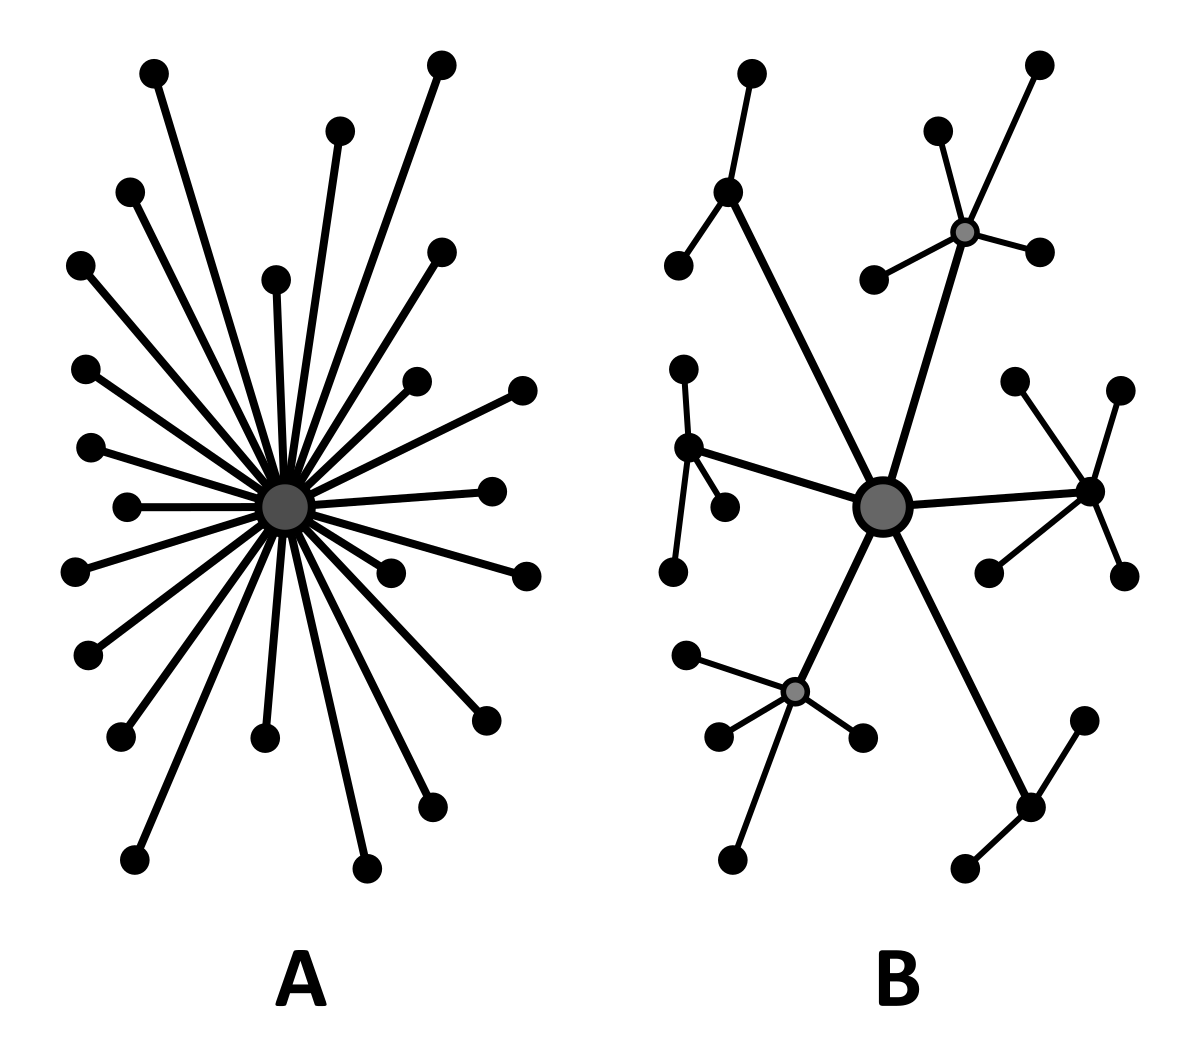
\includegraphics[height=8cm, width=8cm]{decentralization_diagram.png}
  \centering
  \caption{Topología de los distintos tipos de redes}
  \label{fig:topologia-tipo-redes}
\end{figure}

El gráfico A muestra un ejemplo de red totalmente centralizado en donde un solo nodo coordina o abastece el trabajo del resto de los participantes. En este caso, se puede notar claramente que si ese único nodo falla o, peor aún, es saboteado por un agente maligno, consecuentemente toda la red caerá o será controlada por dicho nodo central bajo potenciales efectos dañinos.

Por otro lado, el gráfico B muestra una arquitectura descentralizada mixta compuesta por varios cúmulos o \textit{clusters}. Si uno de los nodos responsables del control de un cúmulo es abordado malintencionadamente, el mismo se mantendrá fuera de control, pero dicha acción no afectará el curso total de la red.

Esta última característica es crucial para el presente trabajo puesto que la confianza ahora no dependerá solamente de un único punto sino de muchos otros, y esto, como se analizará posteriormente, disminuye exponencialmente la probabilidad de obtener todo el control de la red con el objeto de anunciar información espuria sobre ella.

\subsubsection{Historia de la descentralización}
\label{historia_descentralizacion}

Una de las primeras personas en investigar y proponer casos de uso concretos basándose en las ideas y las virtudes de la descentralización fue David Lee Chaum. En el año 1981 publicó un trabajo llamado \textit{Untraceable Electronic Mail, Return Addresses, and Digital Pseudonyms}\cite{Chaum1981} donde se brinda una solución al \textit{Problema del análisis de tráfico} el cual consiste en ocultar quién se comunica con quién y cuándo. Si bien en la época se habían desarrollado soluciones para este problema, la descrita en el trabajo de Chaum fue la primera en hacerlo de manera totalmente descentralizada, es decir, sin contar con los riesgos de tener que confiar en una autoridad central. Para ello, propone el uso de una red denominada \textit{Mix Network} en donde todos los nodos participantes son responsables de encriptar y desencriptar los mensajes en lotes paso a paso. El atractivo principal de este tipo de arquitectura para este problema es que si alguien con propósitos malévolos toma ilegítimamente el control de uno de los nodos (o incluso de varios), la red puede seguir garantizando su funcionamiento y su confiabilidad; en cambio, en una arquitectura con una autoridad central, cuando esta última es atacada y capturada, la confianza y la seguridad de toda la red queda totalmente comprometida porque el cumplimiento de estas propiedades depende precisamente de este nodo central.

En 1982 Chaum presentó su tesis doctoral titulada \textit{Computer Systems Established, Mantained and Trusted by Mutually Suspicius Group}\cite{Chaum1982} en donde se discute y se especifica formalmente la factibilidad y el diseño de un sistema genérico sobre el cual un conjunto de organizaciones no emparentadas entre si, es decir, sin requisitos de confianza mutua, puedan trabajar de forma segura y fiable mediante una ``caja fuerte'' (\textit{vault}). En dicho trabajo se explora exhaustivamente las técnicas de criptografía de clave pública, y respecto a la ``caja fuerte'', se demuestran las ventajas de disponer de muchas de ellas como forma de evitar el problema del único punto de falla.

En 1983 Chaum dio a conocer un nuevo artículo denominado \textit{Blind Signatures for Untraceable Payments}\cite{Chaum1983} en el cual se aborda específicamente, y por primera vez, la forma de realizar pagos -o transacciones de bienes- de manera anónima y segura. Se desarrolla para ello el concepto de firmas ciegas para disponer de autenticidad, trazabilidad y, al mismo tiempo, confidencialidad sobre los movimientos efectuados. Si bien este sistema propuesto no aborda la descentralización de las operaciones, en el mismo trabajo se menciona que dicha posibilidad podría ser plausible (tal como se demuestra en \cite{Chaum1982}) y se deja el terreno preparado para la introducción de un sistema transaccional completamente descentralizado.

\subsection{Recapitulación}
\label{recapitulacion_desc_problema}

En esta sección se ha presentado la idea de ``huella digital'' para archivos utilizando como herramienta matemática para tal fin a las funciones de una sola vía; se ha descrito el problema a tratar en este trabajo en donde no es conveniente publicar y gestionar dichas huellas en un servidor centralizado para evitar que la confiabilidad y la seguridad recaiga en único punto dentro de la arquitectura. A través de los distintos trabajos revelados a lo largo de la historia -y enunciados en este informe- se ha podido visualizar que la problemática de centralizar la información o, de manera equivalente, que la misma sea controlada por una autoridad central fue un punto a evitar y, consecuentemente, se han propuestos alternativas conceptuales -a nivel arquitectónico fundamentalmente- para eludir la cuestión del ``único punto de falla'' y obtener el control de todo un sistema por dicho medio.

Se puede establecer, como para concluir esta sección, que el uso de una arquitectura descentralizada robusta podría ofrecer claras ventajas, con miras a la fiabilidad y a la transparencia de las operaciones, respecto a una clásica arquitectura de un sólo servidor y muchos clientes para el problema que se ha planteado.

\newpage
\section{Marco teórico: blockchain}
\label{mt_blockchain}

En este capítulo se desarrollará todo el fundamento teórico relacionado a blockchain con el propósito de comprender las características y las propiedades de la solución propuesta para resolver el caso o problema descrito.

En primer lugar se hará una descripción contextualizada de los sucesos históricos más relevantes que propiciaron el desarrollo del concepto de blockchain tal como se conoce hoy en día. Cada uno de estos hitos brindará un aporte fundamental a la hora de entender más adelante los pilares de la blockchain. Posteriormente se presentará a Bitcoin, la primera implementación de blockchain exitosa, mostrando sus partes constitutivas y su funcionamiento como tal. Finalmente se desarrollará Ethereum, la blockchain que se usará para el desarrollo de la solución al problema tratado en este trabajo, desde un punto de vista comparativo a Bitcoin y con el agregado de los contratos inteligentes, pieza clave para la resolución descentralizada y trazable de problemas -en particular, nuevamente, el detallado en esta tesina-.

\subsection{Orígenes}

Antes de comenzar con los conceptos teóricos en torno a de blockchain, se hará un repaso de los sucesos históricos que ayudaron o influyeron en la constitución de esta idea como tal. La necesidad de hacer esto se fundamenta en dos razones: en primer lugar, seguir con la línea histórica introducida en el capítulo anterior dentro del marco de los fundamentos que se analizarán en este apartado. Y en segundo lugar, porque se verá que la culminación de la noción de blockchain reviste otras ideas relacionadas que se fueron gestando con anterioridad. Consecuentemente, se tratará de explicar las más importantes en orden histórico antes de llegar a la representación final de blockchain.

\subsubsection{Primer prototipo de cadena de bloques (blockchain)}
\label{bc_origins_blockchain}

En el año 1991, los científicos Stuart Haber y W. Scott Stornetta publicaron un artículo denominado \textit{How to Time-Stamp a Digital Document \cite{Haber:1991:TDD:2724969.2725089}} (``¿Cómo asignarle una fecha/hora a un documento digital?'' sería la traducción aproximada) en donde se analiza un problema similar al presentado en esta tesina. Se podría decir, básicamente, que la idea en común es poder verificar la inmutabilidad de un recurso digital desde un determinado momento. Dentro del contexto del trabajo recientemente citado, en donde el objetivo concreto es encontrar un mecanismo para sellar documentos digitales en el tiempo de manera tal que sea prácticamente incorruptible, se desarrollan dos tipos de soluciones, una centralizada y otra distribuida. Más allá de los detalles de implementación de ambas solución -en donde, como dato anecdótico, es interesante notar que la opción distribuida se titula como ``confianza distribuida'' en dicho artículo-, lo que sea desea recalcar y puntualizar de dicho trabajo es la idea de enlazar las certificaciones, es decir, el acto de informar que un archivo tiene determinado contenido (a través de la huella digital) a partir de una fecha y hora concreta, unas con otras de manera tal de incluir fragmentos de certificaciones previas en la certificación actual. Formalmente, esto sería:

\begin{equation}
  C_n = (n, t_n, ID_n, y_n, L_n)
\end{equation}

donde $C_n$, la certificación en sí, es una tupla compuesta por su número de secuencia $n$, el \textit{timestamp} $t_n$, el identificador del cliente $ID_n$, o sea, quien hace la petición de certificación, la huella digital $y_n$ del documento a certificar y $L_n$ es una porción de datos de la certificación previa:

\begin{equation}
  L_n = (t_{n-1}, ID_{n-1}, y_{n-1}, H(L_{n-1}))
\end{equation}

donde tanto el \textit{timestamp} como el identificador del cliente y la huella digital provienen de la certificación inmediatamente predecesora y, junto a esto, se incluye una huella digital ($H$ es una función de hash) de una porción de datos previa, es decir, de datos de la certificación $C_{n-2}$

A continuación se muestra un gráfico ilustrativo sobre la cadena de certificación que se formaría, extraída de \cite{Narayanan:2016:BCT:2994437}

\begin{figure}[H]
  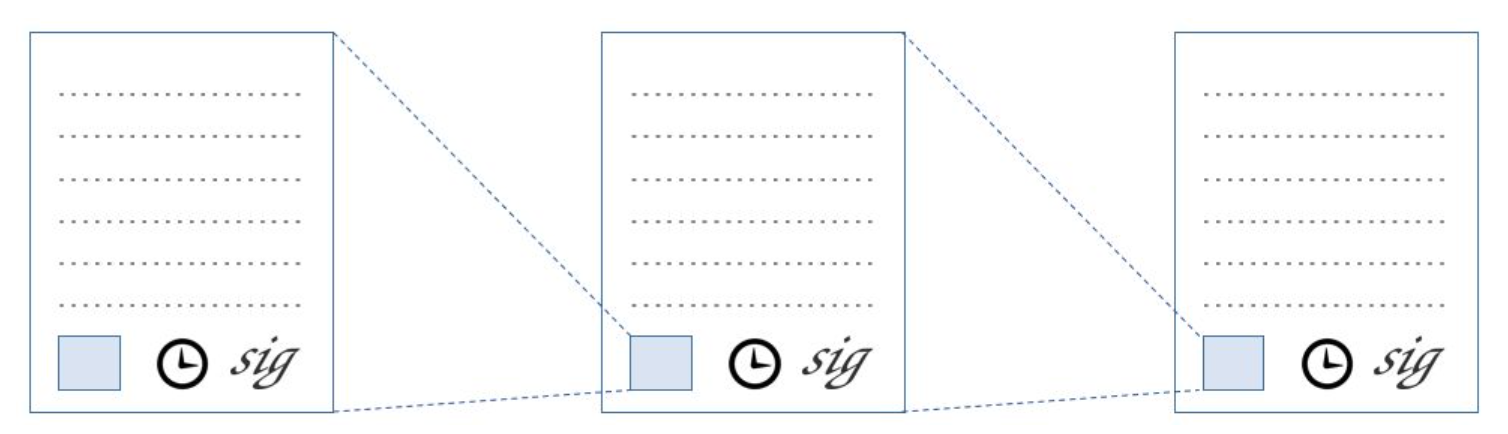
\includegraphics[height=6cm, width=14cm]{timestamps_chain.png}
  \centering
  \caption{Cadena de \textit{timestamps}  }
  \label{fig:timestamps-chain}
\end{figure}

La consecuencia más importante de lo expuesto en el trabajo presentado por Haber y Stornetta es que si, por ejemplo, por alguna razón se altera la huella digital de la certificación $C_i$, $y_i$, entonces el resto de las $k$ certificaciones subsiguientes quedarán corruptas ya que si:

\begin{equation}
  C_i = (i, t_i, ID_i, y_i; L_i)
\end{equation}

Y al analizar la $k$ certificacion siguiente a $C_i$, es decir, $C_{i+k}$:

\begin{align}
  C_{i+k}     &= (i+k, t_{i+k}, ID_{i+k}, y_{i+k}, L_{i+k})\\
  L_{i+k}     &= (t_{i+k-1}, ID_{i+k-1}, y_{i+k-1}, H(L_{i+k-1}))\\
  L_{i+k-1}   &= (t_{i+k-2}, ID_{i+k-2}, y_{i+k-2}, H(L_{i+k-2}))\\
  \dots\\
  L_{i+k-k+1} &= L_{i+1} = (t_i, ID_i, y_i, H(L_i))
\end{align}

Se puede ver como toda la secuencia $i+k$ hasta llegar a $i+1$ se referencian hacia atrás a través de una huella computada por la función $H$. En el caso particular de $L_{i+1}$, la huella $H$ de la tupla correspondiente, es decir, $(t_i, ID_i, y_i, H(L_{i+1}))$ será totalmente distinta si el valor de $y_i$ fue alterado y, desde ese punto hacia delante, el resto de las certificaciones quedarán inválidas porque la referencia hacia atrás de la huella cambiará completamente. Es decir, si la alteración se expresa como $y_i'$, entonces:

\begin{align}
  L_{i+k-k+1}' &= L_{i+1}' = (t_i, ID_i, y_i', H(L_i))\\
  L_{i+k-k+2}' &= L_{i+2}' = (t_{i+1}, ID_{i+1}, y_{i+1}, H(L_{i+1}'))\\
  \dots\\
  L_{i+k}'     &= (t_{i+k-1}, ID_{i+k-1}, y_{i+k-1}, H(L_{i+k-1}'))
\end{align}

Las ecuaciones previas muestran cómo la cadena de referencias entre certificaciones conectadas diverge cuando uno de los ``eslabones'' cambia su contenido. Siguiendo estos procedimientos, es fácilmente verificable cuándo y dónde una certificación fue alterada y, por esta razón, este enlazamiento es resistente a los cambios que se produzcan, se deban a razones fortuitas o malintencionadas.

Desde el punto de vista histórico, este representa el primer trabajo en donde se utiliza una \textit{cadena de bloques (blockchain)} como estructura de datos principal para el almacenamiento con detección y/o protección de cambios. Entender estos conceptos servirá luego para comprender mejor cómo las implementaciones contemporáneas de las diversas blockchains funcionan hoy en día dado que es, probablemente, el núcleo lógico de este tipo de arquitecturas o redes.

\subsubsection{Mejora del prototipo: inclusión de árbol de Merkle}
\label{bc_origins_merkle}

Dos años después de la publicación \textit{How to Time-Stamp a Digital Document \cite{Haber:1991:TDD:2724969.2725089}}, es decir, en 1993, los mismos autores del artículo original junto a Dave Bayer publican uno nuevo denominado \textit{Improving the Efficiency and Reliability of Digital Time-Stamping \cite{BayerHaberStornetta1993}} (traducido aproximadamente a ``Mejorando la eficiencia y la confianza de un servicio digital de sellado de tiempo''). La idea de esta revisión es agregar una alternativa más con el propósito de mejorar la eficiencia a la hora de almacenar y verificar las certificaciones, a cambio de relajar un poco la precisión de estos sellados: en lugar de enlazar y sellar cada certificación, el nuevo mecanismo presentado propone mantener una cadena maestra donde cada uno de los eslabones mantiene la integridad de un grupo o bloque de certificaciones que se emitieron en un determinado lapso de tiempo. Se verá a continuación un gráfico extraído de \cite{Narayanan:2016:BCT:2994437} ilustrando la idea explicada recientemente:

\begin{figure}[H]
  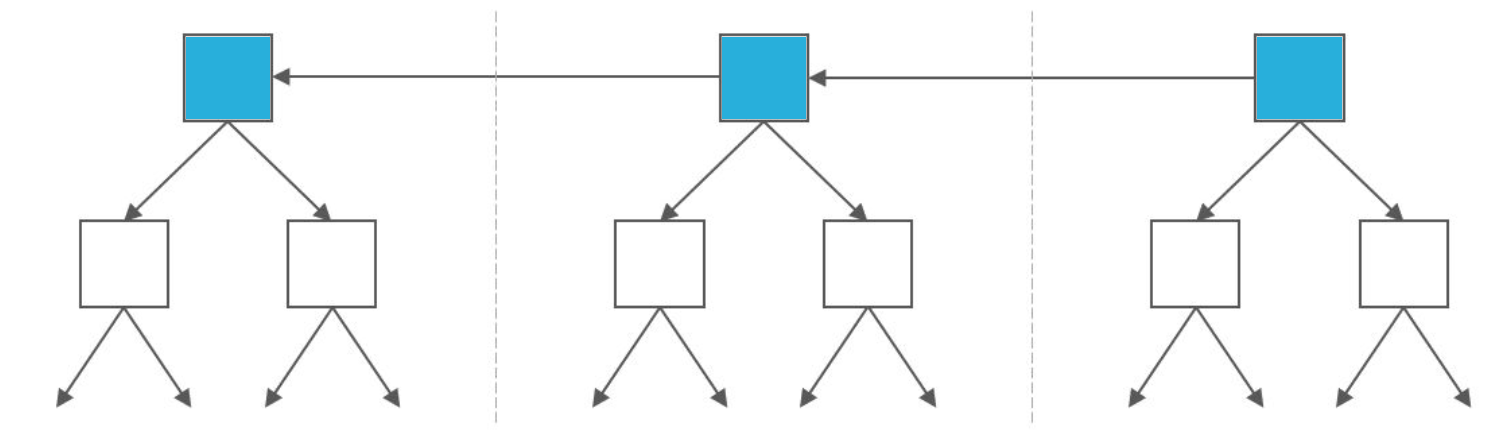
\includegraphics[height=6cm, width=14cm]{tree_timestamps_chain.png}
  \centering
  \caption{Cadena de \textit{timestamps} arbolada }
  \label{fig:tree-timestamps-chain}
\end{figure}

Los bloques sombreados son parte de la cadena maestra y cada eslabón agrupa una determinada cantidad de certificaciones en un periodo de tiempo esquematizado a través de la línea punteada. Lo importante de destacar es que, desde la perspectiva de quien o quienes mantienen la cadena maestra, cada agrupamiento, representado por cada uno de los eslabones, no almacena la partición completa de los certificados asignados sino que mantiene tan sólo la huella de la raíz del \textit{árbol de Merkle} de todos ellos. Dicha estructura, caracterizada y explicada por Ralph Merkle (de ahí el nombre) en \cite{Merkle1980} para un artículo de sistemas criptográficos, es un árbol binario donde los nodos hoja representan el dato de interés más su huella digital y cada nodo interno es, recursivamente, la huella digital de la huellas ``Merkle'' concatenadas de cada uno de los subárboles. Formalmente sería algo como:

\begin{equation}
  MT_{val}(t) = \begin{cases*}
   h(data(t))  & si t es hoja\\
   h(MT_{val}(sa_{izq}(t)) + MT_{val}(sa_{der}(t)))  & si t es interno
        \end{cases*}
\end{equation}

donde $t$ es un nodo, $h$ es una función de \textit{hash}, $data$ es una función que obtiene el dato de interés a partir de un nodo, $sa_{izq}$ y $sa_{der}$ son funciones que denotan el subárbol izquierdo y derecho, respectivamente, a partir de un nodo y $+$ es una operación de concatenación similar a la homónima para \textit{strings}.

A fin de comprender mejor el concepto, a continuación se revelará un ejemplo gráfico:

\begin{figure}[H]
  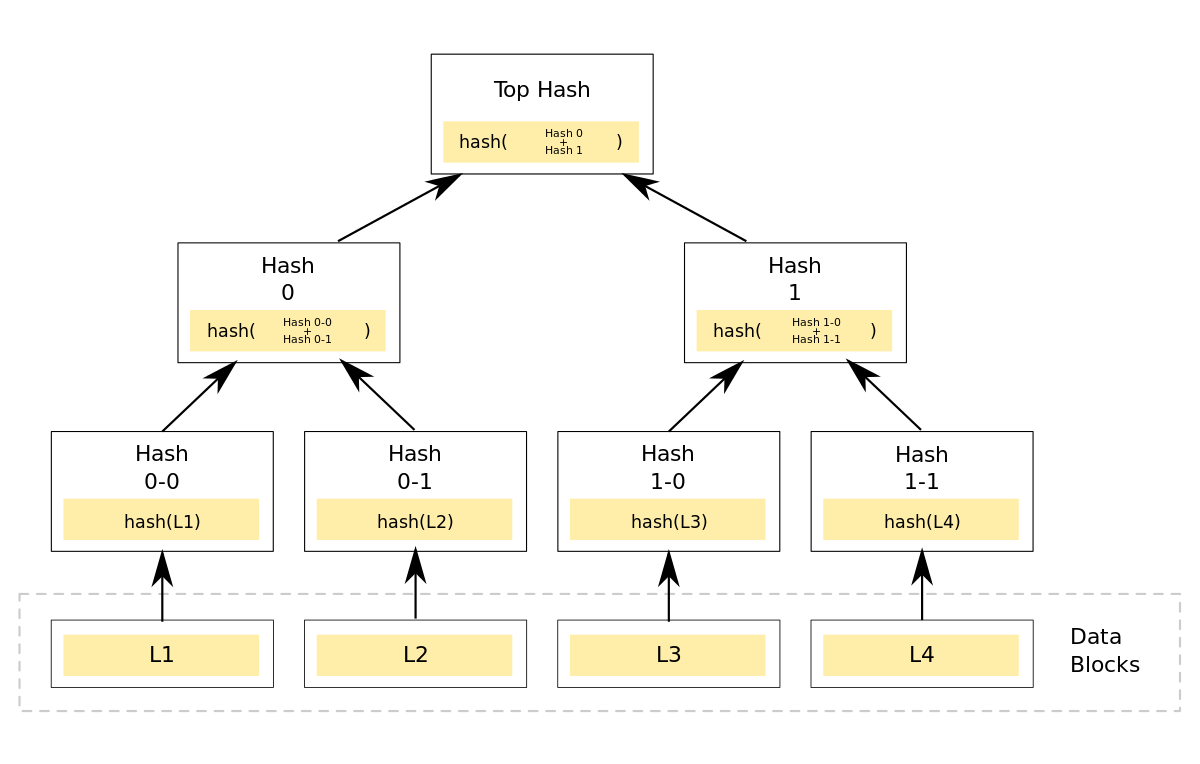
\includegraphics[height=10cm, width=14cm]{merkle_tree_example.png}
  \centering
  \caption{Ejemplo de árbol de Merkle }
  \label{fig:merkle-tree-example}
\end{figure}

Se muestra claramente en la figura anterior como el nodo raíz mantiene la huella de sus nodos hijos, y así, recursivamente, hasta llegar a los nodos hoja que contienen o apuntan directamente a los datos concretos.

Retomando el contexto previo, el de la cadena maestra del artículo \cite{BayerHaberStornetta1993}, donde se ha establecido que cada eslabón es una raíz \textit{Merkle} de un conjunto de certificaciones en un lapso de tiempo, se presentan, al menos, dos ventajas destacables:

\begin{enumerate}
  \item La cadena maestra, tal como se insinuó anteriormente, no requiere de todas las certificaciones. Hay que puntualizar que un eslabón ya no es más la representación de una simple certificación, sino que más bien sería el resumen -por medio de una huella digital- de un bloque de certificaciones, donde cada una de ellas posiblemente esté ubicada en otros lugares físicos.

    Tal como se explica en el artículo de Bayer, Haber y Stornetta, la idea es distribuir el gobierno de los distintos subárboles que componen un eslabón en diferentes partes de la red y promover las huellas hacia arriba, es decir, hacia la cadena maestra como si fuera un torneo eliminatorio de un juego 1 vs 1. El objetivo de esto es reducir el espacio insumido en mantener certificaciones en los puntos de validación sólo para tal fin.
  \item Relacionado al punto anterior, con esta nueva disposición no se necesitan revisar N certificados para legitimar la integridad de uno particular, sino que ahora se requieren $\log_2 N$ verificaciones mejorando enormemente los tiempos para realizar dicha tarea. Por ejemplo, en base a la figura \ref{fig:merkle-tree-example} -que cuenta con cuatro datos concretos-, si se deseara verificar la integridad de \textit{L4}, se debería obtener la huella de este dato -\textit{Hash 1-1}-  y, adicionalmente, tener disponibles las huellas de \textit{Hash 1-0} y de \textit{Hash 0}: con la primera y la segunda se obtendría \textit{Hash 1} y con esta última más la tercera, es decir, \textit{Hash 0}, se obtendría la raíz Merkle a comparar contra la registrada en la cadena maestra, dando un total de 3 verificaciones, es decir, $O(\log_2 N)$ (con 8 certificaciones se necesitarían 4 verificaciones, con 16, 5, y así sucesivamente).
\end{enumerate}

En definitiva, esta ampliación \cite{BayerHaberStornetta1993} del trabajo original \cite{Haber:1991:TDD:2724969.2725089} presenta mejoras, respecto a la cadena de bloques esbozada originalmente, desde el punto de vista de la eficiencia en espacio y tiempo, y se aproxima aun más a las implementaciones recientes de lo que se conoce como blockchain. Tal como se verá más adelante, estas nociones estarán muy presentes al momento de estudiar las bases de dichas estructuras.

\subsubsection{Hashcash: primer servicio en usar Prueba-de-Trabajo}
\label{bc_origins_hashcash}

En esta subsección se explicará uno de los últimos pilares necesarios para entender de manera integral el funcionamiento de blockchain tal como se conoce en estos tiempos. Para ello, y continuando con la línea histórica, se expondrá una solución a un problema que a simple vista no está para nada emparentado con la clase de problemas que trata blockchain, pero que sin embargo, tuvo un enorme impacto e influencia en una parte fundamental del objeto de estudio de este capítulo.

Ya en la década de 1990, en pleno auge de Internet, uno de los principales problemas surgido en aquel entonces era el del correo basura o \textit{spam}, denominado así al correo enviado masiva e indiscriminadamente con propósitos publicitarios o malintencionados. Desde entonces se han diseñado una vasta cantidad de estrategias y filtros anti-spam de diversa índole para evitar esta clase de correos.

Uno de esos mecanismos surgió a partir de una idea de un criptógrafo inglés conocido como Adam Back, pensado e implementado en mayo de 1997 y publicado formalmente en agosto de 2002, al cual bautizó como Hashcash \cite{Back2002}. El principal argumento detrás de este método antispam es el siguiente: alguien interesado en enviar un correo no tendrá mayores problemas en demorar unos segundos la salida del mismo, pero en cambio, sumar esta demora en cada uno de los masivos correos salientes por parte de un cliente de \textit{spam}, hará que su negocio sea inviable, y forzosamente, tendrá que desistir de ello. Ahora bien, esa demora no puede ser cualquier demora, pues de lo contrario, sería fácilmente evitable por el emisor. Tendría que poseer la propiedad de ser verificable trivialmente por un tercero -que tranquilamente podría ser el receptor- de manera tal de poder demostrar fehacientemente que el emisor dedicó un esfuerzo o un trabajo para enviar dicho correo al remitente deseado, y de esta manera, cerciorarse que existió un interés real en realizar dicha acción. En síntesis, se requiere de un método en donde sea fácil y rápido de demostrar por un receptor que el emisor invirtió un tiempo moderado en el envío del correo.

La propuesta técnica presentada en el trabajo de Adam Back para cumplir con los requisitos presentados en el párrafo anterior consiste en describir una familia de funciones \textit{costo} de la siguiente forma:

\begin{equation} \label{eq:funciones-costo}
  \begin{cases*}
    T \leftarrow Mint(s, w)\\
    V \leftarrow Value(T)
  \end{cases*}
\end{equation}

$Mint$ es el procedimiento que realiza la inversión de trabajo a través de un desafio computacional con una serie de metadatos $s$ y una dificultad de trabajo $w$ que debería ajustarse de alguna forma para que siempre sea moderada de acuerdo al poder de cómputo físico disponible. El resultado de esto se traduce a un \textit{token} $T$. Por otra parte, $Value$ es la función que verifica velozmente que el \textit{token} $T$ es válido, demostrando de esta manera que hubo trabajo real al momento de computar este \textit{token}.

Las propiedades que deben cumplirse para esta familia de funciones son:

\begin{itemize}
  \item Como se ha dejado expresado, $Mint$ debe ser una función de costo de cómputo moderado mientras que $Value$ deberá computarse trivialmente.
  \item Ser públicamente auditables, es decir, que se conozca perfectamente su funcionamiento.
  \item Tener costo fijo o probabilístico, es decir, que el costo dedicado a la inversión de esfuerzo sea fijo, o bien, probabilísticamente predecible y/o regular en la práctica.
  \item No disponer de ningún mecanismo para realizar inversiones de trabajo de manera fácil. Esto se exige para no ofrecer ninguna clase de ventaja a ciertos usuarios.
\end{itemize}

Cabe destacar que la función que usa Hashcash cumple con todas las precondiciones presentadas. Antes de presentar su descripción formal, conviene explicar brevemente y de manera simplificada su funcionamiento dentro del contexto en la cual fue desarrollada, es decir, en los correos electrónicos \cite{Adam2006}.

El emisor deberá realizar el siguiente procedimiento:

\begin{enumerate}
\item Se construye una cadena $s$ de la forma:
\begin{equation}
fecha:remitente:contador
\end{equation}
Por ejemplo:
\begin{equation}
  20190118190000:xyz@abc.com:00000000
\end{equation}
\item Se computa una huella digital $h$ de la cadena $s$ por medio de una función de hash $H$.
  \begin{enumerate}
    \item Si los primeros $k$ digitos de $h$ son 0 ($k$ es un párametro que depende directamente de la dificultad del desafío), entonces se ha encontrado el \textit{token} $T$ del esfuerzo invertido. La cadena $s$ se adjunta en una cabecera especial del correo (\textit{X-Hashcash}) al momento de enviarse.
    \item Si no, se incrementa en una unidad la parte del contador de la cadena $s$ y se vuelve a repetir el procedimiento a partir del segundo paso.
  \end{enumerate}
\end{enumerate}

Luego, el receptor deberá proceder así:

\begin{enumerate}
  \item Se extrae de la cabecera del correo electrónico la cadena $s$ adjuntada (\textit{X-Hashcash})
  \item Se computa una huella digital $h$ de la cadena $s$ por medio de una función de hash $H$.
  \begin{enumerate}
    \item Si $h$ cumple con el desafío, es decir, la cantidad inicial de $k$ digitos 0 preestablecida, entonces, el correo pasa el filtro.
    \item De lo contrario, el correo se descarta por no validar el desafío impuesto.
  \end{enumerate}
\end{enumerate}

Y formalmente, la función presenta esta forma, comparable a la ecuación \ref{eq:funciones-costo}:

\begin{equation}
  \begin{cases*}
    T \leftarrow Mint(s, w), \mathbf{hallar}\; x \in \{0, 1\}^*\; \mathbf{tq}\; H(s+t) \propto_w 0^k \\
    V \leftarrow Value(T),  \mathbf{verificar}\; H(s+t) \propto_w 0^k
  \end{cases*}
\end{equation}

donde la semántica de todas las variables coincide con lo explicado en los procedimientos precedentes, a excepción del operador $\propto_w$ cuyo significado sería: ``los $k$ primeros dígitos de la cadena de la izquierda tienen que coincidir completamente con la cadena de la derecha''.

En resumen, la implementación y el artículo posterior de Adam Back presenta una técnica para verificar rápidamente el trabajo exigido -con un esfuerzo considerable- a través de un desafío computacional, de un participante de una red, con el objeto de garantizar que éste tiene genuino interés en realizar determinada tarea (enviar un correo electrónico, en el caso particular del trabajo de Adam Back).

Este sistema fue el primer caso popular y documentado -con un precursor similar tratado en \cite{Dwork1992}- de un algoritmo de Prueba-de-Trabajo -formalizado y nombrado en \cite{Jakobsson1999}-. Luego se estudiará en detalle y se verá que es vital en el funcionamiento de blockchain.

\subsubsection{B-money y Bit gold: primeros precursores monetarios de Bitcoin}
\label{bc_origins_bmbg}

Aproximadamente una década antes de la publicación del \textit{paper} de Bitcoin -y de su blockchain-, se describieron bocetos y propuestas informales que pretendían como objetivo lograr la descentralización -cuanto menos- de los sistemas monetarios.

En 1998, un estudiante de computación y aficionado a la criptoanarquía conocido como Wei Dai, publica en las listas de correo de aquel entonces un ensayo titulado \textit{bmoney}\cite{Narayanan:2016:BCT:2994437}\cite{WeiDai1998} en donde propone y detalla resumidamente cómo debería implementarse una moneda prescindiendo de una entidad central que controle la creación y el curso de las mismas. En su lugar, se plantea el uso de un método de Prueba-de-Trabajo, similar al repasado previamente en Hashcash, para la creación de monedas: se presenta un desafío computacional y quien lo resuelva -tras un arduo esfuerzo- recibe una recompensa por ello. Para la transferencia de activos, Dai plantea que cada participante de la red -identificado por una clave pública-, o bien, un subconjunto de ellos, mantenga la información de toda la red, en particular, del balance corriente de todas las cuentas de los usuarios, y que todos sean capaces de enviar y recibir mensajes -firmados con una clave privada-  a o hacia todos para mantener actualizado el estado global de toda la red en conjunto, correspondiéndose este comportamiento al de un sistema totalmente distribuido. Asimismo, se manifiesta también dentro del protocolo esbozado, la idea de ``contratos'', es decir, de acuerdos entre dos partes de la red arbitrado por una tercera, con un pseudo esquema de penalizaciones y consenso en los casos de incumplimiento o desacuerdo.

En el mismo año -1998- un científico de la computación llamado Nick Szabo propone una idea similar a la cual bautiza como \textit{Bit Gold}\cite{Narayanan:2016:BCT:2994437}\cite{Szabo1998}. En él, la propuesta básica es también usar un método de Prueba-de-Trabajo a partir de un desafío para la generación de monedas, y la solución de este problema sumado al uso de sellado distribuido de tiempo y el enlazado de todas ellas en una cadena global y distribuida conformarían el protocolo.

Ambas propuestas son bastantes laxas y carecen de la formalidad y la robustez de un trabajo de investigación o \textit{paper}. Sin embargo, han sentado precedentes históricos en cuanto al desarrollo y a la consolidación del concepto contemporáneo de blockchain. Entre ellas:

\begin{itemize}
  \item La idea aproximada de distribuir el estado global de la red entre los distintos participantes de la misma, o sobre un subconjunto de ellos.
  \item El uso de Prueba-de-Trabajo. Si bien se verá que en las blockchains más modernas no se utiliza para el ``acuñamiento'' de criptomonedas, termina siendo parte sustancial de la solución en otros aspectos.
  \item El uso de criptografía asimétrica -clave pública y privada- para identificar la propiedad de las transacciones.
  \item El concepto de ``contratos'': \textit{B-Money} brinda una explicación informal sobre esto y Nick Szabo desarrolla una propuesta formal en \cite{Szabo1997} sobre la idea que, años más tarde, se convertiría en el eje central de la blockchain de Ethereum \cite{Buterin2014}, a explicarse durante el desarrollo de este capítulo.
\end{itemize}


\subsection{Bitcoin: primera implementación de blockchain}

En esta subsección se describirá Bitcoin, y más específicamente, la blockchain que le da sentido y sustento tecnológico a dicha criptomoneda. A lo largo de este apartado se verá cómo los temas desarrollados previamente tendrán su impacto en la formulación de la idea de blockchain. Dicho en otros términos, se apuntará a describir el \textit{paper} seminal de Bitcoin como una composición y conjugación de los temas recientemente vistos y no como un trabajo totalmente aislado de su contexto histórico.

\subsubsection{Historia}

En 2008, Satoshi Nakamoto -un pseudónimo para una persona o grupo de personas desconocidas- publica en las listas de correo un \textit{paper} titulado \textit{Bitcoin: A Peer-to-Peer Electronic Cash System} (traducido aproximadamente a ``Bitcoin: un sistema de efectivo electrónico usuario-a-usuario''), el cual describe un sistema de pago electrónico distribuido, independiente de terceras entidades requeridas para el control y el curso válido de la moneda. A diferencia de las propuestas previas presentadas aproximadamente una década atrás por Wei Dai y Nick Szabo, este artículo describe con suficiente rigurosidad y completitud todos los aspectos necesarios para que el sistema monetario presentado funcione de forma confiable.

En 2009 se puso en marcha la red Bitcoin por medio de una implementación inicial provista por el mismo Satoshi Nakamoto y, desde entonces, ha crecido significativamente de la mano de muchos programadores alrededor del mundo. Satoshi, por su parte, dejó el desarrollo en el año 2011 y su presencia y participación en las redes se ha desvanecido por completo.

Más allá de que su futuro en la economía y en las finanzas es revolucionario y, al mismo tiempo, incierto, también fue igualmente revolucionaria la infraestructura detrás del Bitcoin, es decir, la blockchain, que a partir de este puntapié inicial abriría el terreno para presentar esta tecnología a muchos otros dominios, amén de las criptomonedas.

\subsubsection{Componentes de la blockchain}
\label{bc_bitcoin_components}

En esta sección se describirán las partes constitutivas de la blockchain de Bitcoin que, fundamentalmente, son dos: por un lado los bloques -conectados entre sí formando la típica cadena de bloques- y por otro lado las transacciones, las cuales en conjunto conforman a los bloques.

\paragraph{Transacción}
\label{bc_bitcoin_transaction}

Las transacciones son las unidades constitutivas de la blockchain de Bitcoin. Denotan de cierta manera la propiedad de un recurso que, para el caso particular de Bitcoin, se trata de un valor monetario intangible.

A continuación se mostrará el primer gráfico de una cadena de transacciones, extraído del \textit{paper} de Nakamoto:

\begin{figure}[H]
  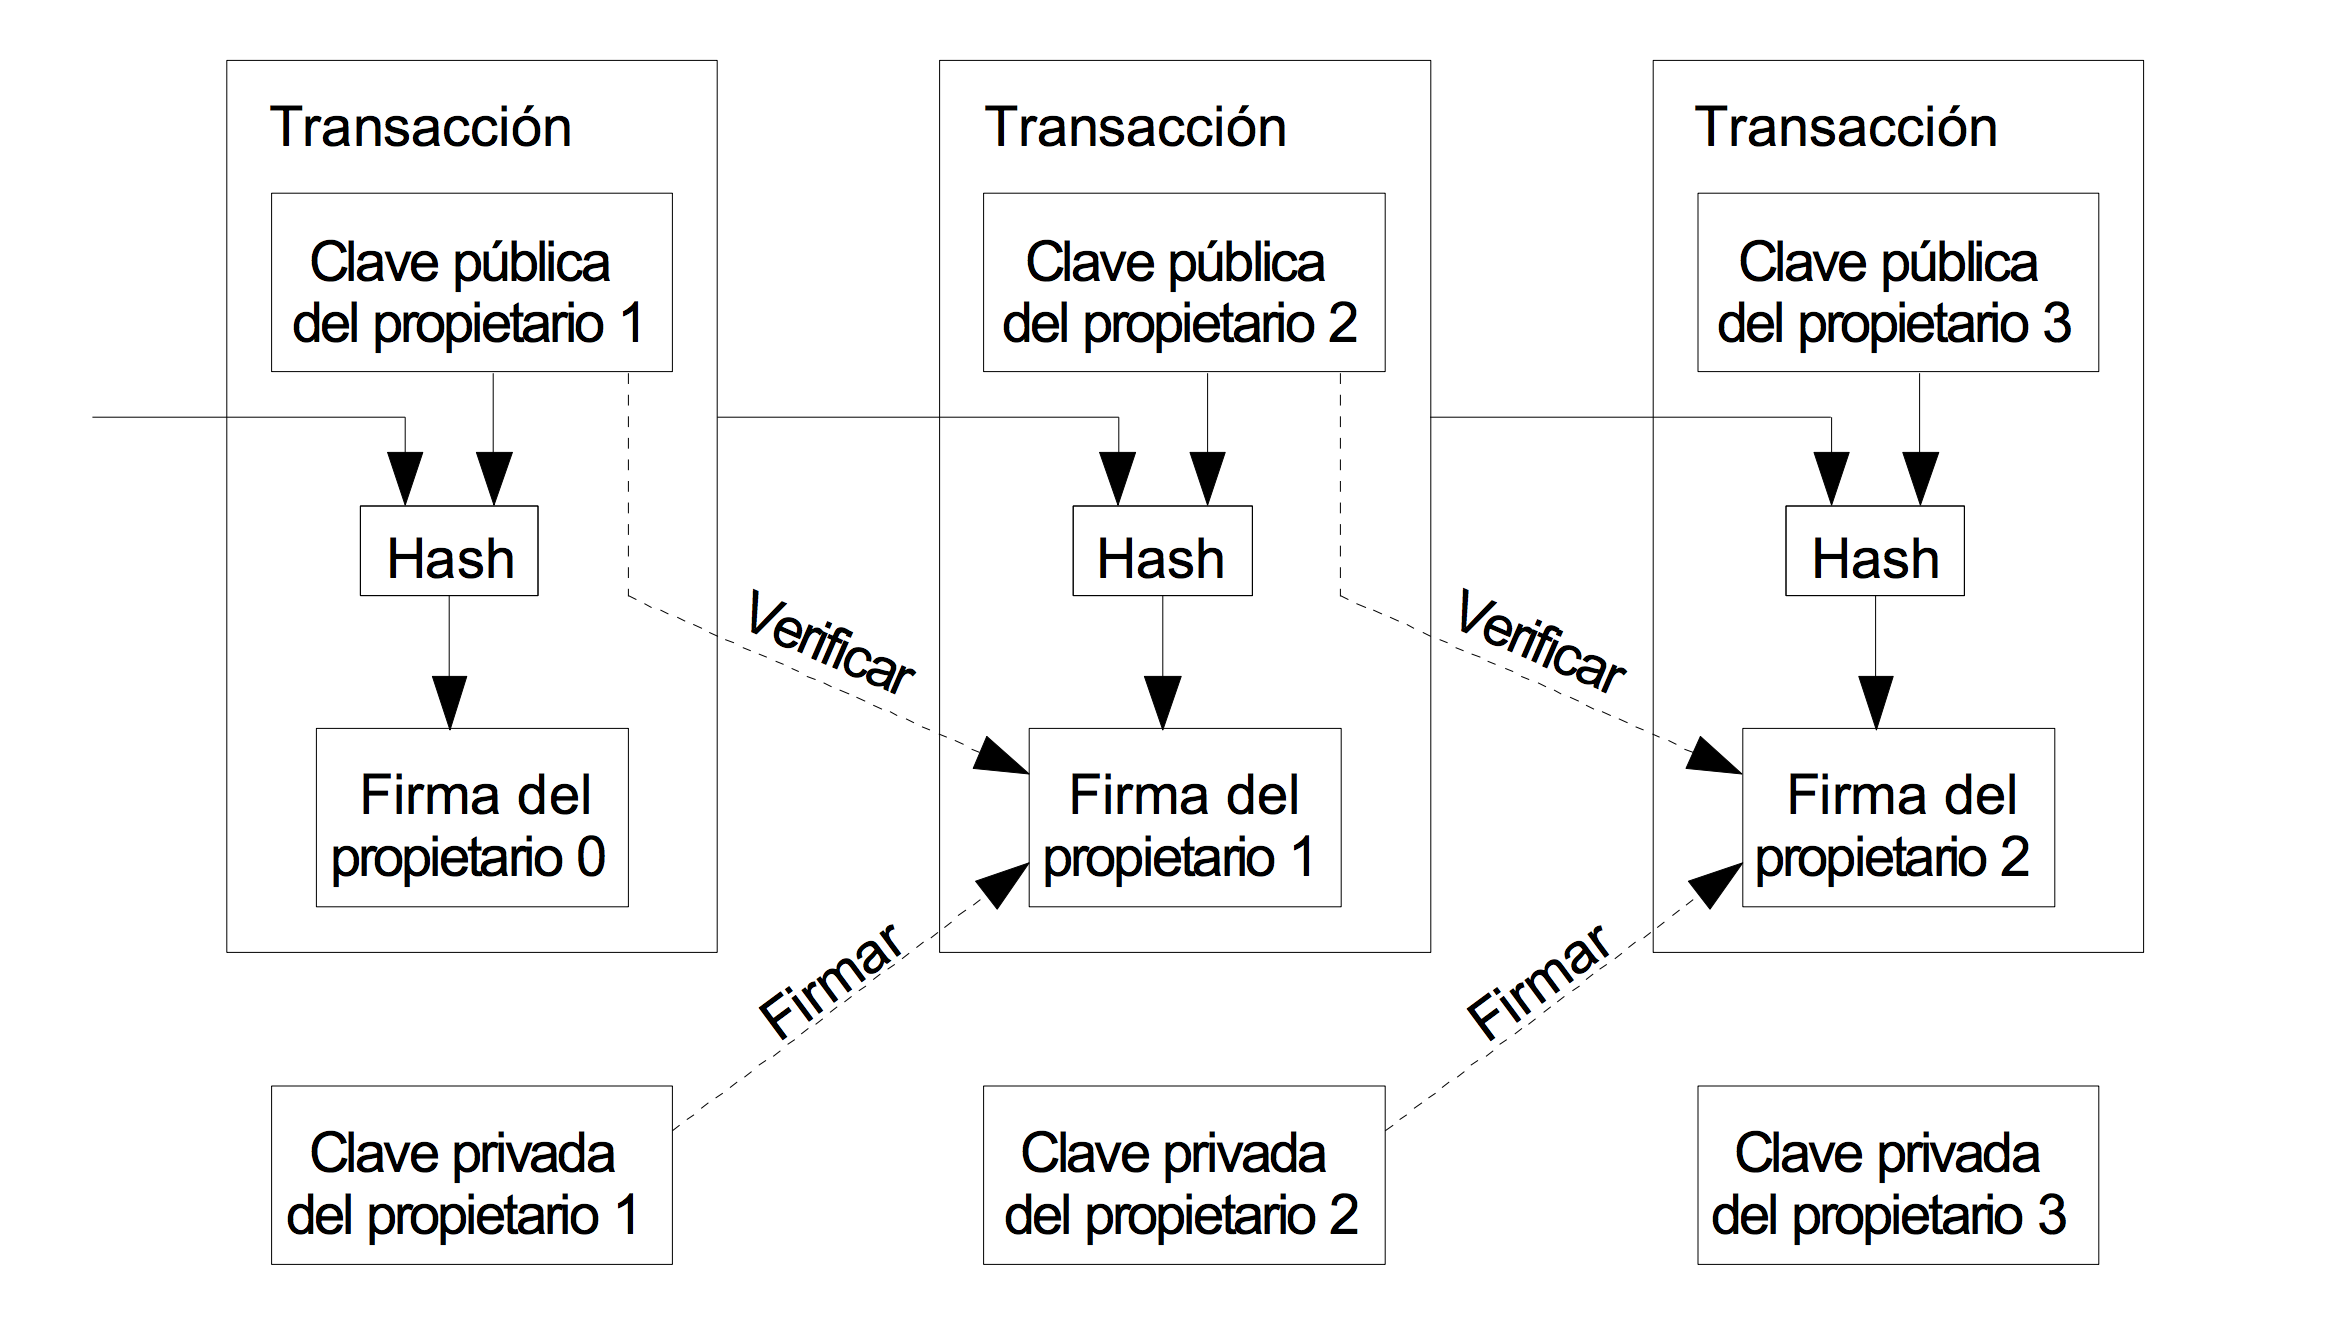
\includegraphics[height=8.5cm, width=14cm]{bitcoin_transaction_paper.png}
  \centering
  \caption{Cadena de transacciones, de Satoshi Nakamoto}
  \label{fig:bitcoin-transaction-paper}
\end{figure}

Es importante destacar, antes de puntualizar algunos aspectos del gráfico, que esta representación no ejemplifica fielmente la implementación real de una transacción en Bitcoin, pero es útil como primera aproximación y se verá posteriormente un modelo muchísimo más cercano al real.

Ahora sí, volviendo a la figura \ref{fig:bitcoin-transaction-paper} se puede tomar nota de lo siguiente:

\begin{itemize}
  \item Las transacciones están enlazadas en serie, formando una cadena de propiedad.
  \item El recurso $r$ asociado a la transacción en la posición $i$ de la cadena corresponde a un propietario $x$.
  \item El recurso $r$, ya sea de forma total o parcial, provenía de la transacción $i - 1$ donde el propietario era $y$.
  \item A través de criptografía asimétrica se usa una clave privada para firmar y autorizar una acción, y con la clave pública asociada se puede verificar que dicha firma es auténtica, es decir, que corresponde a quien efectivamente la ejecutó.
  \item En el contexto de las transacciones, se usa la clave privada para firmar una nueva transacción representando el pase de un recurso a otro propietario. A través de la clave pública asociada, cualquiera puede constatar que dicha transacción, y por ende dicho pase, fue autorizado por el propietario anterior. Por ejemplo, la transacción $i$ fue firmada por el propietario $y$ autorizando la transferencia de su recurso al propietario $x$ y referenciando la anterior propiedad de su propio recurso proveniente de la transacción $i - 1$.
\end{itemize}

Cabe recalcar en este punto que todas las transacciones son públicas, o dicho en otras palabras, se difunden por toda la red. Y otra cuestión importante que vale la pena aclarar es que las transacciones son los únicos elementos que describen la propiedad de los recursos dentro de la red. Esto significa que no existen ni cuentas, ni balances, ni usuarios; únicamente existen transacciones que podrán estar o no ``gastadas'' -concepto que se aclarará luego-.

A continuación se hará una descripción más verosímil de la estructura de una transacción en Bitcoin. En primer lugar, el siguiente gráfico ayudará a visualizar un poco mejor cómo es realmente la cadena de transacciones comparada a la anterior de la figura \ref{fig:bitcoin-transaction-paper}:

\begin{figure}[H]
  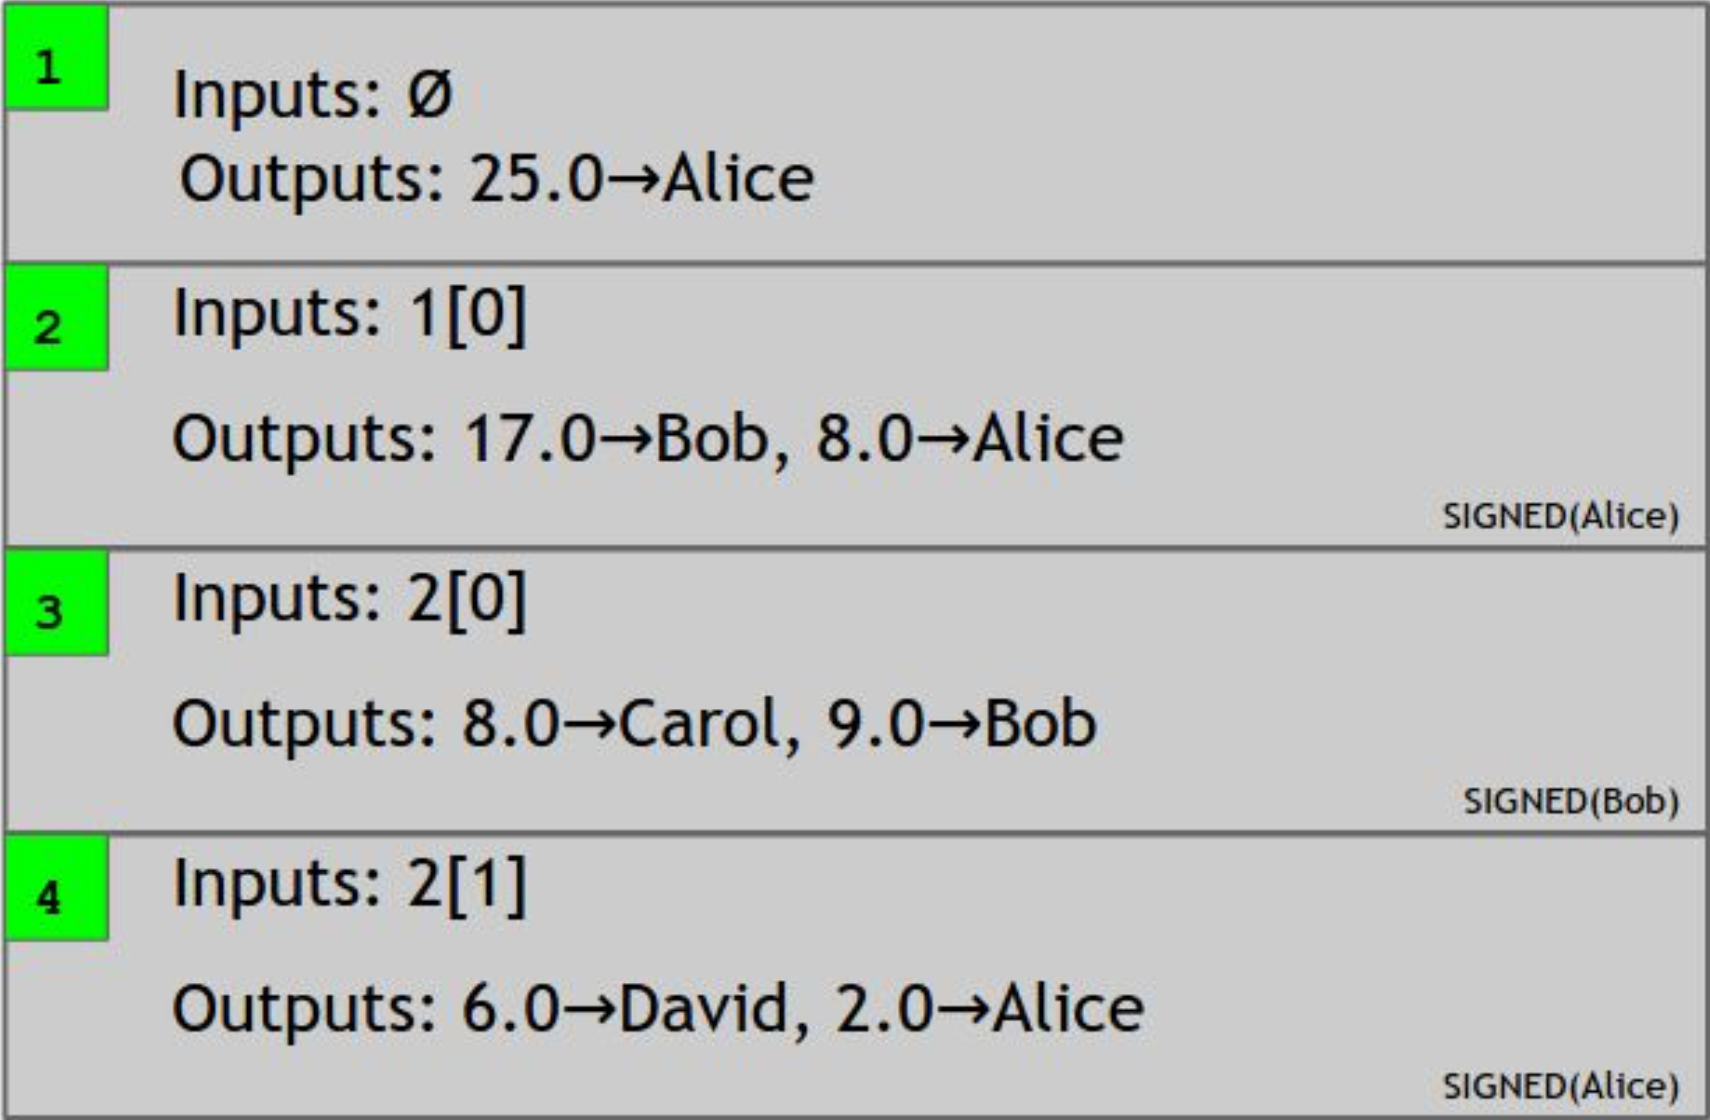
\includegraphics[height=8cm, width=12cm]{bitcoin_transaction_bitcoincore.png}
  \centering
  \caption{Cadena de transacciones, muy similar a Bitcoin (gráfico extraído de \cite{Narayanan:2016:BCT:2994437})}
  \label{fig:bitcoin-transaction-bitcoincore}
\end{figure}

El cambio más significativo respecto a lo explicado anteriormente es que las transacciones, en realidad, poseen entradas y salidas -\textit{inputs} y \textit{outputs}, respectivamente-. Una entrada es una referencia a una salida de una transacción previa, mientras que una salida es un valor o recurso a transferir junto a algo similar a la dirección del beneficiario (no es exacta esta descripción, pero se detallará más adelante). Es decir que dentro de una transacción se especifican una o muchas entradas que, a su vez, hacen referencia a salidas de transacciones previas. Las entradas, de alguna manera, sirven para declarar dentro de una determinada transacción de dónde provienen los fondos o recursos. Y cada una de las salidas describe una cantidad de ese fondo común a destinarse a un beneficiario.

En la figura \ref{fig:bitcoin-transaction-bitcoincore} se puede ver, como ejemplo, una cadena de transacciones identificadas de la 1 a la 4 donde el recurso es una moneda -podrían ser \textit{satoshis}\footnote{Un \textit{satoshi} es la mínima fracción de moneda en Bitcoin. 100000000 satoshis conforman 1 bitcoin}, pero no es relevante en este punto-. La primera es especial dado que crea monedas y, por lo tanto, no tiene entradas puesto que no hay ingreso de recursos mediante una transferencia (este tipo de transacciones se analizará mejor en el apartado \ref{bc_bitcoin_pow}); en cambio, sí hay registrada una salida de 25 monedas (las creadas) a Alice, como se ha dicho previamente, a través de algo similar a una clave pública. Luego, en la transacción 2 se tiene una entrada denotada como 1{[}0{]}: esto se lee como: ``de la transacción 1, se adquieren recursos de la salida 0''; en este caso particular, la entrada 0 de la transacción 2, reclamará la salida de las 25 monedas transferidas a Alice provenientes de la transacción previa, es decir, la 1. A su vez, la transacción 2 dispone de dos salidas: 17 monedas serán transferidas a Bob y 8 a Alice. Finalmente esta transacción es firmada con la clave privada de Alice, avalando y autorizando su legitimidad y ejecución. Siendo que es Alice la autora de esta acción, una pregunta válida podría ser por qué se generó una salida de 8 monedas hacia ella misma. La razón es que la totalidad de las entradas deben ser consumidas completamente en la transacción, ya que de lo contrario se pierden; y por otra parte las mismas, como así también las salidas referenciadas, son elementos indivisibles. Por lo tanto, si se desea transferir un importe menor a dicha suma, lo que se hace es generar una salida hacia el emisor con el resto de las entradas consumidas; a esta salida se la denomina coloquialmente como ``cambio'', ya que básicamente es eso mismo.

Este modelo centrado en transacciones presenta como principal ventaja la capacidad de poder verificar cada una de ellas muy eficientemente. Mientras se pueda demostrar que:

\begin{enumerate}
  \item La firma es válida.
  \item Cada entrada haga referencia a una salida no referenciada.
  \item Los gastos de las salidas no superan a las ganancias de las entradas.
\end{enumerate}

Entonces la transacción será considerada válida.

Sobre el segundo de los puntos enunciados se desprende un concepto sumamente importante, tanto para la verificación -como ya se ha mencionado- como también para calcular el balance de una dirección particular, y es el de UTXO (\textit{Unspent Transaction Output}, traducido aproximadamante a ``Salida de transacción no gastada'').

\begin{figure}[H]
  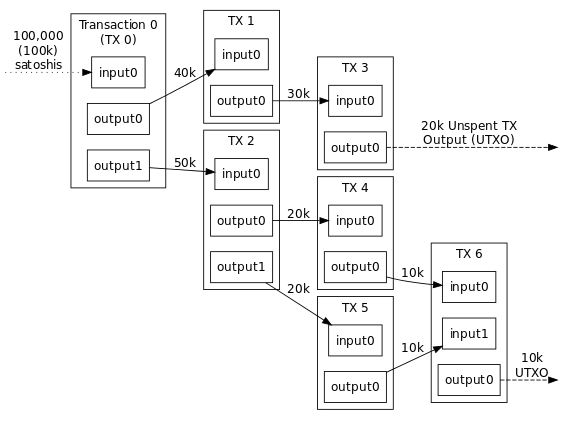
\includegraphics[height=8cm, width=10cm]{bitcoin_transactions_tree.png}
  \centering
  \caption{Árbol de transacciones (gráfico extraído de Bitcoin.org)}
  \label{fig:bitcoin-transactions-tree}
\end{figure}

En el árbol de transacciones precedente, puesto como ejemplo, coexisten solamente dos UTXO, la salida 0 de la transacción 3 y 6, por ser las únicas que aún no están siendo referenciadas por ninguna entrada de transacciones posteriores. Por el contrario, el resto de las salidas ya fueron relacionadas a otras entradas y, por ende, se consideran ``gastadas''. El problema del doble gasto se soluciona en principio de esta manera, es decir, evitando que una entrada se asocie a una salida previa ya referenciada. Y con respecto a calcular el balance de una dirección, basta sólo con consultar por todas las UTXO con dicha dirección y sumarizar el valor de cada una.

Ya presentada toda la terminología necesaria, ahora se presentará en mayor profundidad la estructura de las transacciones en Bitcoin, y fundamentalmente, el mecanismo de procesamiento y transferencia de los recursos. Se tomará como ejemplo la transacción 4 de la figura \ref{fig:bitcoin-transaction-bitcoincore} para mostrar cómo sería su composición en formato JSON y explicar en detalle las partes más importantes:

\begin{minipage}{\linewidth}
\begin{lstlisting}[frame=single, belowskip=1em, aboveskip=2em,  language=javascript, captionpos=b, caption=Estructura JSON de una transacción en Bitcoin, label={lst:estructura_transaccion}]
{
  "txid": "2cc6c24ad0d71f26...", // txid transaccion 4
  "version": 2,
  "size": ...,
  "vsize": ...,
  "locktime": 0,
  "vin": [
    {
      "txid": "1e71985325c3797b...", // txid transaccion 2
      "vout": 1,
      "scriptSig": {
        "asm": "001496d847228e50f6032a3837b3f7cc915e7291d240",
        "hex": "16001496d847228e50f6032a3837b3f7cc915e7291d240"
      },
      ...
    }
  ],
  "vout": [
    {
      "value": 6,
      "n": 0,
      "scriptPubKey": {
        "asm": "OP_DUP OP_HASH160 9545cfd22b756888fac4d2cca1dc6d389430acf2 OP_EQUALVERIFY OP_CHECKSIG",
        ...
      }
    },
    {
      "value": 2,
      "n": 1,
      "scriptPubKey": {
        "asm": "OP_DUP OP_HASH160 a2ca76b8716d612ae856d91d4b96c7c1a4f0a150 OP_EQUALVERIFY OP_CHECKSIG",
        ...
      }
    }
  ],
  // ...(metadatos del bloque correspondiente)...
  "time": 1551289194,
},
\end{lstlisting}
\end{minipage}

Del extracto JSON del ejemplo anterior, y en general para cualquier transacción de Bitcoin, se pueden identificar tres grandes grupos:

\begin{itemize}
  \item \textbf{Metadatos}: entre los metadatos figuran el identificador de la transacción (\textit{txid}), versión de la especificación (\textit{version}), tamaño de la transacción (\textit{size} y \textit{vsize}), momento de la transacción (\textit{time}) y datos referidos al bloque que contiene a la transacción.
  \item \textbf{Lista de entradas}: representado por medio de un \textit{array} bajo la clave \textit{vin}. Por cada entrada se registra la transacción y el índice de la salida UTXO a reclamar (\textit{txid} y \textit{vout}, respectivamente) y un código de desbloqueo (\textit{scriptSig}) que será requerido para poder autenticar esta acción de forma correcta.
  \item \textbf{Lista de salidas}: representado también por medio de un \textit{array} bajo la clave \textit{vout}. Cada salida tiene información de su valor monetario (\textit{value}), su índice (\textit{n}) y un código de bloqueo (\textit{scriptPubKey}) con información relacionada al beneficiario que sólo él podrá desbloquear al momento de hacer el reclamo de estas salidas (que así como están son UTXO dado que no han sido gastadas o reclamadas aún).
\end{itemize}

La mayoría de los datos presentes en una transacción de Bitcoin ya han sido desarrollados previamente. Resta comprender cómo se validan y autorizan las mismas, cuya clave se encuentra en los códigos de bloqueo y desbloqueo. Más precisamente, estos son sentencias de un lenguaje ensamblador (de ahí surgen las claves \textit{asm} del listado \ref{lst:estructura_transaccion}) propio de la plataforma. Esto es así dado que la red Bitcoin posee varios tipos de transacciones de acuerdo a qué partes de la transacción se incluyen para la firma, y por diseño, se delegan las reglas y las validaciones de estos distintos tipos en este microlenguaje\footnote{Está específicamente diseñado para validación de transacciones monetarias y, por tal razón, y para evitar problemas de seguridad computacional, no es Turing-completo.} que otorga suficiente flexibilidad para soportar los diferentes esquemas de comprobación existentes, e incluso, agregar otros\footnote{En la práctica, sin embargo, se ha limitado la inclusión libre de otros esquemas por razones de seguridad.} sin comprometer el diseño nuclear de Bitcoin.

A continuación, se explicará el caso más común y simple, es decir, el de un emisor generando una o muchas salidas, el cual se encargará de firmar toda la transacción. Hacer una transferencia implicará que el emisor reclame un número suficientes de salidas no gastadas para cubrir los fondos a transferir, y con ellos, construir las entradas de la nueva transacción. Pero tales entradas requerirán, a su vez, códigos de desbloqueo para liberar los activos de esas salidas y demostrar, ante toda la red, que el emisor es el dueño autorizado para tal fin. Para ello, el emisor deberá armar previamente la transacción con las salidas y los activos listos a transferir al siguiente beneficiario junto a las salidas UTXO que intentará reclamar el emisor. Esto último será temporal, dado que en realidad deberían ir las entradas para que la transacción sea válida; en breve se entenderá el porqué. Tras esto, se obtiene una huella digital de la construcción previa y se firma la huella con una clave privada del emisor. Este paso es el que corresponde a la autorización de toda la transacción por parte del emisor (ver figura \ref{fig:bitcoin-transaction-paper}). Finalmente, a la firma obtenida se le concatena la clave pública del emisor. Estos dos datos conforman el código de desbloqueo que, ahora sí, se usan para armar las entradas faltantes y sustituirlas por las salidas temporales que se colocaron previamente. Antes, no era posible armar las entradas de arranque porque justamente se necesitaba para ello la firma total de la transacción con, al menos, las salidas referenciadas.

Ahora bien, resta explicar cómo funciona el mecanismo de bloqueo y desbloqueo en las transacciones. Como se ha establecido anteriormente, se utiliza un microlenguaje para ejecutar la validación de las mismas, que se encuentra embebido allí mismo por razones de versatilidad. Para determinar si una transacción, o más específicamente, si las entradas de la misma se encuentran autorizadas a hacer uso o gasto de las salidas referenciadas, lo que se hace -desde el punto de vista de un tercero, por ejemplo- es copiar el código de desbloqueo de la/s entrada/s (\textit{scriptSig}) y, a continuación, el código de bloqueo de la salida UTXO referenciada (\textit{scriptPubKey}). Únicamente se autorizará y validará correctamente la transacción si y sólo si la ejecución de esa secuencia de códigos resulta exitosa, es decir, sin ninguna falla o problema.

Una validación de propiedad de una transacción simple es como sigue:

\begin{figure}[H]
  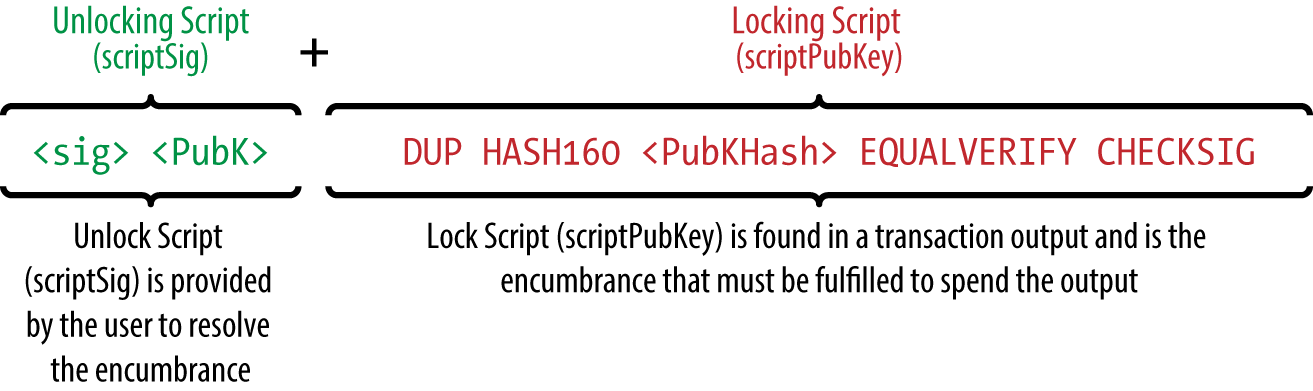
\includegraphics[height=5cm, width=14cm]{bitcoin_transaction_validation.png}
  \centering
  \caption{Validación de propiedad de una transacción evaluando los códigos de desbloqueo y bloqueo}
  \label{fig:bitcoin-transaction-validation}
\end{figure}

La ejecución procede de izquierda a derecha, ejecutando instrucción por instrucción. Una característica importante a destacar del lenguaje de \textit{scripting} de Bitcoin es que es orientado a pila, con lo cual, las instrucciones operarán siempre con datos en una estructura de tipo LIFO (\textit{Last-In-First-Out}, ``el último dato que ingresa es el primero en salir''). Otra propiedad del lenguaje es que, por un lado, se tienen instrucciones que procesan datos de la pila y, por otro lado, se tienen simplemente datos que al aparecer en la línea de ejecución se apilan en la estructura de datos global del entorno.

Explicado el modelo de ejecución básico del lenguaje de Bitcoin, se procederá a examinar la ejecución de validación de la figura \ref{fig:bitcoin-transaction-validation}. En la figura \ref{fig:bitcoin-stacktrace-example} se mostrarán los cambios en la pila para ayudar a seguir la ejecución:

\begin{enumerate}
  \item Al principio de la línea de ejecución figuran los dos principales componentes del código de desbloqueo provenientes de una entrada de la transacción a validar: la firma (\textit{sig}) y la clave pública (\textit{PubK}) asociada a la clave privada de dicha firma. Dado que son simplemente datos, primero se apila la firma, y luego la clave pública, siendo este último dato ahora el tope de la pila.
  \item Luego arranca la ejecución del código de bloqueo que hará la verificación real. En primer lugar, se ejecuta la instrucción \textit{DUP} cuya función es copiar el dato en el tope de la pila y volver a apilarlo.
  \item Luego se ejecuta la instrucción \textit{HASH160} que lo que hace básicamente es obtener un \textit{hash} del último dato en la pila, el cual además, es quitado de la pila; en concreto, se termina ejecutando \textit{HASH160 PubK}. Finalmente este resultado es apilado.
  \item Se apila \textit{PubKHash} que representaría la dirección destino de los fondos, o lo que coloquialmente se conoce dentro de la red Bitcoin como dirección Bitcoin\footnote{Es algo coloquial dado que conceptualmente hay que recordar que no existe la idea de dirección o cuenta en Bitcoin, es tan sólo una construcción por encima de la red.}.
  \item La instrucción \textit{EQUALVERIFY} simplemente remueve los dos últimos datos de la pila y comprueba si son iguales. Esto significa que lo que se hace es comparar la dirección destino previamente apilada contra el valor \textit{Hash-160} de la clave pública provista de antemano en el código de desbloqueo, el cual debería producir la mencionada dirección. En otras palabras, esta verificación tiene como fin comprobar que la dirección o clave pública del reclamante de las salidas UTXO es el mismo que figura en dichas salidas. En caso de no ser iguales, la ejecución y la validación fallará y la transacción será declarada inválida.
  \item Por último se ejecuta la instrucción \textit{CHECKSIG}. Su complejo trabajo consiste en constatar que la firma de la transacción es válida en función de la clave pública, ambos datos provistos desde el código de desbloqueo. Con esto, lo que se valida es que el reclamante de los fondos de las salidas no gastadas es verdaderamente el destinatario autorizado a gastarlas, ya que únicamente él con su clave privada pudo haber construido dicha firma, ratificada con la clave pública entregada.
\end{enumerate}

\begin{figure}[H]
  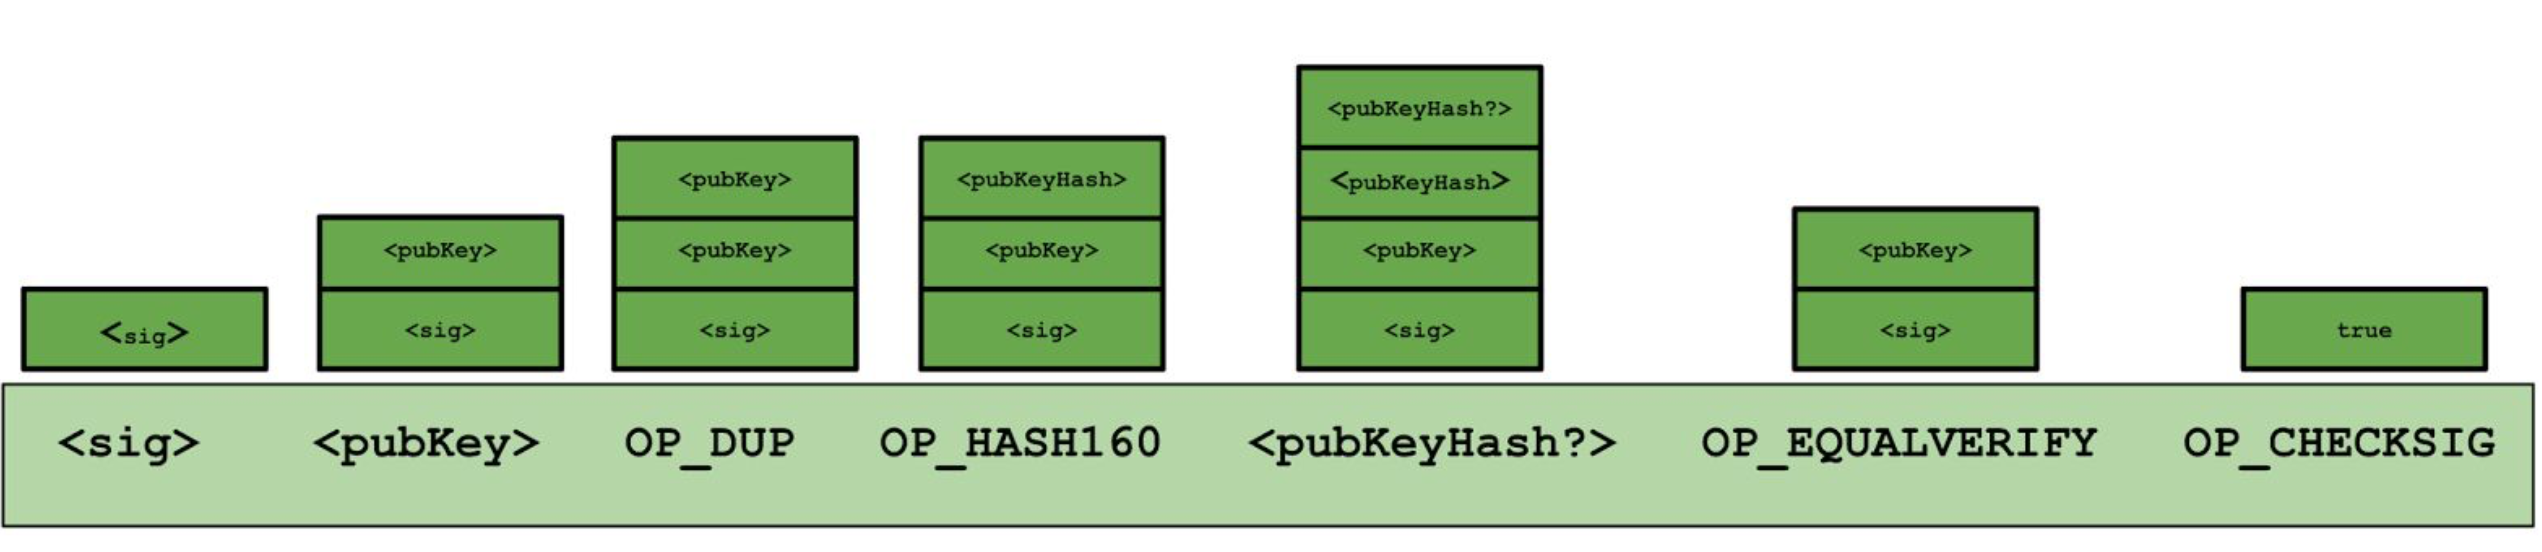
\includegraphics[height=3cm, width=14cm]{bitcoin_stacktrace_example.png}
  \centering
  \caption{Seguimiento de los cambios en la pila durante la ejecución de la validación}
  \label{fig:bitcoin-stacktrace-example}
\end{figure}

Tal como se mencionó, si toda la línea de ejecución termina sin errores, entonces la validación de propiedad resultará exitosa y las salidas reclamadas pasarán a estar en estado ``gastadas''.

\paragraph{Bloque}
\label{bc_bitcoin_block}

Un bloque es una estructura que agrupa transacciones, básicamente. Si bien, desde un punto de vista puramente teórico, la blockchain de Bitcoin podría funcionar sin el concepto de bloque, la realidad es que es un fundamento imprescindible en la práctica a la hora de validar y sincronizar transacciones eficientemente, siendo muy significativa la diferencia en rendimiento entre hacer estas tareas en lote que si se hicieran individualmente por transacción.

En primer lugar, y similar a como sucede con las transacciones, los bloques también se encadenan unos con otros, formando una cadena de bloques -o \textit{blockchain}-:

\begin{figure}[H]
  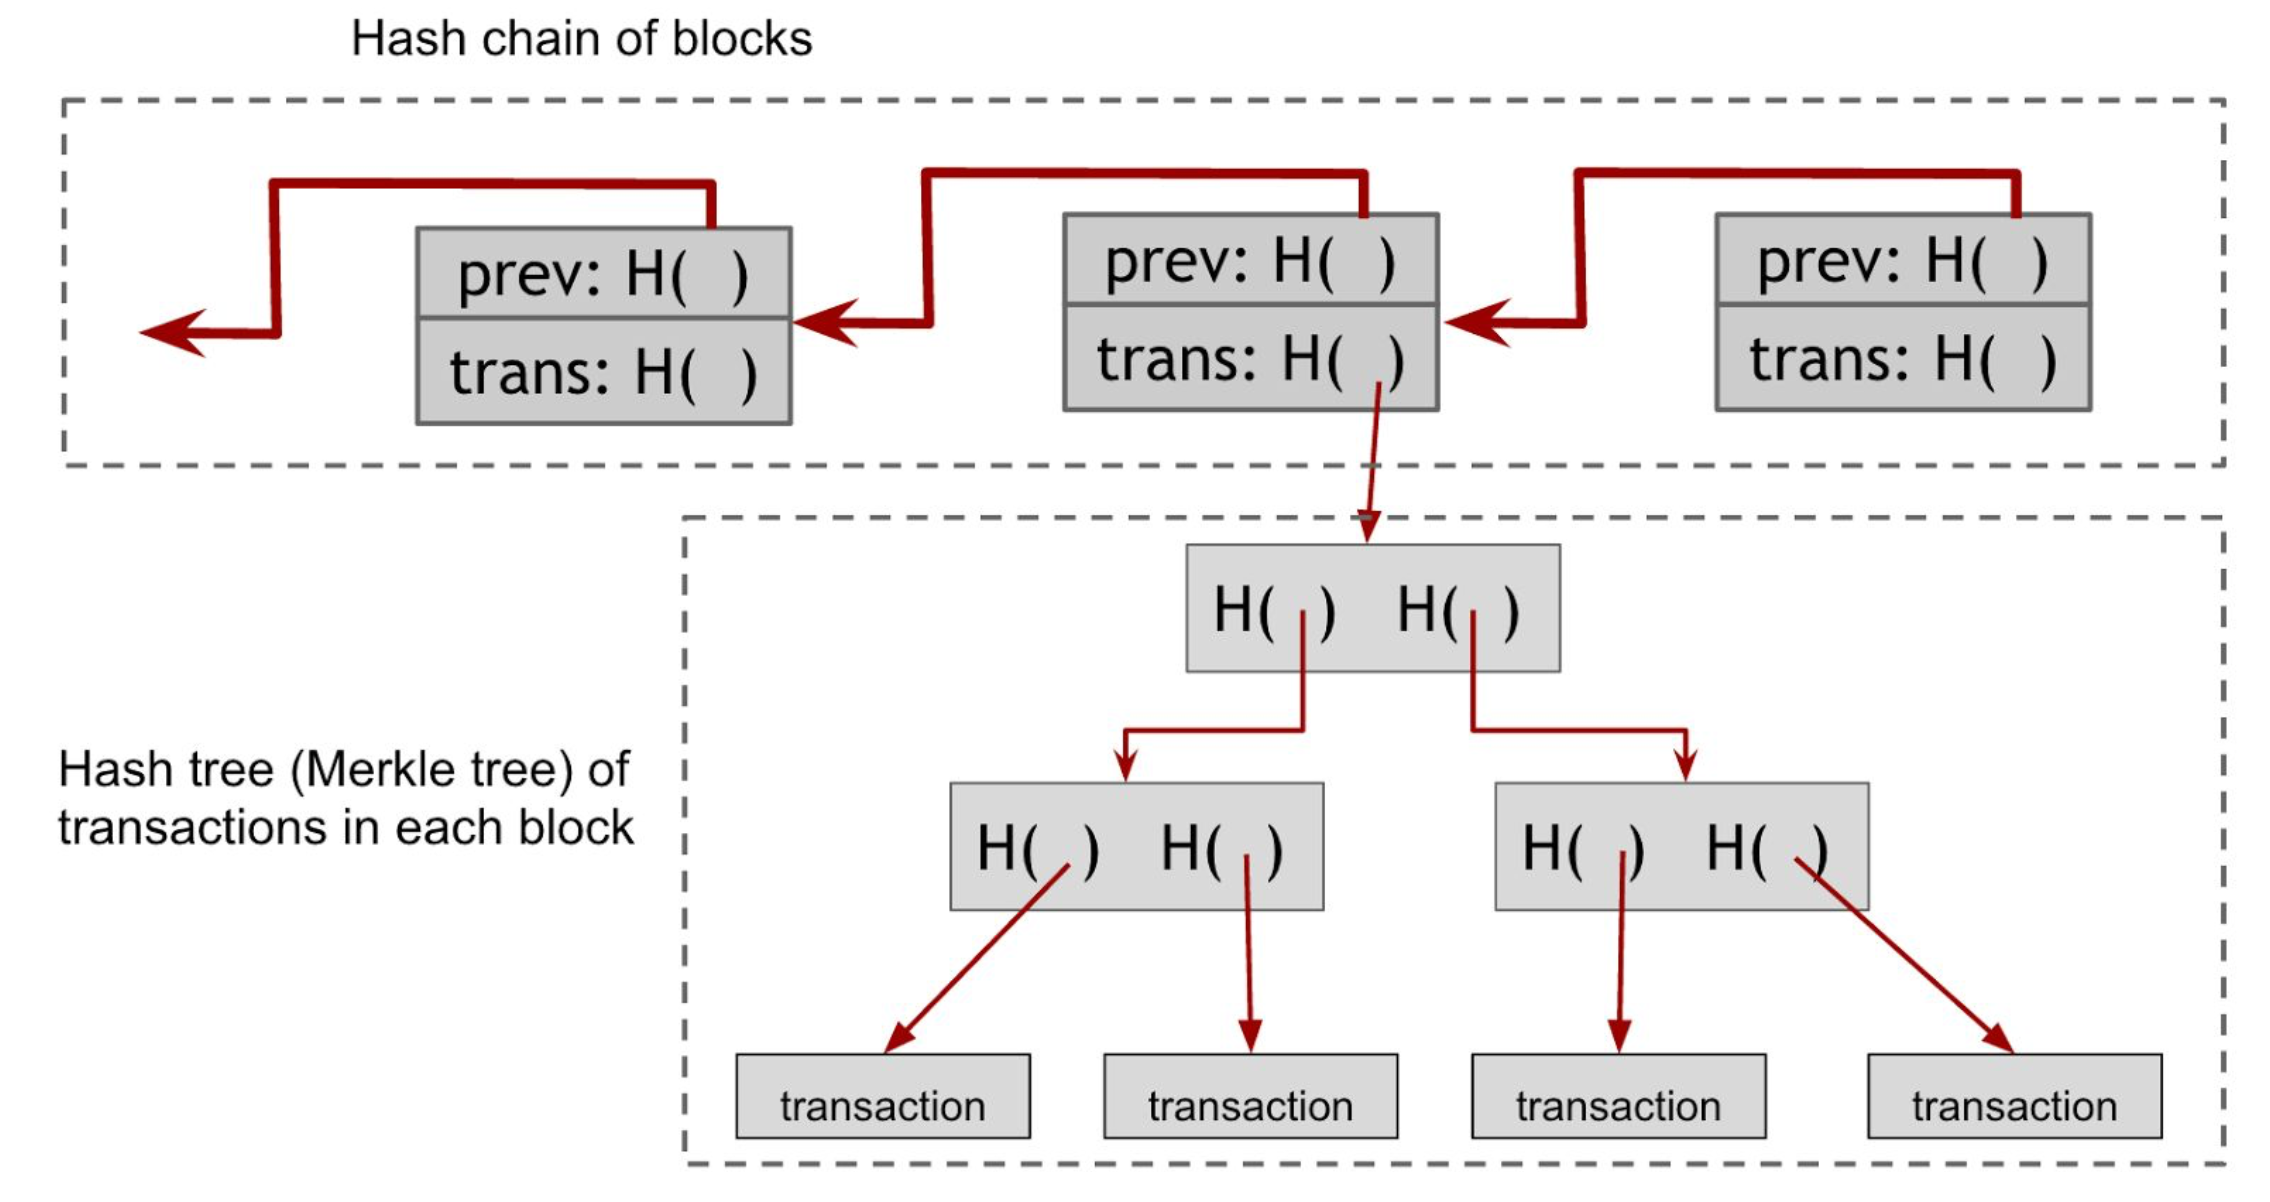
\includegraphics[height=8cm, width=14cm]{bitcoin_blockchain.png}
  \centering
  \caption{Cadena de bloques en Bitcoin}
  \label{fig:bitcoin-blockchain}
\end{figure}

Como se puede ver, la figura \ref{fig:bitcoin-blockchain} remite mucho a lo ilustrado en las secciones \ref{bc_origins_blockchain} y \ref{bc_origins_merkle}, donde se define la idea de cadena de bloques y luego la inclusión de árboles de Merkle en ellas. Pues bien, aquí los conceptos serán esencialmente los mismos, es decir, se usará una cadena de bloques para proteger la integridad de los datos -en este caso, serían las transacciones- a medida que la misma crece, ya que cada bloque contendrá una huella digital de su cabecera, donde allí, habrá una referencia de la huella digital del bloque anterior. Y tal como se explicó en \ref{bc_origins_blockchain}, si un dato es alterado en un bloque previo, entonces dicho cambio repercutirá en los bloques siguientes puesto que el valor computado de sus huellas depende parcialmente de esas referencias hacia atrás en los bloques.

Por otra parte, también como se puede ver en la figura \ref{fig:bitcoin-blockchain}, cada cabecera de bloque guarda una huella digital especial conocida como \textit{raíz Merkle} la cual sirve para validar eficientemente la integridad y la pertenencia de las transacciones que forman parte de un bloque determinado. Tal como se ha indicado en el apartado \ref{bc_origins_merkle}, el uso de árboles Merkle permite validar eficientemente -en orden de tiempo y espacio logarítmico- si una transacción se encuentra incluida en un bloque, además de proteger la integridad del bloque en caso que se agreguen, quiten o se alteren transacciones dentro de dicho bloque. Estas propiedades permiten que existan nodos que validen la veracidad de una transacción sin requerir toda la información o todas las transacciones del bloque.

A continuación se mostrará la estructura de un bloque de ejemplo en formato JSON:

\begin{minipage}{\linewidth}
\begin{lstlisting}[frame=single, belowskip=1em, aboveskip=2em,  language=javascript, captionpos=b, caption=Estructura JSON de un bloque en Bitcoin, label={lst:estructura_bloque}]
{
  // Cabecera del bloque
	"version": 536870912,
	"versionHex": "20000000",
  "hash": "0000000000000000001a293907c5e1da...",
	"chainwork": "00000000000000000000000000000000...",
	"previousblockhash": "00000000000000000011b49510c6413d...",
	"nextblockhash": "0000000000000000000a2a15026aab26...",
	"merkleroot": "eeae080affb6c38462aec166c6abcd96...",
	"confirmations": 20,
	"strippedsize": 874261,
	"size": 1370613,
	"weight": 3993396,
	"height": 565664,
  "time": 1551727185,
	"mediantime": 1551725107,
	"nonce": 3827230916,
	"bits": "172e5b50",
	"difficulty": 6071846049920.752,
  // Array de todas las transacciones
  "tx": [
    // ...
  ]
}
\end{lstlisting}
\end{minipage}

Por un lado se tienen los datos de la cabecera, que podrían dividirse lógicamente en los siguientes grupos:

\begin{itemize}
  \item Huella del bloque: el campo \textit{hash} es la huella digital del bloque. Presenta características especiales referentes al minado y al consenso, que serán explicadas posteriormente.
  \item Referencias a otros bloques: los campos \textit{previousblockhash} y \textit{nextblockhash} contienen las huellas digitales del bloque antecesor y posterior, respectivamente
  \item Campos referentes al minado: \textit{nonce}, \textit{time} y \textit{difficulty} son campos relacionados al proceso de minado del bloque que se explicará luego.
  \item \textit{merkleroot}: referencia o huella de la raíz Merkle.
  \item Tamaño y altura: \textit{size} representa el tamaño total del bloque incluyendo las transacciones y \textit{height} denota la altura, esto es, el índice de bloque que le corresponde contando desde el primer bloque de la cadena, o bien, bloque génesis.
\end{itemize}

Y al final, se incluye el conjunto de todas las transacciones que pertenecen al bloque.

\subsubsection{Consenso y minado}

Esta sección versará sobre el consenso distribuido entre todos los participantes de la red, es decir, cómo alcanzan un acuerdo común sobre qué transacciones son válidas o no y el minado que es la forma de implementar dicha tarea.

Dado que Bitcoin y su blockchain conforman una red distribuida, no existe una entidad o grupo de confianza al cual delegarle la verificación de las transacciones que se realizan sobre esta arquitectura. En términos equivalentes, no se dispone de un estado global administrado por un único veedor (por ejemplo, una base de datos en un sistema centralizado). En su lugar, se requieren estrategias para alcanzar un acuerdo unánime, o al menos mayoritario, sobre dicho estado de manera distribuida y ecuánime. Esto, en la terminología de sistemas distribuidos, es lo que se conoce como consenso distribuido.

\paragraph{Problema de los Generales Bizantinos}
\label{bc_bitcoin_gbp}

Para comenzar con el análisis del consenso en Bitcoin, hay que tener en cuenta que la red -como ya se ha establecido- se encuentra distribuida geográficamente por todo el planeta y los usuarios finales son personas. La razón por la cual se exponen estás dos propiedades es para dejar asentado que en el funcionamiento regular de este sistema, la desconfianza será una variable siempre presente, ya sea fortuita, como en el caso de problemas técnicos en los enlaces o en los nodos conformantes de dicha red, o bien, intencional, como en el caso de que existan participantes deshonestos intentando conseguir alguna ventaja a través de técnicas espurias.

Un interesante trabajo al respecto publicado en 1982 por los científicos Leslie Lamport, Robert Shostak y Marshall Pease, titulado ``El Problema de los Generales Bizantinos''\cite{Lamport82thebyzantine} emplea como analogía un escenario de guerra en el cual una ciudad enemiga se encuentra sitiada por varias divisiones lideradas cada una por un general bizantino. Todos ellos deben consensuar una orden en donde las posibilidades son ``atacar'' o ``retirarse''. Y el problema es que algunos de esos generales pueden ser traidores, esto es, comunicar órdenes contradictorias al momento del consenso de manera tal de confundir al resto de los generales. Asimismo, en el marco de este problema, quien inicia la orden es denominado ``Comandante'' y el resto de los generales ``Tenientes''. Establecido esto, una solución a este problema con $n$ generales es aquella en la cual, dado un Comandante que envía la orden a sus $n - 1$ Tenientes, se garantizan las siguientes condiciones:

\begin{enumerate}
  \item Todos los Tenientes leales obedecen la orden impartida por el Comandante.
  \item Si el Comandante es leal, entonces cada Teniente leal obedecerá la orden que el Comandante impartió.\footnote{La 2da condición es más fuerte que la 1era}
\end{enumerate}

Es importante remarcar que estas condiciones son las que cualquier algoritmo de consenso debería tratar para resolver el problema de los generales bizantinos. Además, cualquier sistema que resuelva o sea inmune a este tipo de fallas se lo denomina tolerante a fallas bizantinas.

En el trabajo de Lamport se analizan diferentes casos según la cantidad de generales y traidores y según el canal de comunicación -oral o escrito-. En el más general de todos los casos, con $m$ generales, se requiere que más de dos tercios de esos $m$ generales sean honestos y/o leales.

Asimismo, se plantean algunas soluciones teóricas al problema, pero recién en el año 1999, Miguel Castro y Barbara Liskov publicarían una variante de solución junto a una implementación probada tanto en correctitud como en rendimiento\cite{Castro:1999:PBF:296806.296824}, pero presenta dos problemas: en primer lugar, nunca fue bien probado en arquitecturas grandes y se sospecha que no escala muy bien dada la gran cantidad de mensajes que deben intercambiarse para lograr un consenso mayoritario. Y por último, y quizás más importante, es que el funcionamiento del mismo depende de la autenticación de los nodos, lo cual, en blockchains públicas y anónimas como Bitcoin es inadmisible. Por estas razones, normalmente las blockchains que utilizan este algoritmo de consenso en la actualidad son pequeñas y privadas, donde incluso, hay nodos que están bien identificados ante todos.\footnote{\href{https://blockonomi.com/zilliqa-guide/}{Zilliqa}, \href{https://www.hyperledger.org/projects/fabric}{Hyperledger}, \href{https://neo.org/}{Neo}}

\paragraph{Prueba de trabajo}
\label{bc_bitcoin_pow}

Satoshi Nakamoto propuso en su diseño de la blockchain de Bitcoin usar Prueba-de-Trabajo (o PoW, del inglés Proof-of-Work) como algoritmo de consenso. La razón fundamental para sustentar su decisión es que permite consenso entre pares sin requerir autenticación o prueba de identidad. El único requisito, suficiente para colocar un nuevo bloque dentro de la cadena, es demostrar que se ha realizado un trabajo computacional exhaustivo para ello. Claramente esto está fuertemente inspirado en lo realizado por Adam Back en Hashcash, explicado previamente en la sección \ref{bc_origins_hashcash}.

Cuando no se puede contar con identidades en un sistema distribuido y es necesario validar o lograr un consenso de algún tipo, uno de los potenciales problemas de seguridad a atacar es impedir que nodos maliciosos difundan información ilegítima en la red y consigan que ella sea parte de su estado global. Esto es lo que se conoce como ataque \textit{Sybil}.

La prueba de trabajo evita este tipo de ataques forzando a que el costo de validar un bloque para tener la chance de ser incluida en la cadena de bloques sea muy alto, con lo cual, ya no tendría más sentido la ventaja de controlar gran cantidad de nodos para intentar adulterar la red, salvo que se disponga de mucho poder computacional, lo cual será analizado en la sección \ref{bc_bitcoin_security}.

La siguiente cuestión a resolver es cómo compensar a aquellos participantes honestos de la red que invierten su poder computacional para mantener el buen funcionamiento de la red. Y es tal vez aquí donde entra en escena una de las principales innovaciones de Bitcoin respecto a los algoritmos de consenso, y es el incentivo a través del minado. Bitcoin es una cadena de bloques de transacciones monetarias, con lo cual, posee como propiedad que las transacciones tienen un valor económico. En general, en la gran mayoría de las transacciones intervienen dos participantes o grupos, quien transfiere fondos y el/los beneficiarios. No obstante, existe un tipo de transacción especial denominada ``\textit{Coinbase transaction}'' (se podría traducir aproximadamente a ``transacción de acuñado o minado'') que todo bloque debe poseer para ser considerado válido. Este tipo de transacción crea o emite monedas, es decir, no tiene entradas, sólo una o más salidas hacia direcciones arbitrarias, normalmente, direcciones propias del participante que está realizando la validación de ese bloque. De esta forma, si el bloque es aceptado por el consenso distribuido, el nodo que realizó la validación y la prueba de trabajo pertinente tendrá como recompensa el derecho de gastar la entrada que generó monedas. Por esta razón, esto también se conoce como minado, puesto que se realiza un trabajo muy arduo en pos de obtener a cambio una retribución monetaria.

La prueba de trabajo en sí, en Bitcoin, consiste en hallar un número \textit{nonce} (mencionado en \ref{bc_bitcoin_block}) tal que la huella digital computada de él junto a la información de la cabecera del bloque, como por ejemplo, el \textit{hash} puntero al bloque previo y los \textit{hashes} que resumen a todas las transacciones contenidas (el \textit{merkleroot}) den un número de \textit{hash} menor a un objetivo -\textit{target}-, o de forma equivalente, den un \textit{hash} que comience con determinada cantidad de ceros. Formalmente sería:

\begin{equation}
H(nonce \| hash\_previo \| merkleroot) < target
\end{equation}

Dada la aleatoriedad de la función de hash $H$, encontrar el $nonce$ que satisfaga la inecuación es una tarea de fuerza bruta, y por consiguiente, muy ardua. Quien consiga resolver la prueba, por otra parte, tiene derecho a difundir su bloque de transacciones con su prueba de trabajo y el resto de los participantes podrá realizar las verificaciones pertinentes, incluso la de la prueba de trabajo, de una forma muy sencilla. Otro de los parámetros mencionados en \ref{bc_bitcoin_block} era la dificultad -\textit{difficulty}-, el cual es un factor que permite reajustar el \textit{target} de manera tal que la prueba de trabajo sea más fácil o más difícil de resolver. Este parámetro es controlado dinámicamente por toda la red en pos de mantener un tiempo promedio de validación de bloques de 10 minutos. La razón de esta cifra es algo arbitraria, pero en la práctica de la red Bitcoin funciona razonablemente bien. Con menos tiempo se corre el riesgo de sobrecargar la red con nuevos bloques -perdiendo rendimiento- y con más tiempo haría que la confirmación de las transacciones sea demasiado lenta.

Queda pendiente ver cómo es la confirmación de los bloques y si realmente este método es tolerante a fallas bizantinas. Pero para ello será necesario avanzar un poco en explicar la mecánica general de la red Bitcoin.

\subsubsection{Funcionamiento de la red}
\label{bc_bitcoin_net_overview}

En esta sección se describirá y analizará el funcionamiento global de la red Bitcoin. Lo primero a tener en cuenta es que en la red Bitcoin, al ser una red P2P\footnote{\textit{Peer-to-Peer} ``Par a par''}, todos los nodos tienen la capacidad de realizar las mismas tareas, es decir, poseen el mismo potencial para realizar cualquier trabajo que sea requerido por la red. De todas formas, en la realidad, cada nodo normalmente posee un rol dentro de la red, pero no existe restricciones explícitas sobre tales asignaciones. Dicho esto, a continuación se citarán los pasos de ejecución de la red, descritos en el \textit{paper} de Nakamoto:

\begin{enumerate}
  \item Las transacciones nuevas se transmiten a todos los nodos.
  \item Cada nodo recoge todas las transacciones en un bloque.
  \item Cada nodo trabaja en resolver una prueba de trabajo compleja para su bloque.
  \item Cuando un nodo resuelve una prueba de trabajo, transmite el bloque a todos los nodos.
  \item Los nodos aceptan el bloque si todas las transacciones en él son válidas y no se han gastado con anterioridad.
  \item Los nodos expresan su aceptación del bloque al trabajar en crear el siguiente bloque en la cadena, usando el \textit{hash} del bloque aceptado como \textit{hash} previo.
\end{enumerate}

Cuando un nodo crea una transacción, ésta se propaga a través de los nodos vecinos y así sucesivamente hasta cubrir toda la red. Cada nodo es capaz por sí mismo de validar las transacciones de forma independiente, dada la naturaleza P2P de la red. Un nodo difunde la transacción sobre el resto si y sólo si la misma es válida, de lo contrario, es descartada. Una vez validadas por el nodo, las transacciones se recopilan temporalmente en una memoria denominada \textit{mempool}: allí residen todas las transacciones que han sido recibidas y validadas por un nodo particular. Luego, un nodo selecciona y remueve de esa \textit{mempool} unas cuantas transacciones para conformar un bloque y trabaja en resolver la prueba de trabajo para él. Durante este proceso, puede suceder que el nodo reciba otros bloques válidos en donde las transacciones coincidan con las que están en vías de validación, en cuyo caso, el nodo deberá reiniciar el trabajo con un nuevo bloque y otras transacciones no confirmadas en la cadena aún, eliminando las transacciones ya validadas por otros nodos de su propia \textit{mempool}. Si, en cambio, el nodo consigue resolver la prueba de trabajo de su bloque, éste se transmite al resto de los nodos los cuales realizarán las validaciones pertinentes, es decir, revisarán que todas las transacciones conformantes sean legítimas y corroborarán la prueba de trabajo. Si es válida, cada nodo comienza a trabajar sobre un nuevo bloque partiendo del aceptado -el \textit{hash} previo del nuevo bloque será el \textit{hash} de este último bloque- y propaga el recibido sobre los otros nodos, mientras que si no es válido -ya sea por alguna transacción defectuosa o espuria, o porque la prueba de trabajo no es legítima-, lo rechaza y no lo transmite al resto de la red (tal como sucede con una transacción individual).

Lógicamente, dado el funcionamiento concurrente y descentralizado de la red, puede darse casos en dónde más de un nodo difundan bloques válidos hacia el resto en una ventana relativamente corta de tiempo, de manera tal que la cadena de bloques diverge temporalmente, esto es, hay varios bloques apuntando a un mismo bloque previo a la vez. Este problema se resuelve eventualmente teniendo presente que siempre, en todos los casos, los nodos eligen extender la cadena de bloques más larga en caso de existir divergencias. Por supuesto, tal como se mencionó recién, pueden generarse situaciones en donde existan en momentos puntuales dos cadenas de igual longitud que sean válidas, pero a lo largo del tiempo, dada la competencia entre los nodos por validar bloques rápidamente, estos mismos decidirán extender una de esas cadenas y las otras serán descartadas automáticamente, prevaleciendo en el tiempo siempre una única cadena. Analizándolo desde otra perspectiva, es improbable que dada una bifurcación, ésta perdure en el tiempo a través de dos cadenas de longitud equivalente, a menos que la mitad de los nodos de la red coordinen para apoyar el crecimiento de una, mientras que la otra mitad mantiene la otra cadena, respectivamente.

Elegir extender determinada cadena de bloques, como decisión, representa dar un voto con el poder de cómputo del nodo. Dado que la regla de facto en la red es siempre extender la cadena más larga, está cadena será, en consecuencia, aquella con la mayor cantidad de trabajo acumulado. Y esto mismo es lo que permite, en el tiempo, lograr el consenso distribuido requerido. En referencia al Problema de los Generales Bizantinos desarrollado en \ref{bc_bitcoin_gbp}, se puede establecer un paralelismo entre las condiciones o propiedades necesarias para una posible solución y algunas de las características del consenso en Bitcoin:

\begin{enumerate}
  \item Todos los nodos honestos trabajan en la colocación de los bloques dentro de la cadena principal.
  \item Si un bloque es válido, entonces cada nodo honesto trabajará en colocar ese bloque en la cadena principal.
\end{enumerate}

Esto, en concordancia con el incentivo a cada nodo validador y la prueba de trabajo, hace que la red en la práctica sea tolerante a fallas bizantinas dado que, por un lado, las fallas aleatorias o triviales, como por ejemplo, defectos en los bloques o en las transacciones, son descartados por cada nodo y, por otro lado, las fallas deshonestas son muy difíles de llevar a cabo bajo este sistema, tal cómo se analizará en la próxima sección.

\subsubsection{Robustez y/o seguridad de la red}
\label{bc_bitcoin_security}

En esta sección se cubrirán algunos de los principales y posibles ataques que podría sufrir la red blockchain y cómo la misma garantiza un nivel de seguridad lo suficientemente aceptable como para realizar transacciones monetarias.

En primer lugar, se podría plantear la duda más primordial y también severa acerca de si las ``monedas'' podrían robarse de algún modo. A menos que se encuentren fallas en los algoritmos de criptografía asimétrica utilizados, realizar esto es imposible. Recordar de la parte \ref{bc_bitcoin_transaction} que dichas ``monedas'' se representan como salidas no gastadas (UTXO) y la única manera de reclamarlas es utilizando la clave privada -la cual es única para el beneficiario de esas salidas- adecuada dentro del código de desbloqueo de las entradas generadas en la nueva transacción, de manera tal de liberar el código de bloqueo de la salidas y así hacer que la transacción sea válida.

Otro posible ataque menor es la denegación de servicio, esto es, hacer que deliberadamente determinadas transacciones no conformen bloques con la idea de que no se integren nunca a la cadena, teniendo presente que cada nodo es libre de elegir las transacciones que usará para validar un bloque. El hecho de que uno o más nodos coordinen para no elegir ciertas transacciones no basta para que éstas no sean incluidas en la cadena eventualmente, ya que el resto de los nodos independientes trabajarán para incluir a todas las transacciones presentes en la red, sin distinción. Mientras el grupo honesto e independiente de nodos sea mayor al maligno, este ataque no podrá tener éxito.

Luego, existe otro tipo de ataque muy estudiado -que incluso aparece en el paper de Nakamoto- que es el ``ataque del doble gasto''. Esto consiste en crear dos transacciones (cada una con una entrada) que reclamen una misma salida UTXO. El doble gasto dentro de una única cadena está prohibido ya que, como se ha visto, la transacción será válida si las salidas a consumir no han sido referenciadas en otras transacciones, es decir, no fueron gastadas. Pero podría darse está situación en dos cadenas: una primera transacción $t_1$ que consuma una salida $s$ dentro de un bloque de la cadena actual y una segunda transacción $t_2$ que consuma la misma salida $s$ pero en un bloque de la cadena alternativa. Dado que $t_1$ y $t_2$ hacen referencia a la misma salida $s$, sólo una de ellas podrá ser incluida en la cadena principal (la otra será invalidada y, por ende, descartada). Si esas cadenas tienen la misma longitud, cualquiera de esas dos transacciones podrán ser aceptadas con igual probabilidad, ya que no hay preferencias acerca de qué cadena seguir extendiendo. En este tipo de ataques, en general, $t_1$ es una transacción honesta desde un usuario $A$ hacia un usuario $B$, en donde $A$ espera, a cambio de la transacción, algún valor proveniente de $B$ -un producto o un servicio- y luego de este evento, $A$ genera la transacción $t_2$ malintencionada -aunque no inválida por el momento- destinada a una dirección $A'$ -controlada por $A$- diseñada para seguir manteniendo los fondos de $A$ intactos y, asimismo, invalidar la transacción $t_1$ que hizo el gasto real. Si el ataque es exitoso, $A$ se habrá quedado con el valor de $B$ sin haber realizado gasto alguno.

Un ejemplo muy similar a lo expuesto previamente se grafica a continuación:

\begin{figure}[H]
  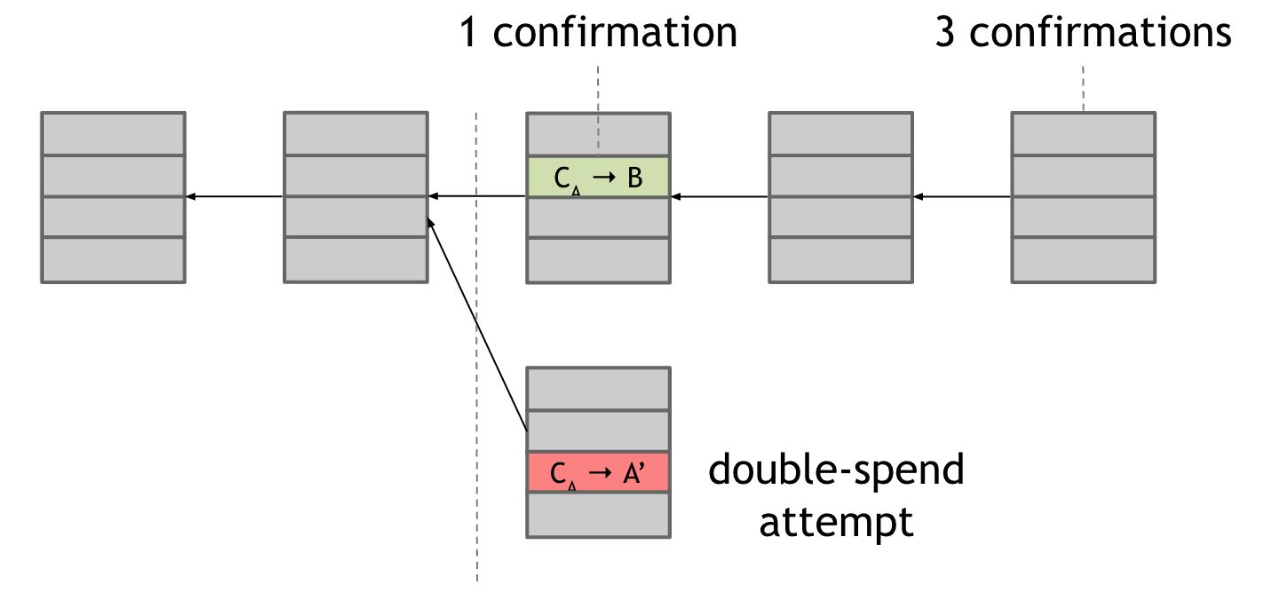
\includegraphics[height=6cm, width=12cm]{bitcoin_double_spend_example.png}
  \centering
  \caption{Ejemplo de ataque de doble gasto}
  \label{fig:bitcoin-double-spend-example}
\end{figure}

En donde $C_A \rightarrow B$ sería la transacción $t_1$ y $C_A \rightarrow A'$ representaría a la transacción $t_2$.

Dado que un ataque de doble gasto es una de las formas más sencillas de crear una historia alternativa de la cadena principal, la misma se emplea como caso de estudio maestro a la hora de analizar la robustez de la red. En el análisis probabilístico que realizó Satoshi Nakamoto -y otros autores como se ve en \cite{DBLP:journals/corr/OzisikL17} y en \cite{DBLP:journals/corr/Rosenfeld14}-, básicamente los parámetros que se encuentran siempre presentes en dichos estudios son:

\begin{enumerate}
  \item La probabilidad de que algún nodo honesto encuentre el siguiente bloque, la cual, es directamente proporcional al poder de cómputo controlado por dicho grupo de nodos.
  \item La probabilidad de que algún nodo deshonesto encuentre el siguiente bloque, la cual, es directamente proporcional al poder de cómputo controlado por dicho grupo de nodos.
  \item La cantidad de confirmaciones que presenta la cadena honesta respecto al bloque a atacar. Dicho de otra manera, la cantidad de bloques a reescribir y validar hasta llegar a alcanzar la longitud de la cadena principal (honesta).
\end{enumerate}

En el estudio de Nakamoto se formula el problema en términos de la siguiente ecuación:

\begin{equation}
  q_z = \begin{cases*}
    1         & \text{si} $p \leq q$\\
    (q/p)^z   & \text{si} $p > q$
        \end{cases*}
\end{equation}

donde $p$ y $q$ corresponden a los puntos (1) y (2) respectivamente del párrafo anterior y $q_z$ refleja la probabilidad de que algún atacante alcance la cadena honesta desde $z$ bloques atrás, es decir, está estrechamente relacionado con el punto (3).

Algunas implicaciones de la ecuación anterior son: si $q$ es mayor que $p$, es decir, si la probabilidad del grupo atacante en validar el próximo bloque es mayor a la de los nodos honestos, eventualmente la cadena deshonesta alcanzará a la honesta, con lo cual, la probabilidad $q_z$ es 1. Si, en cambio, la probabilidad de los nodos honestos para encontrar el siguiente bloque es mayor a los deshonestos, entonces la probabilidad $q_z$ se verá muy disminuida en función de la cantidad de bloques $z$ que haya por delante en la cadena honesta.

La cuestión en los diversos estudios es poder hallar un valor de equilibro de $z$ en donde $q_z$ sea lo suficientemente pequeño y $q$ razonable (siempre $q < p$). En términos más concretos, la pregunta a contestar es: ¿cuántas confirmaciones de bloques es conveniente esperar ($z$) tal que la posibilidad de ataque ($q_z$) sea prácticamente despreciable, aun suponiendo que los nodos atacantes poseen un buen poder de cómputo ($q$ considerable pero menor que $p$)?

El paper de Nakamoto formula su estudio probabilístico en base a una distribución de Poisson, el cual, es cuestionado en la precisión y en algunos detalles del modelo estadístico empleado por \cite{DBLP:journals/corr/OzisikL17} y \cite{DBLP:journals/corr/Rosenfeld14}, donde este último sugiere, incluso, usar una distribución binomial negativa. Independientemente de las discrepancias, todos los cálculos manifiestan que el valor de $z$ apropiado es 6, es decir, con 6 confirmaciones de bloques es virtualmente imposible revertir el estado de una transacción en la red, al menos para un valor de $q$ bajo.

En vista de estos estudios, se puede concluir que la red es tolerante a fallas bizantinas en un sentido probabilístico. Si bien, desde un punto de vista estrictamente teórico, esto no alcanza para afirmar que el consenso distribuido usado en Bitcoin resuelve el Problema de los Generales Bizantinos, en la práctica, desde su puesta en marcha ha demostrado funcionar y mantenerse tolerante a dicho tipo de fallas. Aún hay varios trabajos que están intentando fortalecer estas propiedades y buscando alternativas -por ejemplo \cite{kogias2016enhancing}, el cual busca incorporar elementos de PBFT \cite{Castro:1999:PBF:296806.296824}- pero también se debe tener en cuenta que la validación independiente de transacciones y bloques y el anonimato no pueden sacrificarse al momento de buscar mejoras, al menos para una red con las características de Bitcoin.

\subsubsection{Recapitulación}

En esta sección se han desarrollado los conceptos fundamentales de la blockchain de Bitcoin: sus inicios, sus componentes constituyentes -la transacción como unidad de transferencia de recursos entre participantes de la red, y el bloque como unidad aglutinante de las primeras para facilitar su validación y su verificación-, el consenso distribuido logrado en la práctica a través de la prueba-de-trabajo, la cual, permite mantener el estado global y distribuido de la red en forma consistente; la importancia de la tolerancia a fallas bizantinas junto a su desarrollo histórico, el funcionamiento de la red en modo P2P\footnote{Peer-to-Peer, Par-a-Par}, en donde todos los nodos son capaces de llevar a cabo cualquier tarea -desde ejecutar transacciones hasta validar y verificar bloques- y algunas cuestiones referentes a la seguridad de la red y cómo su diseño permite mitigar determinados ataques hacia ella misma.

En estos últimos años, los inmensos potenciales de la tecnología blockchain implementada exitosamente por Bitcoin han disparado otras investigaciones y desarrollos en pos de expandir el dominio de uso más allá del monetario, y poder construir aplicaciones más genéricas que estén respaldadas por todas las ventajas de este tipo de arquitecturas. En la siguiente sección se desarrollará en profundidad un caso paradigmático respecto a estas ideas.

\subsection{Ethereum: blockchain con Contratos Inteligentes}

En este apartado se dará lugar al desarrollo de Ethereum, la blockchain que permite hacer uso de lógica mucho más general y abiertamente programable por terceros, bajo la noción de ``contrato inteligente''. Se tratará en esta sección de remarcar las diferencias y las funcionalidades adicionales respecto a Bitcoin, dado que en muchos aspectos esenciales, Ethereum mantendrá la misma línea. Por lo tanto, si se omite información sobre detalles de componentes o comportamiento en esta parte, se deberá asumir que es exactamente igual o muy similar a como es en Bitcoin.

\subsubsection{Historia}

Retomando el capítulo anterior se puede describir de una manera reducida a Bitcoin como un libro mayor de transacciones definido como un sistema de transiciones de estados, el cual permanece en un estado consistente hasta que se produce una transacción -movimiento de una cierta cantidad de criptomonedas de una cuenta a otra- que da como resultado un nuevo estado consistente. Este sistema de transacciones de estados se encuentra desplegado en una red distribuida y descentralizada, por lo que necesariamente cuenta con un sistema de consenso que garantiza que todos los nodos que conforman la red estén de acuerdo con los nuevos estados que se producen a partir de las transacciones enviadas a la red. Como se explicó en los capítulos \ref{bc_origins_hashcash} y \ref{bc_bitcoin_pow}, este sistema o protocolo de consenso se denomina Prueba-de-Trabajo y es ejecutado por cualquier nodo que valide bloques en la red, los cuales son encargados de introducir nuevos bloques de transacciones dentro del libro mayor. La prueba de trabajo previene intentos de ataque \textit{sybil} o de doble gasto, impidiendo que los atacantes rearmen toda la cadena a su favor y a su vez es tolerante al problema de los generales Bizantinos sobre sistemas distribuidos (discutido en \ref{bc_bitcoin_pow} y en \ref{bc_bitcoin_security}).

En resumen Bitcoin es la combinación de una red descentralizada, criptografía y un mecanismo de consenso que permite crear una moneda virtual totalmente distribuida sin necesidad de confiar en una entidad central que la emita o controle. Esta tecnología en la cual actualmente funciona Bitcoin se la denomino cadena de bloques -blockchain- en honor a la naturaleza de su estructura.

A partir de la implementación de Bitcoin en el año 2009 surgieron muchas ideas de aplicar distintos conceptos utilizando blockchain como plataforma, incluso años anteriores se había empezado a plantear estos conceptos de aplicaciones sobre sistemas descentralizados, pero ninguno fue implementado debido a que en ese entonces no existía ningún protocolo que reuniera las características de seguridad que posee Bitcoin. En el año 1998, Nick Szabo escribe un ensayo introduciendo el concepto de ``Títulos de propiedad seguros con autorización del propietario''\cite{szabo1998secure}, que describe una aplicación que utiliza una base de datos publica y distribuida para proteger los registros de propiedad del deterioro, falsificación o destrucción, mediante la digitalización de los mismos y para evadir los posibles problemas que conlleva la utilización de un sistema electrónico centralizado. Luego del 2009 comenzaron a surgir ideas que ya podrían ser implementadas gracias a la puesta en producción de la primer blockchain, Bitcoin.

Esta primera implementación blockchain provee un lenguaje de scripting que es utilizado para realizar la validación de las transacciones como se explicó en el capítulo \ref{bc_bitcoin_transaction}, permitiendo también realizar transacciones aún más complejas, como lo son las transacciones con cuentas multifirma. Este lenguaje agrega cierta lógica a las transacciones, como por ejemplo, la utilización del concepto de contrato \textit{escrow}, donde dos partes firman un acuerdo de venta de un bien y en este caso la tercer parte que actúa como árbitro en dicho intercambio sería la blockchain. Este lenguaje es muy limitado y carece de instrucciones de máquina tales como los saltos, debido a que se desea evitar bucles infinitos en la verificación de transacciones. Otra de las desventajas que posee es que los UTXO de un usuario sólo pueden ser gastados o conservados, esto quiere decir que no puede haber ningún estado intermedio como ``bloqueado'' o ``reservado'', que podría ser útil para la realización de transacciones para contratos de múltiples facetas. Sin embargo este lenguaje de \textit{scripting} proporcionado por Bitcoin fue utilizado para implementar blockchains alternativas.

\paragraph{Namecoin}

Como ya se describió anteriormente las billeteras o direcciones de usuarios son un hash -cadena de números y letras de una determinada longitud- que son creadas aleatoriamente, las cuales son difíciles de recordar. Por lo que Namecoin propone una solución a este problema creando en 2010 un registro de nombres descentralizado que guarda un nombre escogido por el usuario como clave y una dirección de usuario como valor. Namecoin fue el primer fork de Bitcoin y fue la primera solución al triangulo de Zooko\footnote{Un \textit{trilema} en donde se busca equilibrar los siguientes propiedades: humanamente legible, descentralizado y seguro}, produciendo un sistema de registro de nombres que sea seguro, descentralizado y legible para los humanos.

\paragraph{Colored coins}

Esta implementación se basa en la utilización del cliente de Bitcoin y la idea es poder identificar el origen de las UTXO que posee un usuario en su poder. Con el motivo de poder realizar un seguimiento de la moneda, el usuario puede asignarle un color a dichos UTXO. Estas monedas asociadas a un color pueden tener propiedades especiales respaldadas por el usuario emisor o por acuerdo público, y cada color podría tener un valor independiente del valor nominal de los bitcoins subyacentes.

Como se puede observar, Bitcoin atrajo nuevas ideas sobre cómo utilizar el cómputo distribuido, construyendo nuevas blockchain corriendo sobre el protocolo de Bitcoin y con su propia lógica transaccional. Esto trae como consecuencia que toda nueva implementación inevitablemente recaiga en la construcción de una nueva red de blockchain desde cero, por lo que es necesario contar con una cierta cantidad inicial de nodos que realicen validación de bloques (mineros) para poder conseguir la seguridad necesaria y generar confianza a los usuarios finales. Además, cabe destacar que cuentan con todas las limitaciones que otorga el lenguaje de \textit{scripting} heredado de Bitcoin para la implementación de la misma.

\paragraph{Ethereum}

Ethereum nace de la necesidad de construir una única red blockchain con la capacidad de contar con las características del protocolo Bitcoin y agregándole, a su vez, una capa que permita a los desarrolladores crear aplicaciones que ejecuten cómputo sobre instrucciones más complejas que las que otorga el lenguaje de \textit{scripting} de Bitcoin. En octubre del 2013, un joven programador y entusiasta de Bitcoin llamado Vitalik Buterin sube a Internet un ensayo titulado ``Ethereum: Una nueva generación de contratos inteligentes y plataforma de aplicaciones descentralizadas''\cite{Buterin2014}, el cual describe una blockchain con características similares a Bitcoin pero con un fin más amplio. Este ensayo enmarca el hecho de que Ethereum posee ciertas cualidades que la categorizan como una máquina distribuida Turing-completa y de propósito general, que permite el desarrollo de aplicaciones descentralizadas. Estas son posibles de realizar mediante la programación de contratos inteligentes, utilizando un lenguaje que provee las herramientas necesarias como para construir código avanzado y poder así plasmar reglas de negocio, formato de transacciones, contratos con balance monetario y la posibilidad de ser disparado únicamente si ciertas condiciones son cumplidas, entre otras funcionalidades. Según el artículo escrito por Vitalik, la filosofía de Ethereum cuenta con los siguientes puntos claves:

\begin{enumerate}
  \item Simplicidad: El protocolo debe ser lo más simple posible para que cualquier programador promedio pueda utilizar Ethereum sin inconveniente alguno. Cualquier mejora que se pueda realizar al protocolo no debe agregarse a menos que proporcione un cambio muy importante.
  \item Universalidad: Ethereum proporciona una máquina Turing-completa que permite al programador escribir cualquier fragmento de código que pueda definirse matemáticamente.
  \item Modularidad: La partes de Ethereum deben ser diseñadas de una forma modular para posibilitar el uso de las mismas lo más separadas posible. La idea es que si se realiza una modificación en alguna de las partes no afecte el acoplamiento de todas las demás que conforman a Ethereum.
  \item Agilidad: Si bien el protocolo es estricto en cuanto a las modificaciones y/o actualizaciones, estas se podrán realizar bajo el consentimiento de todas las partes que conforman a Ethereum y la comunidad global que la utiliza.
  \item No discriminación y no censura: El protocolo no debe intentar restringir o prevenir ningún tipo de uso. Por lo que los mecanismos reguladores están diseñados para que el mal uso por parte de los usuarios o programadores no dañe la red.
\end{enumerate}

\subsubsection{Componentes de la blockchain}

Como se mencionó anteriormente, Ethereum está basado en Bitcoin, por lo tanto, utiliza o redefine todas las componentes que conforman a Bitcoin más las componentes necesarias para poder realizar no sólo transacciones, sino que también realizar cómputo descentralizado. A continuación se detallará las características de cada componente y las diferencias con las de Bitcoin, en el caso de haberlas.

\paragraph{Red P2P}

Ethereum es una red \textit{peer-to-peer} y conecta todo sus nodos a través de la red principal denominada Mainnet. El protocolo que utilizan para el descubrimiento y enrutamiento de nodos se llama DEVp2p. Este protocolo a su vez utiliza un subconjunto del protocolo llamado Kademlia que básicamente es una tabla \textit{hash} distribuida desarrollada para ser utilizada en redes de intercambio de archivos de par a par.
Cada nodo posee información útil de otros nodos que le permite generar un criterio a la hora de realizar la búsqueda y conexión con otros nodos, como por ejemplo, la latencia promedio de los nodos. Cada nodo se identifica por su clave pública criptográfica, que es un número único del cual se realiza un \textit{hash} SHA3 que da como resultado un valor en 256 bits denominado \textit{enode}. Esta clave pública se utiliza para calcular métricas de distancia dentro del protocolo Kademlia.

Cada nodo debe tener instalado una aplicación cliente que hoy en día posee varias implementaciones en diferentes lenguajes, los más populares son Geth -desarrollado en Go- y Parity -desarrollado en Rust-. Estas aplicaciones clientes permiten realizar diferentes configuraciones, como por ejemplo, cambiar los números de puerto por defecto, habilitar o deshabilitar ciertos módulos de la API, o bien, activar el uso de base de datos indexado para una mejor trazabilidad de las transacciones realizadas en la blockchain.

El estado de Ethereum se almacena localmente en cada nodo como una base de datos -generalmente se utiliza LevelDB de Google-, que contiene las transacciones y el estado del sistema en una estructura de datos de \textit{hash} serializada conocida como Merkle Patricia Trie, similar al árbol de Merkle descrito en \ref{bc_origins_merkle}.

\paragraph{Cuentas en Ethereum}

Como Ethereum utiliza un protocolo más genérico y admite un lenguaje de programación que se ejecuta en una maquina Turing-completa, es necesario la implementación de un modelo de cuentas un tanto más complejas que las de Bitcoin. Las cuentas en Ethereum son las encargadas de realizar modificaciones en el estado de la blockchain mediante las transacciones.

Existen dos tipos de cuentas:

\begin{itemize}
  \item Cuentas de propiedad externa.
  \item Cuentas de contratos.
\end{itemize}

Las cuentas externas son controladas por los usuarios que poseen la clave privada de la misma y ésta es la componente clave ya que permite realizar la firma sombre las transacciones y así adjudicarlas a la cuenta. Estas claves privadas no se utilizan directamente en Ethereum y no forman parte de las transacciones, por lo que se considera una buena práctica el almacenamiento seguro de la clave privada para no perder la propiedad de las transacciones firmadas con dicha clave. Este tipo de cuenta posee un balance en \textit{ether}, puede enviar transacciones ya sea para transferir fondos o ejecutar funciones en contratos y no poseen código asociado.

Por otra parte, las cuentas de contrato residen dentro de la blockchain y son controladas por el código que se almacena en el contrato. Se podría decir que los contratos son agentes autónomos que viven dentro de la red, y a su vez, poseen y controlan un balance interno en \textit{ether}. El código interno que poseen es ejecutado mediante transacciones recibidas por otras cuentas ya sean externas o de otros contratos. Cuando el código es ejecutado puede o no cambiar el estado interno de las variables asociadas a dicho contrato.

Las cuentas de Ethereum están conformadas por un par de claves pública y privada. La claves privadas, como se explicó anteriormente, son utilizadas por aplicaciones de billeteras para realizar las firmas sobre las transacciones y las claves públicas son utilizadas para corroborar la pertenencia de las transacciones y crear lo que se conoce como direcciones de cuenta. Estas direcciones son una porción de lo que es la clave pública del par de claves y se utilizan como destinatario para realizar depósitos o consultas de balances; en el caso de los contratos se utilizan como dirección de alojamiento -pero no proviene del par de claves, pública y privada-.

\paragraph{Capa de almacenamiento de datos}
\label{bc_ethereum_data_layer}

Ethereum se compone de muchas partes y cuando se dice que es una máquina de estado global -o máquina de estado basada en transacciones, según \cite{wood2014ethereum}- se refiere a que en cualquier momento se puede consultar el estado de la red entera a determinado punto de tiempo. Como Ethereum está diseñada para programar sobre ella se necesitan ciertas componentes para mejorar la interacciones por parte de los desarrolladores, como lo es la capa de almacenamiento de datos. A lo largo de esta sección quedará demostrado como se almacena el estado global de Ethereum y se explicará a grandes rasgos el funcionamiento de la tecnología que utiliza para hacerlo, los árboles Merkle Patricia Trie.

A partir de lo explicado en la subsección \ref{bc_bitcoin_transaction} sobre transacciones en Bitcoin, se podría inferir que el estado en dicha blockchain está representado como una colección de UTXO en un punto determinado en el tiempo. La transferencia de monedas de una cuenta a otra modifica dicho estado y es realizado a través de las transacciones. El balance de una cuenta en Bitcoin es una noción abstracta, puesto que el valor no es almacenado directamente en la blockchain sino que es el cálculo de la suma de los UTXO que posee la cuenta -o mejor dicho, la clave privada asociada a dicha cuenta- en un momento determinado.

Por otro lado, Ethereum almacena el valor del balance de cada cuenta y otros valores importantes para la cadena en una base de datos que es compartida y replicada en cada nodo. Existen dos tipos de datos que se pueden representar en Ethereum y son los datos permanentes y los datos efímeros. Ejemplos de datos permanentes son las transacciones: una vez que son guardadas en los bloques y son confirmadas, estas transacciones no se pueden borrar ni modificar. Un ejemplo de dato efímero es el balance de las cuentas, ya que este valor se modifica cada vez que se produce una transacción sobre dicha cuenta. Por lo tanto, tiene sentido separar los datos permanentes de los efímeros. Ethereum utiliza, como se mencionó anteriormente, diferentes Trie -arboles Merkle Patrcia Trie- para almacenar dichos datos. A partir de este momento se utilizará el nombre Trie para mencionar estos tipos de árboles de almacenamiento.

Los arboles Trie son comúnmente utilizados para almacenar secuencias de caracteres o palabras, y los árboles Patricia Trie utilizan el mismo concepto pero de una forma más compacta que reduce la cantidad de nodos internos del árbol, y por lo tanto, reduce el espacio. Ethereum utiliza este último con algunas modificaciones que mejoran aún más el rendimiento de búsqueda, y eso se debe a la combinación de la codificación de datos a través de prefijos de longitud recursiva RPL (Recursive-Length Prefix en inglés).

En Ethereum existen tres árboles Trie para almacenar distintos tipos de datos, y de cada uno de estos árboles se guarda el \textit{hash} del árbol entero dentro de los datos de cabecera de cada nuevo bloque creado. Ya que toda la información que se encuentra en un bloque confirmado es inmutable, estos \textit{hashes} son utilizados para comprobar la integridad de los datos que residen internamente dentro de los árboles y se almacenan en las siguientes variables dentro de un bloque:

\begin{enumerate}
  \item stateRoot (Trie de estado)
  \item transactionsRoot (Trie de transacciones)
  \item receiptsRoot (Trie de recipientes)
\end{enumerate}

En el siguiente gráfico se puede apreciar cómo es incluida esta información en la cabecera del bloque.

\begin{figure}[H]
  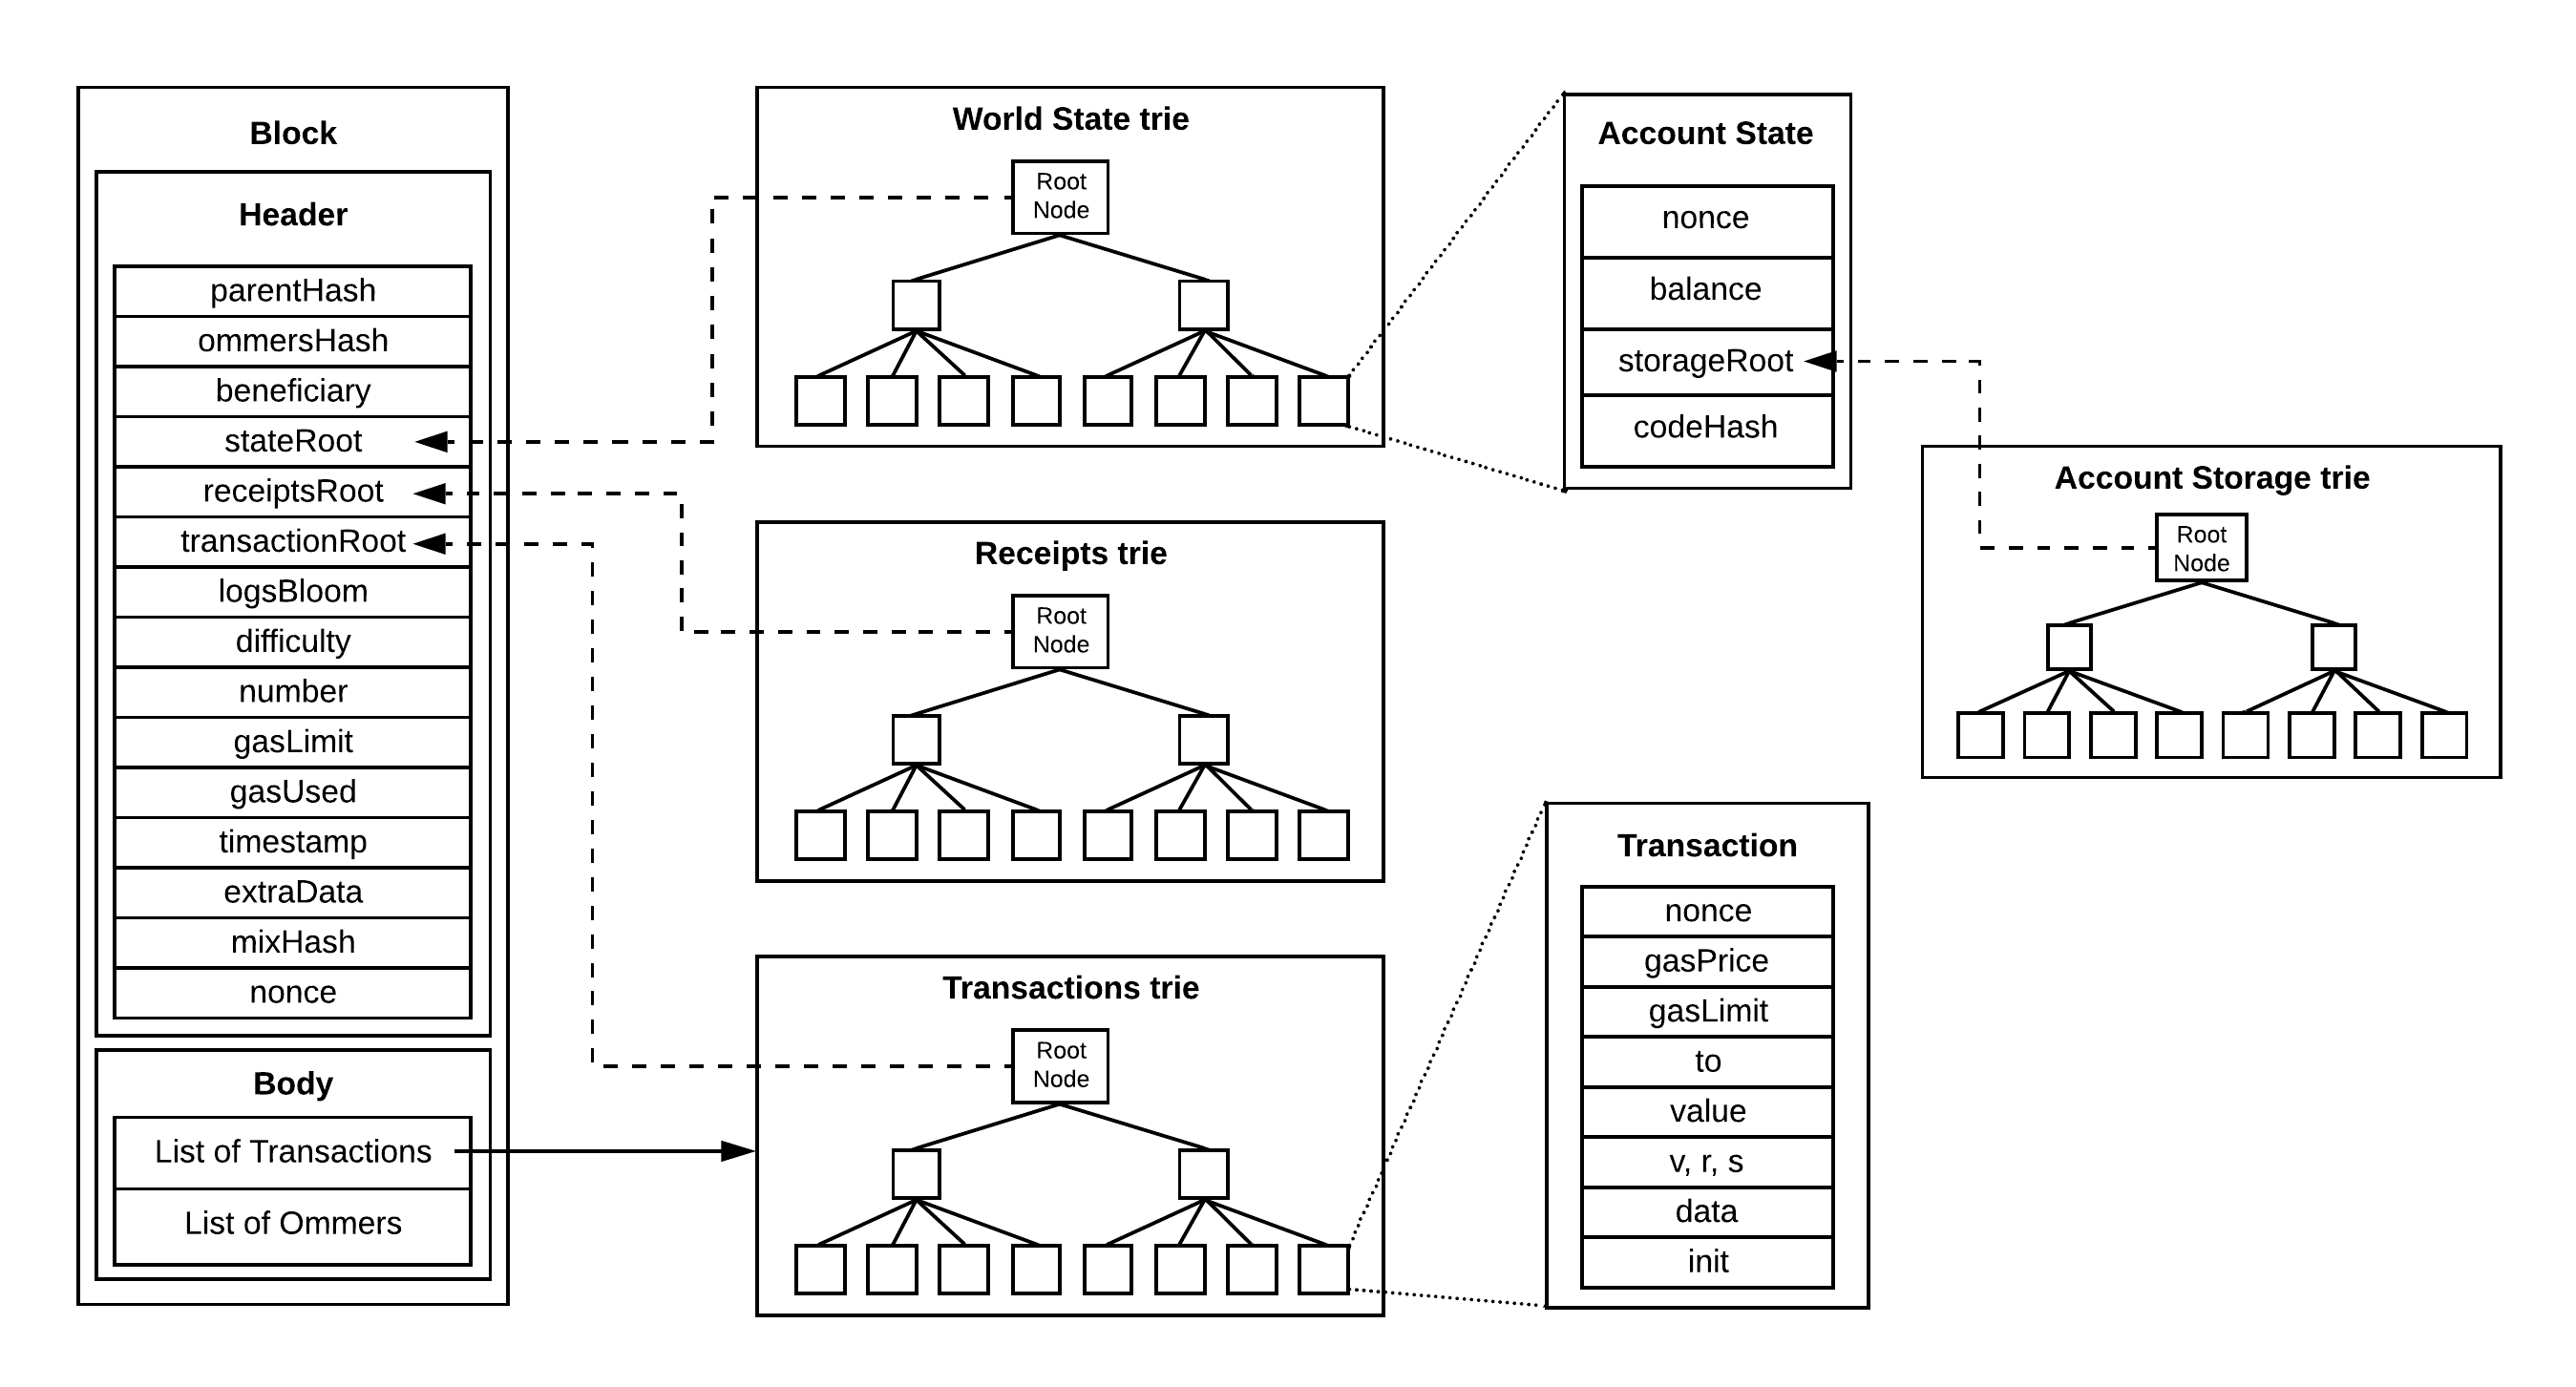
\includegraphics[height=10cm, width=14cm]{merkle_ptricia_trie.png}
  \centering
  \caption{Almacenamiento de Tries en los bloques}
  \label{fig:merkle-ptricia-trie}
\end{figure}

\paragraph{Trie de estados}

Existe un solo Trie de estado global en Ethereum y es constantemente actualizado. Este Trie posee un par de clave-valor para cada cuenta existente en Ethereum. La clave es un hash de 160 bits que identifica a la dirección pública de cada cuenta y el valor está dado por la codificación utilizando RPL de los valores de detalle de las cuentas que están conformados por los siguientes campos:

\begin{itemize}
  \item nonce: si la cuenta es de propiedad externa, este número representa la cantidad de transacciones enviadas desde la dirección de la cuenta. Si la cuenta es de contrato, el \textit{nonce} es el número de contratos creados por la cuenta (no es el mismo \textit{nonce} que se utiliza en el protocolo de consenso).
  \item balance: el balance en \textit{ether} que posee la cuenta.
  \item storageRoot: Es el \textit{hash} del Trie completo donde se guarda toda la información de los contratos; en caso de ser una cuenta común este dato es nulo.
  \item codeHash: Para las cuentas de contratos, es donde reside el \textit{bytecode} del mismo.
\end{itemize}

Como se puede observar existe un cuarto Trie, el Trie de almacenamiento, donde se guardan todas las variable e información relevante al contrato.  Este Trie se considera un sub-Trie del Trie de estado y la variable \textit{storageRoot} aloca el \textit{hash} del Trie de almacenamiento para esa determinada cuenta en un momento dado en el tiempo.

De estas cuatro variables que componen el estado de una cuenta, la única que no se modifica a lo largo del tiempo es la de \textit{codeHash}, que almacena el código fuente del contrato. Por lo tanto una vez que un contrato es guardado en la blockchain nunca más se podrá borrar o modificar.

Cabe destacar que las cuentas dentro del Trie de estado sólo son agregadas si son destinatario de al menos una transacción: no tendría sentido incluir cuentas sin balance o código interno para el caso de los contratos.

\paragraph{Trie de almacenamiento}
\label{bc_ethereum_storage_trie}

El Trie de almacenamiento, como se mencionó anteriormente, es donde residen los datos del contrato. Cada cuenta de Ethereum tiene su propio Trie de almacenamiento. Entonces en la variable \textit{storageRoot} de la cuenta dentro del Trie de estados se guarda el \textit{hash} del Trie de almacenamiento de la cuenta.

\paragraph{Trie de transacciones}

Cada bloque tiene una lista con todas las transacciones que posee. El orden de las transacciones es determinado por el nodo minero o validador, y una vez que se introduce el bloque dentro de la blockchain y es confirmado, esta lista de transacciones y sus posiciones nunca se podrá modificar. Por lo tanto, los pasos para buscar una transacción dentro del Trie de transacciones siempre van a ser los mismos y depende de la codificación e indexación RPL que se realiza al momento de la inclusión de las mismas.

\paragraph{Trie de recipientes}

Este Trie almacena datos de salida de las transacciones como el estado pos-transacción, el total de gas utilizado, el conjunto de \textit{logs} de transacciones (puede incluir eventos de contrato en caso de que existan) y el filtro de los \textit{logs}. Estos datos, al igual que las transacciones, no se modifican.

\paragraph{Transacciones}
\label{bc_ethereum_tx}

Las transacciones son la única componente que puede producir un cambio en el estado de la blockchain, ya sea mediante el envío de balance de una cuenta externa a otra, o la ejecución de un procedimiento dentro de un contrato. Las transacciones no son más que una cierta cantidad de parámetros específicos, empaquetados y firmados, y contienen los siguientes campos:

\begin{itemize}
  \item nonce: número de secuencia proveniente de la cuenta externa. Sólo tiene significado en el contexto de la dirección de envío. Es utilizado para evitar ataques de repetición.
  \item Precio del gas: el precio del gas que el originador está dispuesto a pagar.
  \item Límite de gas: la cantidad de unidades de gas que el originador está dispuesto a pagar.
  \item Recipiente: el destinatario de la transacción.
  \item Valor: la cantidad de \textit{ether} que se desea enviar al recipiente.
  \item Datos: datos binarios de longitud variable.
\end{itemize}

En un sentido estricto, el \textit{nonce} es un atributo de la dirección de origen; es decir, sólo tiene significado en el contexto de la dirección de envío. Sin embargo, el \textit{nonce} no se almacena explícitamente como parte del estado de una cuenta en la cadena de bloques. En su lugar, se calcula dinámicamente, contando el número de transacciones confirmadas que se han originado desde una dirección.

Antes de enviarla a la red se construye el paquete de datos que contiene los campos de la transacción y se serializa utilizando el esquema de codificación del Prefijo de Longitud Recursiva (RLP), que como se explicó anteriormente, Ethereum utiliza para codificar toda la información que reside dentro de la blockchain de una manera efectiva. Como resultado se obtiene un \textit{hash} que luego es firmado con la clave privada de la cuenta externa que origina la transacción.

\begin{figure}[H]
  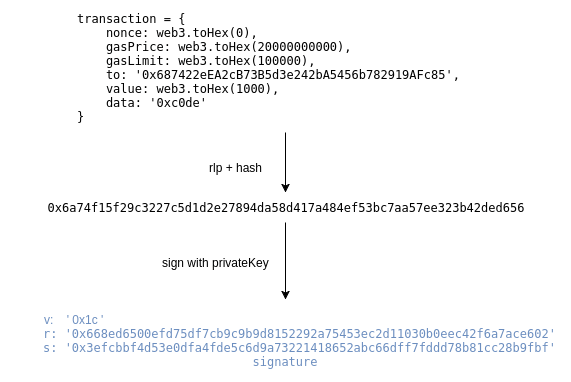
\includegraphics[height=10cm, width=14cm]{ethereum_transaction_signature.png}
  \centering
  \caption{Firma de una transacción en Ethereum}
  \label{fig:merkle-ptricia-trie}
\end{figure}

Una vez más se serializan todos los campos de la transacción más la firma digital para obtener el ID de la transacción. Este ID es un \textit{hash} de 256 bits y se utiliza para rastrear el estado o para consultar su estructura, ya sea mediante un explorador de bloques como lo es Etherscan\cite{Etherscan2018} o alguna herramienta que permita leer información de la blockchain.

\begin{figure}[H]
  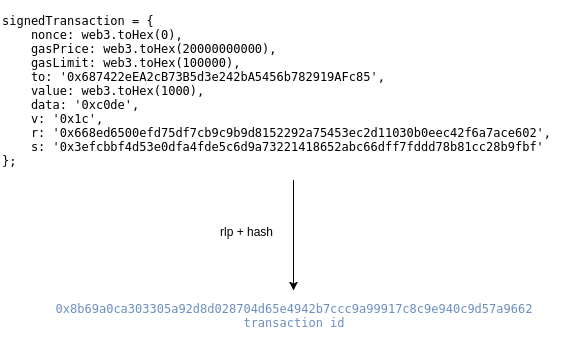
\includegraphics[height=10cm, width=14cm]{ethereum_transaction_txid.png}
  \centering
  \caption{Identificador de una transacción en Ethereum}
  \label{fig:merkle-ptricia-trie}
\end{figure}

Como se puede observar en el listado de campos de la transacción no se encuentra la dirección de la cuenta que origina la misma. Esto es debido a que dicha dirección se puede obtener a partir de la firma digital. También cabe destacar que dentro del cuerpo del mensaje sólo se envían los valores codificados sin los nombres de referencia. En general RLP no contiene ningún delimitador de campo o etiquetas, sino que se utiliza un prefijo que sirve para identificar la longitud de cada campo, con lo cual, cualquier dato más allá de la longitud definida pertenece al siguiente campo en la estructura.

Una vez empaquetada y firmada la transacción ya está lista para ser enviada a la red para que los mineros la validen y la agreguen a un nuevo bloque. El minero debe realizar las verificaciones pertinentes y, en particular, verificar si la cuenta que envió la transacción posee suficientes fondos para pagar la comisión que implica el envío de balance a otra cuenta o la ejecución de código dentro de un contrato. Y en estos cálculos, entra el concepto de gas.

\paragraph{Gas}
\label{bc_ethereum_gas}

El gas es el combustible de Ethereum. Es un concepto que va más allá del \textit{ether} pero a su vez están estrictamente ligados: no es una criptomoneda y tampoco se puede tener gas en una cuenta. El gas es una unidad de medida la cual determina la cantidad de cómputo que puede realizar una transacción dentro de la red, y así evitar ataques de denegación de servicios o bien bucles infinitos. Como se observa en el listado de parámetros de las transacciones existe: el límite de gas (gasLimit), que indica el máximo de unidades de gas que la transacción puede gastar, y a su vez, la cantidad de cómputo límite que la transacción podrá realizar. La cantidad de unidades de gas que requiere la ejecución de una instrucción de máquina dentro de la EVM está predeterminada en el ensayo amarillo de Ethereum (Yellow paper)\cite{wood2014ethereum} (por ejemplo, la cantidad de gas que consume la instrucción ADD es de 3 unidades).

Ahora bien, el uso del gas es para determinar una forma de pago al cómputo consumido por una transacción, por lo que lleva un valor asociado: el precio del gas (gasPrice), el cual, se paga en \textit{ether} y este precio responde a la volatilidad de la propia moneda y a la cantidad de tráfico que exista en la red; por lo general, el precio del gas se mantiene estable pero fluctúa levemente. Como se mencionó anteriormente, el precio del gas es establecido por la cuenta que envía la transacción y tiene ciertos márgenes de tolerancia: si el precio es relativamente más elevado que el precio real, la transacción se podría confirmar más rápido que si el valor es el mismo que el precio real y si está por debajo podría tardar más o nunca ser ejecutada.

El cómputo que se paga con el gas es realizado por los nodos mineros: estos ejecutan un programa cliente que es una máquina virtual con un cierto repertorio de instrucciones de máquinas Turing completa y son llamadas EVM (Ethereum Virtual Machine).

\paragraph{Máquina de estados (EVM)}
\label{bc_ethereum_evm}

La EVM es una de las piezas más importantes de Ethereum y es un motor de cómputo que provee una capa de abstracción para el procesamiento de operaciones y almacenamiento de datos, similar a lo que es la máquina virtual. Por lo tanto, la EVM es la encargada de almacenar y ejecutar el código de los contratos inteligentes. Los contratos son escritos en un lenguaje de alto nivel, como Solidity o Vyper y luego son compilados a un conjunto de instrucciones de \textit{bytecode} para ser ejecutados por la EVM. Las instrucciones de máquina que posee la EVM son denominados \textit{opcodes} y estos permite realizar operaciones como:

\begin{itemize}
  \item Aritméticas y lógicas bit a bit.
  \item Consultas de contexto de ejecución.
  \item Acceso a la pila, memoria y almacenamiento.
  \item De control de flujo.
  \item Registro, llamadas y otros operadores.
\end{itemize}

A continuación se detallarán algunos de los \textit{opcodes} para la ejecución de cálculos aritméticos:

\begin{minipage}{\linewidth}
  \begin{lstlisting}[frame=single, language=javascript, captionpos=b, caption=Ejemplo de optcodes, belowskip=1em, aboveskip=2em, label={lst:post_archivo}]
    ADD  //Suma los dos primero elementos de la pila
    MUL  //Multiplica los dos primero elementos de la pila
    SUB  //Resta los dos primero elementos de la pila
    DIV  //Division de enteros
    EXP  //Calculo exponencial
    SHA3 //Calcular el hash SHA256 de un bloque en memoria
  \end{lstlisting}
\end{minipage}

La EVM está compuesta por una memoria ROM y un estado de máquina (memoria volátil). La ROM es un código de programa inmutable que se carga junto al \textit{bytecode} del contrato inteligente y es necesario para la ejecución de los mismos, mietras que la memoria volátil está compuesta por las siguientes componentes:

\begin{itemize}
  \item \textbf{Pila:} La EVM es una máquina de pila, lo que significa que no realiza cálculos utilizando registros sino que usa una pila virtual. La pila tiene un tamaño máximo de 1024 y los elementos tienen un tamaño de 256 bits. La EVM es una máquina de palabras de tamaño de 256 bits debido a que esto facilita el esquema \textit{hash} SHA256 y los cálculos de curvas elípticas por los cuales se rige Ethereum.
  \item \textbf{Memoria:} La memoria es un espacio volátil que se puede direccionar por bytes de lectura y escritura virtual. Se utiliza para almacenar datos que serán utilizados durante la ejecución, como por ejemplo, para almacenar datos que van a ser utilizados como argumentos de una funcione interna. Dado que es un área de intercambio y en constante uso, cada ejecución de programa comienza con una memoria vacía: esto quiere decir que todas las ubicaciones de memoria se inicializan con valor cero.
  \item \textbf{Contador de programa:} Al igual que cualquier máquina que procesa operaciones, posee un contador de programa.
  \item \textbf{Gas disponible:} El conteo de unidades de gas disponibles para la ejecución de la operación.
  \item \textbf{Almacenamiento de cuenta:} Como se mencionó en \ref{bc_ethereum_storage_trie} los contratos almacenan toda su información en el Trie de almacenamiento. Es un espacio que se puede direccionar de palabras de lectura y escritura. A diferencia de la memoria, el almacenamiento es un área persistente. Es un mapeo clave-valor de $2^{256}$ espacios de 32 bytes cada una. Cabe aclarar que un contrato no puede leer ni escribir en ningún almacenamiento que no sea el suyo. Todas las ubicaciones se inicializan con valor cero. La cantidad de gas requerida para guardar los datos en el almacenamiento es una de las más altas entre las operaciones del EVM.

\begin{figure}[H]
  \includegraphics[height=10cm, width=14cm]{ethereum_evm_architecture.png}
  \centering
  \caption{Componentes de la EVM}
  \label{fig:merkle-ptricia-trie}
\end{figure}

A demás de las operaciones de máquina que puede realizar, la EVM también posee acceso al estado global de Ethereum, por lo que tiene al alcance información de lectura y escritura referida a las cuentas, transacciones y bloques. Todos los llamados a los contratos que requieran un cambio en el estado global de Ethereum son procesados por la EVM. Estos cambios tiene un costo asociado en base a la cantidad de operaciones máquina que son requeridos para realizar dicho cambio. Si el gas aportado por la transacción que pretende generar dicho cambio no es suficiente, la operación se revierte, aportando así una propiedad importante que concede la capacidad de finalizar procesamiento y poder evitar, por ejemplo, los ciclos infinitos. A su vez la EVM no posee acceso a los mecanismos de organización, manejo de proceso, interfaces de red o sistemas de archivos que están dentro del sistema operativo de la máquina anfitrión, puesto que la EVM fue pensada para ejecutar contratos inteligentes dentro de un entorno totalmente aislado, para evitar la manipulación y/o apoderamiento de los recursos de hardware.
\end{itemize}

\subsubsection{Algoritmos de Consenso}
\label{bc_ethereum_consensus}

En esta subsección se describirán las características de los algoritmos de consenso vinculados a la blockchain de Ethereum. En primer lugar se explicarán los algoritmos actualmente en uso y luego se mencionarán alternativas en desarrollo y para otro tipo de problemas.

Actualmente, el algoritmo de consenso usado en Ethereum se conoce como \textit{Ethash}, el cual es primordialmente un algoritmo de tipo \textit{Proof-of-Work}, muy similar a como se ha definido en su desarrollo teórico (\ref{bc_origins_hashcash}) y, en particular, en Bitcoin (\ref{bc_bitcoin_pow}); de hecho, el funcionamiento es prácticamente el mismo que este último: los nodos acumulan transacciones y validan los bloques, incrementando secuencialmente un valor \textit{nonce} hasta que el valor \textit{hash} final respecto al \textit{nonce} y al resto de los datos de la cabecera del bloque sea menor a un umbral (\textit{target}) -determinado por una dificultad autoajustada- para que la prueba de trabajo sea considerada válida.

 En Bitcoin, el consenso basado en \textit{PoW} requiere únicamente un trabajo de fuerza bruta a nivel de CPU. Aprovechando esto, y en plena efervescencia del Bitcoin, diversos fabricantes han diseñado y construido circuitos ASIC\footnote{Circuito Integrado para Aplicaciones Específicas} con el objetivo de optimizar y aumentar el \textit{hashrate} (tasa de \textit{hashes} probados por unidad de tiempo) requerido para la validación de bloques. Esto ha contribuido a desviar el poder de minado a un número reducido de nodos con el capital suficiente para invertir en este tipo de dispositivos y, en consecuencia, le ha restado cierta descentralización a la red.

 En busca de mitigar el problema enunciado, el algoritmo \textit{Ethash} presenta una implementación distinta, la cual, es deliberadamente mucho más demandante en términos de memoria y de entrada/salida. Es, en realidad, una versión mixta y mejorada de los algoritmos \textit{Dagger}\cite{buterin2013dagger} y \textit{Hashimoto}\cite{dryja2014hashimoto}. Básicamente lo que agrega es una estructura conocida como DAG, la cual es un grafo acíclico dirigido, y a partir de ella, se calcula el valor \textit{hash} final accediendo a una porción de esta estructura. La idea de que el validador constantemente tenga que acceder a una parte distinta e impredecible de dicho grafo hasta obtener el resultado final con el propósito de consumir exhaustivamente el ancho de banda de memoria, es la clave para combatir la proliferación de unidades ASIC y que una computadora normal pueda ser un justo competidor, para que de esta forma, pueda mantenerse mejor la propiedad de descentralización uniforme de la red.

 Más allá de las modificaciones y mejoras que se aplican constantemente sobre \textit{Ethash}, desde hace un tiempo -y no únicamente en \textit{Ethereum}- se ha estado analizando las problemáticas de los algoritmos \textit{PoW}, en particular, el desperdicio de energía en la búsqueda del \textit{hash} objetivo, con vistas de encontrar una alternativa. Una de las más sólidas es la de \textit{Proof-of-Stake} o Prueba-de-Participación: en lugar de invertir potencia de cómputo para validar bloques, lo que se hace es enviar una transacción especial a la red con una determinada cantidad de monedas, y en función de dicha cantidad, se obtienen mayores probabilidades de disponer del derecho de validar un bloque. La confianza de este método se sustenta en el hecho de que los participantes que más capital tienen, más interés tendrán en garantizar el correcto funcionamiento de la red. Y la principal ventaja que acarrea consigo es que ya no hará falta grandes caudales de procesamiento, ni por ende, desperdicio de energía, siendo un método mucho más rentable y eficiente. Dentro del marco de \textit{Ethereum} se ha estado desarrollando desde hace años un algoritmo de consenso \textit{PoS} (\textit{Proof-of-Stake}) bajo el nombre en clave \textit{Casper}\cite{zamfir2017casper}, el cual eventualmente reemplazará al actual algoritmo \textit{PoW} \textit{Ethash}. Cabe destacar que esta promesa es también una de las razones por las cuales los dispositivos ASIC no se han popularizado en esta red, dado que el paso hacia un consenso de tipo Prueba-de-Participación dejaría a los mismos inutilizables.

 Por último, para cerrar esta parte, se hará mención a un tipo de algoritmo de consenso bastante utilizado en blockchains privadas y de prueba, conocido como Prueba-de-Autoridad (o \textit{PoA}). En redes con este tipo de consenso se cuenta con un grupo reducido de nodos validadores que son los encargados de aprobar la integridad y la correctitud de los bloques. Además, estos nodos cuentan con una identidad pública, de forma tal que si se comportan maliciosamente, estos pueden ser expulsados de la red. La ventaja de este tipo de consenso es que las validaciones son sumamente veloces dado que no hay trabajo para invertir como en los métodos \textit{PoW} y el costo de malversar las transacciones es mucho mayor que en \textit{PoS} dado que la contraprestación es la identidad del nodo, algo que puede ser más fuerte y valioso que una determinada cantidad de monedas anónimas. Sin embargo, la mayor desventaja es precisamente la difusión de la identidad y ser parte de un grupo pequeño de validadores, que va en contra de la filosofía del anonimato y la descentralización, respectivamente, que son características inherentes a las blockchains, tal como fueron definidas originalmente. Por estas razones, los dominios en donde se emplea este tipo de consenso suelen ser redes pequeñas y acotadas, tales como las privadas -con cierto control jerarquizado- y las \textit{testnet} -las redes de tests para pruebas tempranas y rápidas de determinadas funcionalidades-. Un ejemplo muy concreto de \textit{testnet} con consenso \textit{PoA} es Kovan\cite{Kovan2019}, una red de prueba de \textit{Ethereum}.

\subsubsection{Contratos inteligentes}
\label{bc_ethereum_smart_contracts}

Para concluir con el marco teórico se describirá la noción de ``Contrato inteligente'', pieza clave en la implementación de la solución del problema enunciado en esta tesina.

El término ``Contrato inteligente'' fue acuñado por Nick Szabo (también creador de \textit{Bit Gold} , mencionado en \ref{bc_origins_bmbg}) en \textit{Formalizing and securing relationships on public networks}\cite{Szabo1997} donde, además, desarrolla de manera teórica y filosófica las razones por las cuales estos contratos inteligentes debieran ser la opción de facto para establecer relaciones seguras en la era digital, por medio de criptografía y protocolos de mensajes escritos en un lenguaje formal\footnote{Existe un primer borrador de lenguaje de definición de contratos inteligentes en \cite{Szabo2002}.}. En dicho artículo, se pone foco también en cuestiones como el anonimato y la descentralización -de hecho, hace mención de las \textit{Mix Networks} estudiadas en \ref{historia_descentralizacion} como mecanismo para lograr esto- para finalmente concluir que no es necesario una tercera parte activa que actúe como supervisor del cumplimiento del contrato.

Con la llegada de las blockchains -a partir de Bitcoin en 2009-, planteadas como plataformas seguras y descentralizadas para realizar operaciones, la idea de los contratos inteligentes volvió a cobrar interés. Más aún, se podría llegar a pensar que Bitcoin en realidad implementa un contrato universal para intercambiar monedas, y precisamente la idea que dio lugar al surgimiento de Ethereum fue el poder desacoplar de alguna forma la lógica de una operación determinada -por ejemplo, un intercambio de monedas- del contexto de ejecución inmutable y replicado en todos los nodos de la red.

En definitiva, si un contrato inteligente empaqueta la lógica de una operación de una manera rigurosa y consistente, entonces se podría definir un contrato como un programa cuyos efectos deben ser bien determinados y globalmente visibles y resguardados por toda la red. Para cumplir con estas condiciones, un contrato inteligente necesariamente debe ser inmutable -el código que implementa la lógica no puede cambiar- y determinístico -dada una transacción y un estado particular de la red, los efectos de la ejecución deben ser los mismos independientemente del contexto espacial o temporal de la misma-

En Ethereum, existen diversos lenguajes para definir contratos inteligentes. Pero lo más importante es que independientemente del lenguaje utilizado el código del contrato pueda compilarse al \textit{bytecode}\footnote{Conjunto de instrucciones primitivas.} de la EVM, desarrollada en \ref{bc_ethereum_evm}. En definitiva, la red Ethereum lo único que puede ejecutar es ese \textit{bytecode}.

Los contratos en Ethereum se crean por medio de una transacción especial encargada de desplegarlos. Como resultado, si el proceso es exitoso, se recibe la dirección pública del contrato para interactuar con él. Estas interacciones se realizan por medio del protocolo JSON-RPC\footnote{\url{https://github.com/ethereum/wiki/wiki/JSON-RPC}}, esto es, mediante mensajes en formato JSON\footnote{JavaScript Object Notation} se pueden hacer llamados remotos a procedimientos definidos dentro del contrato (RCP\footnote{Remote Procedure Call}). Tal como se mencionó en la subsección \ref{bc_ethereum_tx}, si una operación de un contrato va modificar el estado de la blockchain, dicha mutación necesariamente será reflejada por medio de una transacción, indicando el procedimiento y los parámetros del llamado. Dado que las transacciones son, por definición, atómicas, sólo se almacenan en la blockchain si la ejecución completa del procedimiento del contrato terminó exitosamente, de lo contrario, no se registra como tal (aunque sí se registra el intento fallido).

En cuanto al costo operativo de llamar a un procedimiento de un contrato, se consideran varias variables: en primer lugar, si dicha llamada crea una transacción se debe sumar el costo de comisión clásico. En este caso, asimismo, se tiene que adicionar el costo del gas insumido en la ejecución. Y, opcionalmente, podría haber un diferencial asociado a dicha función en particular, en cuyo caso, también se sumariza al costo total. Por otro lado, y en general, cualquier operación que realice simplemente una lectura de la blockchain sin alterarla, no tiene ningún costo, ni transaccional -ya que sin cambios en la blockchain, no hay transacciones-, ni de uso de gas -no se cobra en operaciones de lectura pura-, ni ningún otro extra.

Es importante destacar que dado que los contratos inteligentes no se pueden modificar una vez desplegados, su diseño tiene que ser cuanto menos excelente y muy bien testeado -por esta razón existen las \textit{testnets}-; de lo contrario, se tendrá en la blockchain un contrato deficiente que puede fallar, e incluso, ser atacado y provocar daños mayores.

Retomando la parte de lenguajes, si bien se ha expresado que existen varios, el más empleado hoy por hoy es \textit{Solidity}, probablemente por el simple hecho de ser el que presenta mayores similitudes con los lenguajes populares actuales, como Java y JavaScript. Por dicha razón, es el lenguaje que se usará para implementar el contrato inteligente que será parte de la solución del problema especificado en esta tesina.

\subsubsection{Recapitulación}

Se han mostrado los principales componentes de interés que constituyen a la blockchain de Ethereum, haciendo foco en sus particularidades necesarias para disponer de un modelo de cómputo general y distribuido, mucho más flexible y complejo que aquel mostrado en Bitcoin. A partir de estos cimientos, luego se ha explicado la idea de contrato inteligente como elemento e interfaz tanto para codificar como para ejecutar lógica y reglas de negocios personalizada.

Y con esto concluye el marco teórico. En base a todo lo expuesto, se verá en el siguiente capítulo -de implementación de la solución- cómo aplicar los fundamentos estudiados para diseñar y construir una alternativa descentralizada que posea, de forma inherente, mejores propiedades en cuanto a seguridad y disponibilidad.


\newpage
\section{Implementación de la solución}
\label{imp_solucion}

De acuerdo a lo enunciado previamente en el presente trabajo -ver \ref{recapitulacion_desc_problema}-, en esta propuesta debería evitarse el uso de un servicio central sobre el cual recaiga la confianza respecto a la integridad de los archivos.

A los efectos de poder demostrar la premisa precedente, se describirá en este apartado una posible solución al problema mencionado, empleando como vehículo, un pequeño sistema cuyo objetivo será el poder certificar archivos. Certificar un archivo implicará que el mismo, a partir de dicho acto, no podrá ser modificado de ninguna manera sin que esto altere la prueba de certificación. Hasta aquí, no varía mucho de cualquier servicio de certificación de inmutabilidad pero, como se dijo anteriormente, se desea evitar que el sistema dependa exclusivamente de un solo servidor que avale las certificaciones. Por esta razón, la novedad planteada aquí será la de distribuir esta certificación a una red blockchain pública -empleando Ethereum en este caso- con el fin de mitigar considerablemente el riesgo de ataque y malversación del servicio que brinda la certificación.

Certificar, desde un punto de vista más técnico y específico, será a los efectos prácticos establecidos en la presente sección, obtener una huella digital de un archivo por medio de una función de \textit{hash} de cifrado público segura, tal como se ha visto en \ref{funcion_una_sola_via}. Se ha usado, para la demostración, el algoritmo SHA-256 por cuestiones prácticas y algo arbitrarias, pero en si podría ser cualquier función en tanto garantice seguridad.

\subsection{Arquitectura de la aplicación}

Básicamente, la idea es disponer, dentro del sistema, de una parte que sea la interfaz con el usuario y/o aplicación cliente (de aquí en más, \textit{frontend}) la cual mínimamente va a recibir y mostrar los pedidos de las certificaciones. Por otra parte, se contará con la blockchain Ethereum que servirá de repositorio público y distribuido de las certificaciones (esto, podría considerarse \textit{backend}). Adicionalmente, dado que se trata de un servicio sobre archivos, habrá un servidor que aloje esta información. Es valioso destacar que no importa si dicho servidor es uno o muchos (centralizado o distribuido) dado que lo que interesa resguardar es la certificación del mismo y no el archivo en sí, es decir, su legitimidad entendiéndola como su inmutabilidad.

A continuación podrá verse un gráfico a muy alto nivel de la arquitectura del sistema:

\begin{figure}[H]
  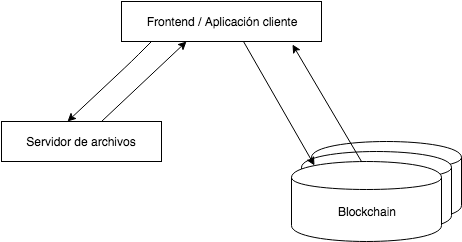
\includegraphics[height=6cm, width=12cm]{arq_sistema.png}
  \centering
  \caption{Arquitectura del sistema}
  \label{fig:arq-sistema}
\end{figure}

Lo que se intenta describir son los tres componentes básicos, es decir, el \textit{frontend}, el servidor de archivos y el \textit{backend} o blockchain, el cual necesariamente estará distribuido y replicado por su naturaleza intrínseca. Habrá interacciones bidireccionales entre el frontend y el servidor de archivos y entre el primero y la blockchain para las distintas operaciones a especificar. Y como se ha dicho anteriormente, opcionalmente el servidor de archivos podría estar replicado y las aplicaciones clientes también, si en futuro, por ejemplo, fueran aplicaciones móviles.

\subsubsection{Control propio de las transacciones}
\label{control_propio_transacciones}

Ahora bien, a partir de aquí se podrían elaborar muchas variantes. Una de ellas, que se ha discutido en un principio, es si introducir en la arquitectura presentada un \textit{backend} propio con control total del proveedor del servicio. Este nuevo planteo brinda algunos beneficios producto de colocar un punto en el medio del canal de comunicación entre los clientes y la blockchain:

\begin{enumerate}
  \item La cuenta para realizar las transacciones hacia la blockchain de Ethereum podría quedar a cargo del proveedor y no de los usuarios, lo cual podría hacer más cómodo y atractivo el servicio para estos últimos. Desde la perspectiva del proveedor, se puede recurrir a la instalación de uno o más nodos dedicados a minar (validar transacciones, muy similar a como se vio en \ref{bc_bitcoin_net_overview}) que ayuden a compensar el gasto transaccional generado por los usuarios.
  \item Podrían facilitarse cuestiones de autenticación y validación de usuarios de una manera más tradicional, y por ende, sencilla de implementar.
\end{enumerate}

A continuación se expondrá un gráfico ilustrativo de esta variante, similar al expuesto en la figura \ref{fig:arq-sistema}:

\begin{figure}[H]
  \includegraphics[height=7cm, width=12cm]{arq_sistema_conbackcentral.png}
  \centering
  \caption{Arquitectura del sistema con backend propio central}
  \label{fig:arq-sistema-conbackcentral}
\end{figure}

La principal desventaja de este modelo es que se deja expuesto un punto de centralización sobre un sistema distribuido, con lo cual, se vuelven a sumar problemas relacionados a la disponibilidad del servicio y a la confianza que, justamente, en una solución sobre la cual se justifica el uso de una blockchain se pretenden evitar. Con lo cual, por esta razón, se decidió trabajar con un modelo totalmente distribuido, es decir, con el frontend comunicándose directamente contra cualquier nodo de la blockchain, de manera tal que si uno de ellos cae, siempre se podrá acceder a otro que esté en funcionamiento y, por otro lado, con la ventaja de poder auditarse públicamente la información alojada en la misma y con la garantía de que la misma nunca fue, es y será alterada (ver \ref{bc_bitcoin_security})

\subsubsection{Resumen de la arquitectura propuesta}
\label{Resumen de la arquitectura propuesta}

Recapitulando lo expuesto en toda esta parte, el diseño de la aplicación consistirá de:

\begin{itemize}
  \item Frontend: una aplicación que brinde las operaciones necesarias al usuario como para listar, verificar y dar de alta certificaciones de archivos.
  \item Servidor de archivos: lugar donde residirán los archivos. Debería proveer por archivo una huella y una identificación unívoca y anónima.
  \item blockchain (Backend): el corazón de la aplicación, en donde se persistirán y distribuirán las huellas de los archivos.
\end{itemize}

\subsection{Especificación de las operaciones}

A continuación se describirán las principales operaciones que permitirá realizar la aplicación. Como se ha dejado establecido, se deberán proveer por lo menos dos casos de uso:

\begin{enumerate}
  \item  La posibilidad de dar de alta certificaciones de archivos
  \item  La posibilidad de listar y verificar las certificaciones de los archivos
\end{enumerate}

\subsubsection{Alta de certificación}
\label{alta_certificacion}

A continuación, se mostrará el diagrama de secuencia pertinente a la operación de alta de una certificación junto con una breve explicación paso a paso:

\begin{figure}[H]
  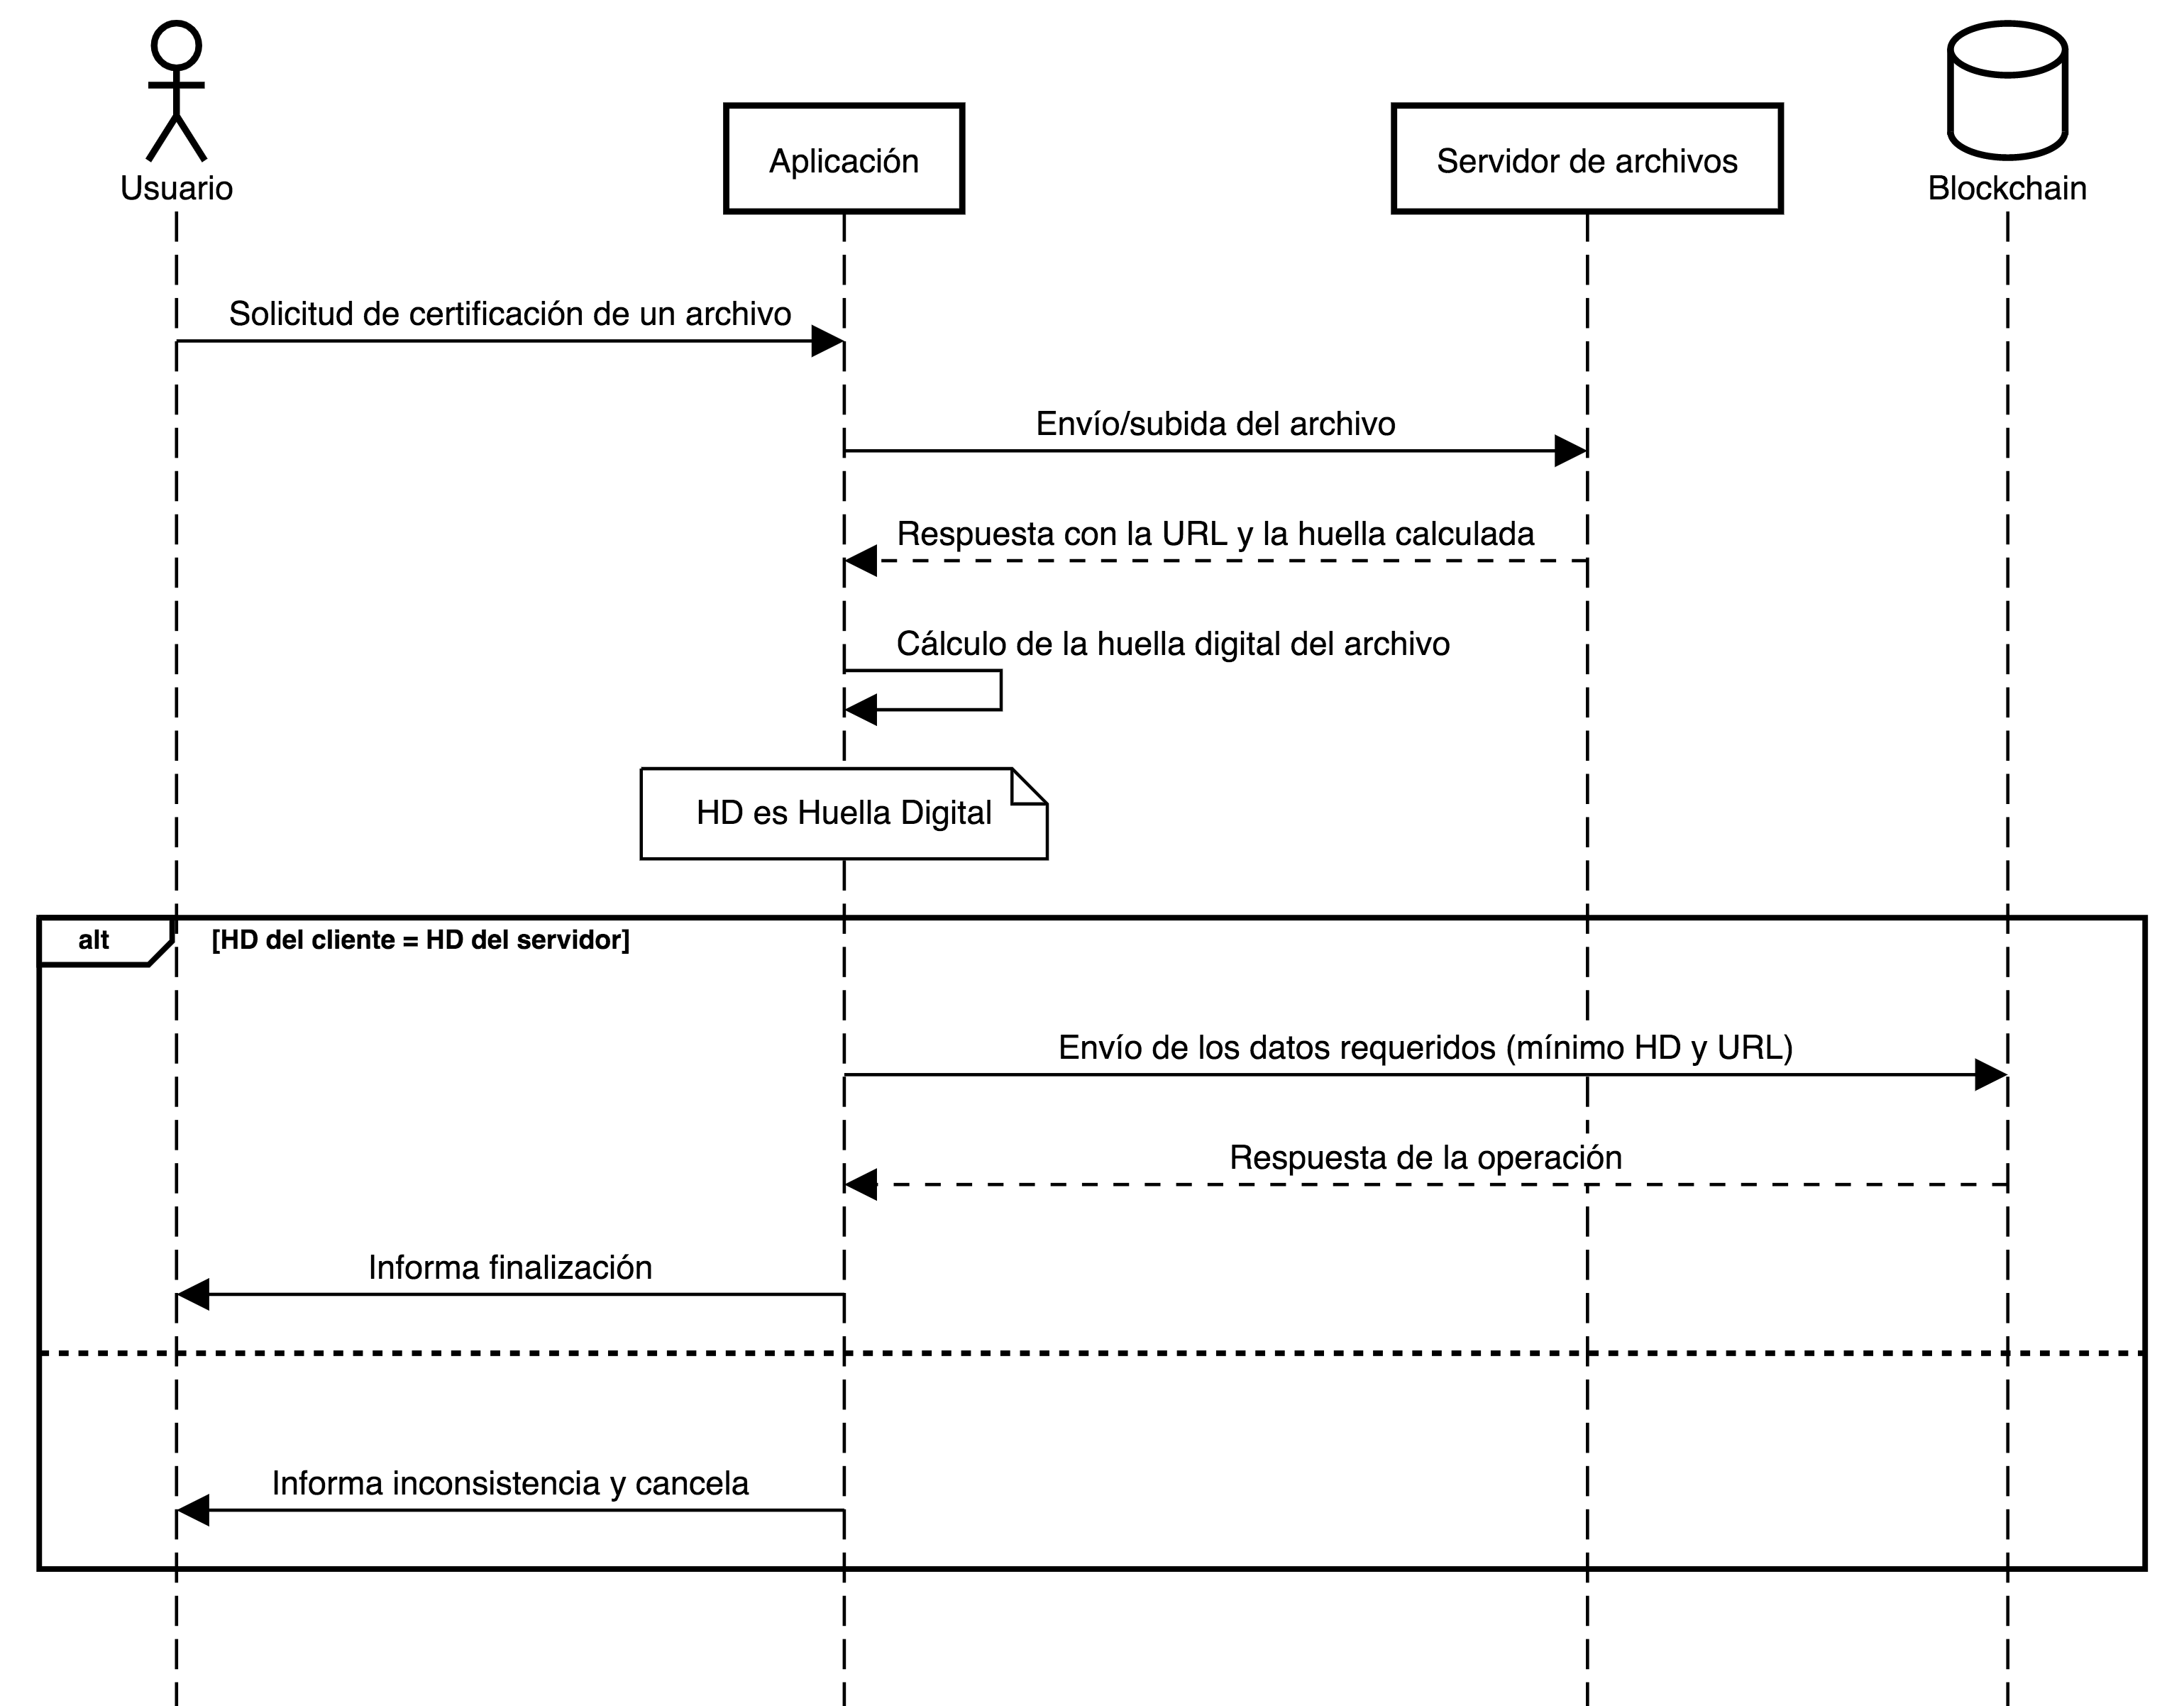
\includegraphics[height=12cm, width=14cm]{upload_certificado_diagrama_secuencia.png}
  \centering
  \caption{Operación alta de certificación}
  \label{fig:upload-certificacion-diagrama-secuencia}
\end{figure}

El primer paso, lógicamente, es solicitar desde el \textit{Frontend} el archivo a certificar. Esto es lo mínimo indispensable como para que esta operación funcione correctamente. Adicionalmente es posible solicitar más información, lo cual se analizará en el apartado \ref{datos_guardar_blockchain}.

El archivo se transfiere hacia el servidor de archivos donde será alojado para futuras consultas y/o descargas. Si esta operación es exitosa, la respuesta que recibirá el \textit{Frontend} será la URL del recurso almacenado y la huella digital del mismo calculada en aquel servidor.

Luego se calcula la huella digital del archivo que ya se encuentra residente en la aplicación \textit{Frontend} y se compara dicha huella con aquella que fue recibida desde el servidor. Si ambas coinciden, se procede con la operación; de lo contrario, se cancela y se informa al usuario. La razón de hacer esta comprobación es para suministrarle al circuito una capa de seguridad adicional en el tramo de transferencia del archivo desde el \textit{Frontend} hacia el servidor de archivos, es decir, si por alguna razón alguien o algo ya sea de manera intencionada o fortuita interfiere en dicho canal de comunicación hacia un componente centralizado (recordar que el servidor de archivos puede ser único), entonces esta verificación servirá para detectar inconsistencias o anomalías en este paso.

Si en este punto todo se encuentra en orden, entonces ahora sí, se procede a la transferencia de la información hacia la blockchain. Nuevamente, lo mínimo que se debería transferir es la huella digital y el identificador del archivo. Opcionalmente se podría empaquetar en dicha transacción otros metadatos útiles para la posterior identificación de la operación de certificación. Cabe destacar que, generalmente, esta funcionalidad puede demorar bastante más que el resto dadas las características inherentes de la blockchain tales como la espera de confirmaciones de algunos nodos y ejecución del contrato inteligente (ver \ref{bc_bitcoin_net_overview} y \ref{bc_ethereum_gas})

Finalmente, si el guardado en la blockchain fue exitoso, se informa al usuario que la operación fue realizada correctamente, y con esto, concluye la operación de certificación.

\subsubsection{Datos a almacenar en la blockchain}
\label{datos_guardar_blockchain}

La idea en esta sección es analizar sucintamente qué datos podrían insertarse dentro de la blockchain, más allá de la indispensable huella digital.

Pero antes, se podría evaluar si, además o en lugar de la huella digital, se podría almacenar el archivo entero dentro de ella. Para los propósitos de este trabajo, dicha opción no resulta conveniente por las siguientes desventajas técnicas y de seguridad que subyacen:

\begin{enumerate}
  \item Subir un archivo a la blockchain podría, en general, exceder los límites de una transacción simple y, además, en el caso particular de la blockchain de Ethereum, también entra en juego la variable del \textit{gas} que tiene un límite máximo por transacción y por bloque (ver \ref{bc_ethereum_gas}); aun ignorando todo esto, sería también potencialmente costoso dado que, justamente, el \textit{gas} insume dinero.
  \item No sería posible subir archivos a una blockchain pública con información sensible. Respecto a esto, cabe destacar que siempre se evitará mostrar información o contenido respecto al archivo. Una vez más, el objetivo es únicamente demostrar que el archivo, a partir de un determinado momento, tiene cierto contenido identificado a través de un sello/huella y, por ende, no podrá cambiar.
\end{enumerate}

Entonces, además de la huella digital, ¿qué otros datos podrían considerarse guardar?

En primer lugar se podría pensar, tal vez, en incluir como dato esencial el momento en el cual se registra la certificación en la blockchain, es decir, una fecha/hora o \textit{timestap} de la operación. Esta afirmación no sólo es válida sino que también es insoslayable: la certificación, justamente, garantiza inmutabilidad del recurso certificado desde un momento determinado, con lo cual, este dato debería ser obligatorio para que esta operación tenga sentido. No obstante, las transacciones -más precisamente los bloques- que se realizan en cualquier arquitectura de tipo blockchain -y en particular, en Ethereum- registran siempre el momento en el cual son creadas, con lo cual, implícitamente esta información siempre está disponible (ver \ref{bc_bitcoin_components} y \ref{bc_ethereum_data_layer}). Como contraargumento se podría mencionar que este dato, devenido de la creación del bloque y la transacción contenida en él, no es exacto puesto a la demora que transcurre entre el momento en el cual se solicita el registro de la certificación en el \textit{Frontend} y el momento en donde efectivamente se confirma la transacción en la red de blockchain. En caso de ser sumamente necesario contar con dicha exactitud se podría registrar aquel momento como dato adicional, solicitándolo desde algún servicio externo que brinde certificación de tiempo en los primeros pasos de la certificación, es decir, antes de transferir el archivo al servidor de archivos.
En segundo lugar podrían enviarse datos referentes al usuario del sistema y/o propietario del archivo a certificar, con el propósito de informar, justamente, quién solicitó dicha operación.
Adicionalmente, otro dato que podría ser útil en algunos contextos es la geolocalización, ya sea registrando las coordenadas o mediante dirección IP. Esto permitiría saber dónde se solicitó la certificación.
Y por último, se podría incluso pensar en dejar un campo libre donde el usuario puede comentar o registrar cualquier información pertinente al proceso de certificación para que quede registrado en la blockchain de forma permanente.

\subsubsection{Listado de certificaciones}
\label{listado_certificaciones}

La operación que lista las certificaciones realizadas en el sistema se describe gráficamente de la siguiente manera:

\begin{figure}[H]
  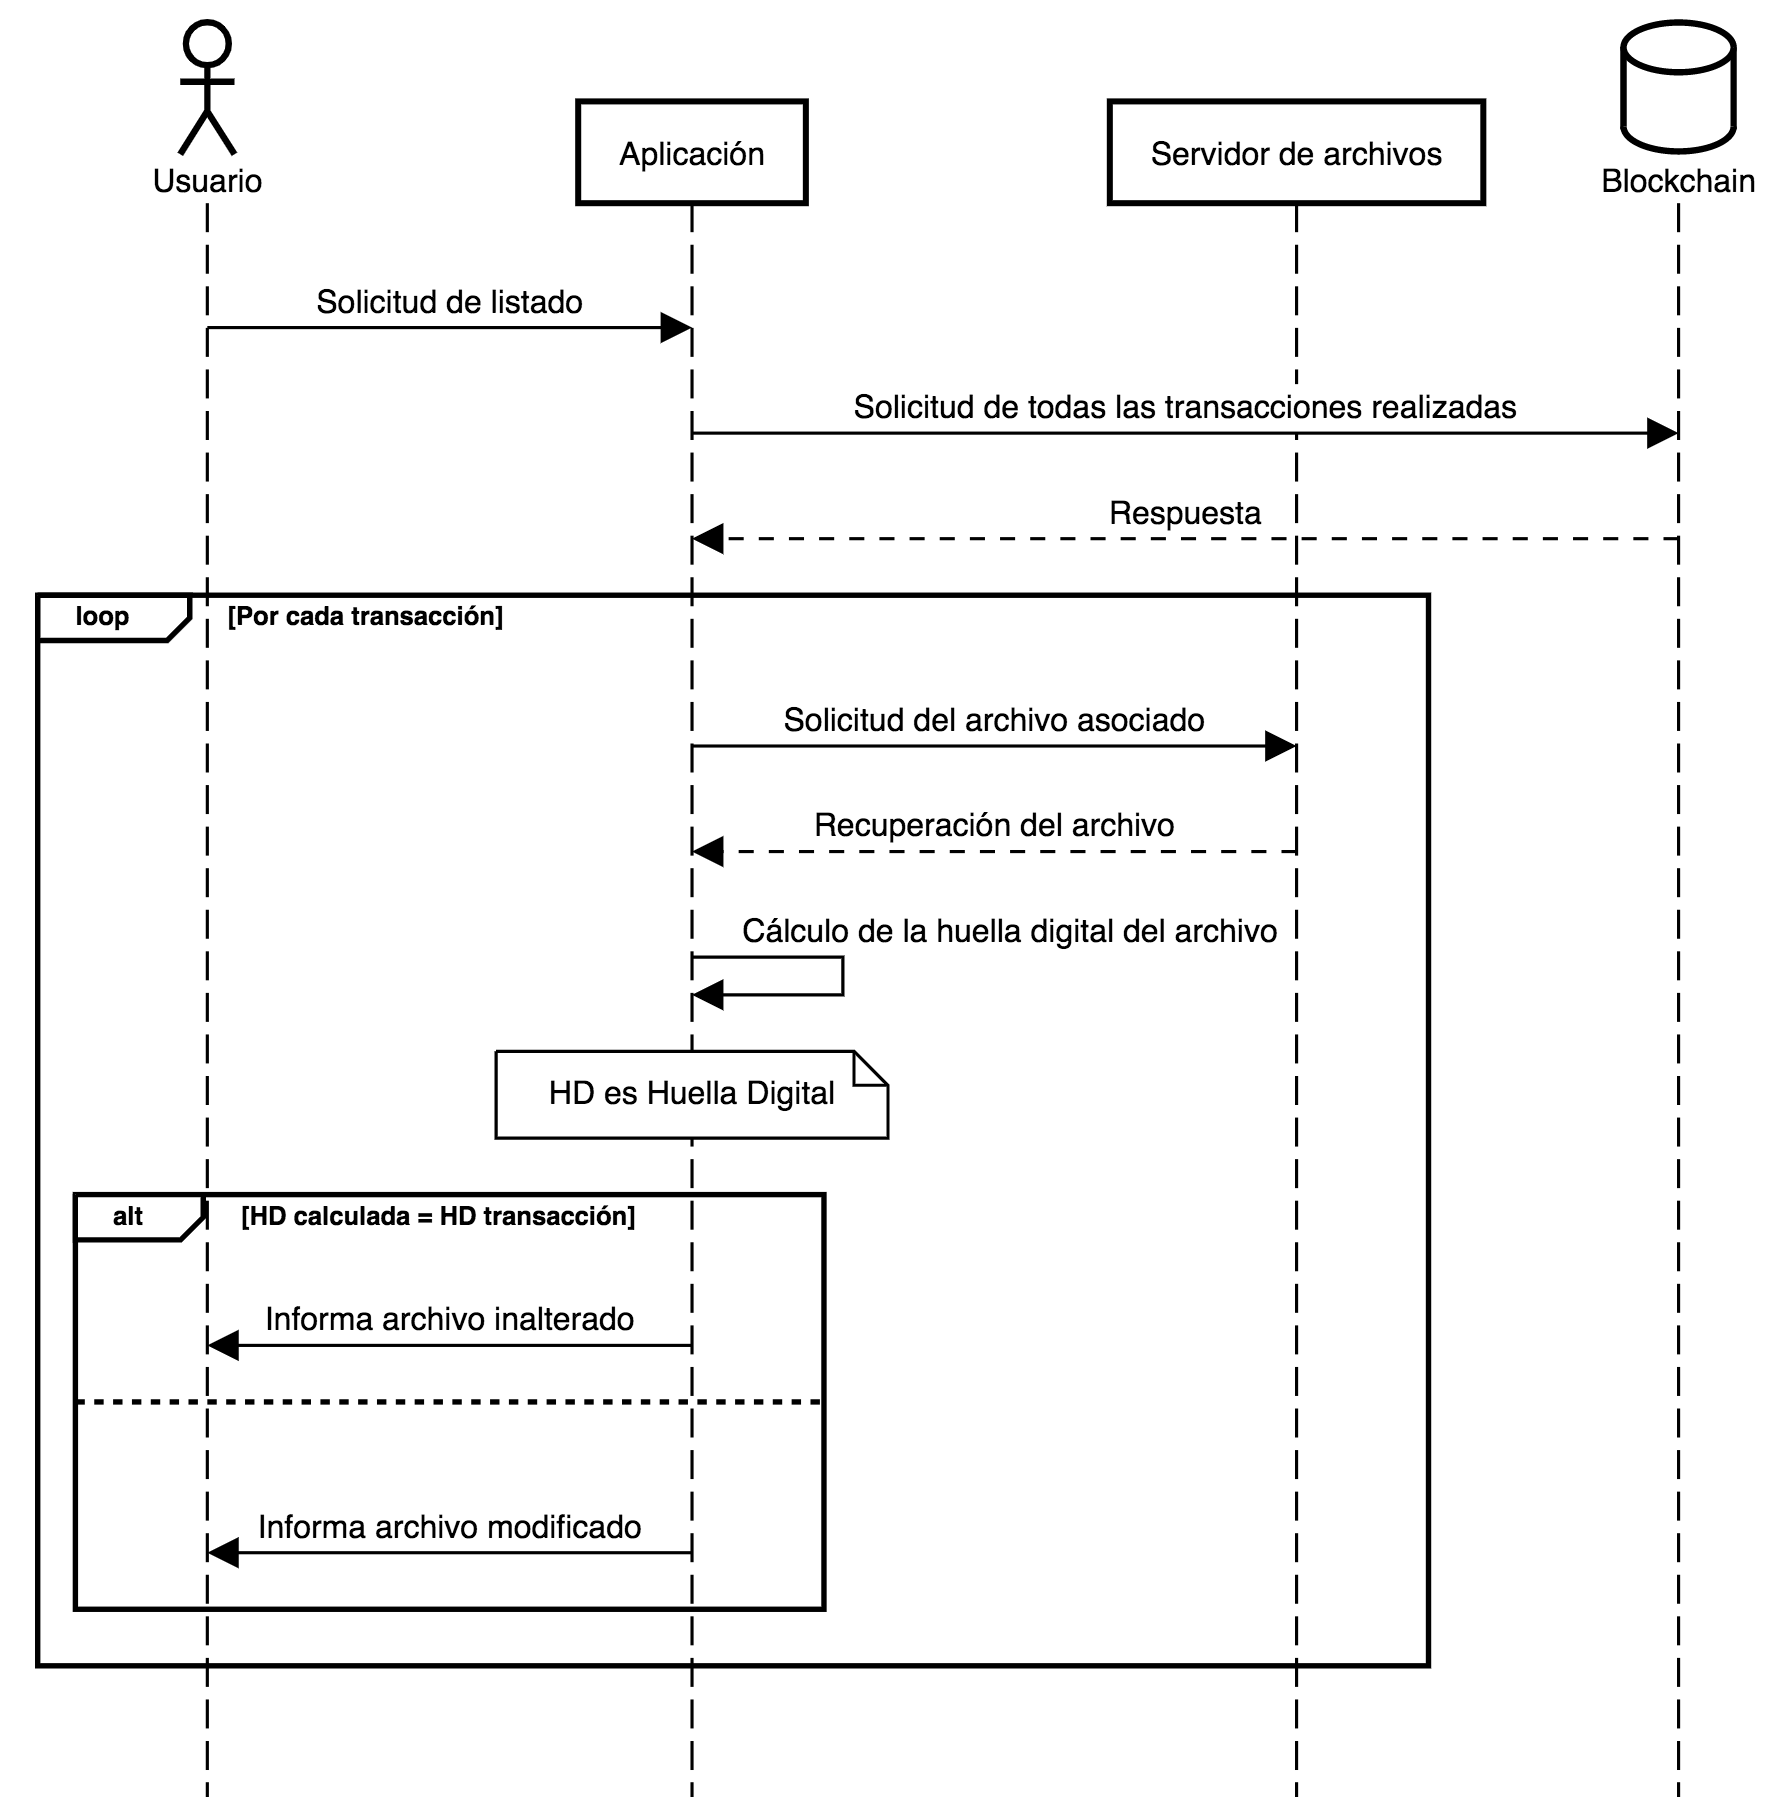
\includegraphics[height=14cm, width=14cm]{listado_certificaciones_diagrama_secuencia.png}
  \centering
  \caption{Operación listado de certificaciones}
  \label{fig:listado-certificaciones-diagrama-secuencia}
\end{figure}

Lo primero que transcurre en esta operación es la solicitud de los datos procedentes de las transacciones que se hicieron sobre la blockchain. Una vez que se recuperan dichas transacciones se procede a obtener, para cada una de ellas, la información del archivo tal como está en ese momento desde el servidor de archivos, a través del identificador que fue registrado durante la certificación, en conjunto con la huella digital.  Una vez realizado esto, se calcula la huella digital de cada uno en el \textit{frontend}, o dicho de manera equivalente, localmente, y se la compara contra la huella digital alojada en la transacción obtenida: si son iguales, significa que no hubo alteraciones desde aquel momento; de lo contrario, entonces el archivo, por alguna razón -ya sea por imperfecciones en la red, en el almacenado del archivo o mediante terceros de manera intencionada o involuntaria-, se vio adulterado.
Toda esta información es mostrada al usuario para que así pueda informarse acerca del estado de integridad de cada uno de los archivos certificados.

\subsection{Implementación de las operaciones}

En esta sección se dará un pantallazo general respecto a la implementación del sistema especificado previamente. Se arrancará primero con el \textit{backend} que estaría representado por el contrato inteligente desplegado en la blockchain de Ethereum, y posteriormente, se verán las implementaciones de las diferentes operaciones que pueden realizarse desde el \textit{frontend}.

\subsubsection{Contrato inteligente (\textit{backend})}

Como se explicó en los capítulos \ref{bc_ethereum_smart_contracts} y \ref{bc_ethereum_evm}, los contratos inteligentes son fragmentos de código que son interpretados y ejecutados por las máquinas virtuales que residen en los nodos mineros de la red, en este caso, Ethereum. Estos están compuestos por un estado -representado mediante variables globales- y funciones que contiene lógica programable que permiten la manipulación de dicho estado -lectura y escritura-. Para programar los contratos inteligentes se pude utilizar distintos tipos de lenguajes, para este caso se decidió utilizar \textit{Solidity}\cite{Solidity2019}. La elección fue tomada teniendo en consideración los siguientes puntos:

\begin{itemize}
  \item Solidity fue diseñado específicamente para la plataforma Ethereum.
  \item La mayor parte de los componentes y librerías que circulan en la red están realizados en Solidity.
  \item Existe gran cantidad herramientas creadas para la construcción, verificación y prueba de los contrato inteligentes desarrollados sobre Solidity.
  \item Es fácil de aprender y utilizar.
\end{itemize}

Una vez dicho esto, se procede al análisis del código y las estructura del contrato, comenzando con las variables de estado necesarias para almacenar la información que compone a la huella digital y luego las funciones que aportan el comportamiento lógico.

\paragraph{Variables de estado del contrato (\textit{backend})}

Solidity provee diferentes tipos de datos y para representar la huella digital se utilizará el tipo \textit{byte} que es un arreglo de longitud dinámica y almacena bytes. Como la huella digital es un dato hexadecimal de 256 bits se podría alocar en un arreglo con una longitud de 32 bytes. Este tipo de arreglo dinámico es especial debido a que existe la posibilidad de declarar dichos arreglos de longitudes fijas. Una diferencia práctica importante entre los arreglos dinámicos y fijos es que los arreglos de longitud fija se pueden usar en argumentos de función para pasar datos o retornar datos fuera del contrato. El tipo \textit{bytes} de longitud variable también se puede utilizar como argumento de funciones, pero solo para uso interno (dentro del mismo contrato), porque la interfaz llamada ABI no permite -al menos por el momento- tipos de longitud variable como retorno de funciones externas. Por lo tanto se utilizará el tipo de dato \textit{bytes32} para almacenar la huella digital.

\begin{minipage}{\linewidth}
  \begin{lstlisting}[frame=single, language=javascript, captionpos=b, caption=Tipo de dato NotarizedFile, belowskip=1em, aboveskip=2em, label={lst:post_archivo}]
    struct NotarizedFile {
        string name;
        string fileUrl;
        uint256 timestamp;
    }
  \end{lstlisting}
\end{minipage}

La palabra reservada \textit{struct} se utiliza para crear estructuras (tipo producto)  de datos definidos por el usuario; su comportamiento y declaración es similar a cualquier lenguaje de programación. En este caso se utilizará para crear la estructura \textit{NotarizedFile} que contendrá los campos referidos a los metadatos de la huella digital:

\begin{enumerate}
  \item name: El nombre del usuario que realizará la certificación.
  \item fileUrl: La dirección URL del lugar físico donde residirá el archivo.
  \item timestamp: La marca de tiempo, la cual determinará la fecha y hora en la que se publicará el bloque de la transacción.
\end{enumerate}

Como se mencionó anteriormente, los datos que componen esta estructura de datos podría ser mayor, dependiendo de las necesidades de la aplicación.

\begin{minipage}{\linewidth}
  \begin{lstlisting}[frame=single, belowskip=1em, aboveskip=2em,  language=javascript, captionpos=b, caption=Variable de estado notarizedFiles, label={lst:post_archivo}]
    mapping (bytes32 => NotarizedFile) public notarizedFiles;
  \end{lstlisting}
\end{minipage}

Una estructura de datos similar a lo que sería una tabla hash clave-valor, es decir que para cada clave del \textit{mapping} existe un valor asociado. Este tipo de dato permite realizar el enlace de la estructura \textit{NotarizedFile} detallada anteriormente y la huella digital del archivo que se representará como un tipo de dato \textit{byte32}.

\begin{minipage}{\linewidth}
  \begin{lstlisting}[frame=single, belowskip=1em, aboveskip=2em,  language=javascript, captionpos=b, caption=Variable de estado filesByHash, label={lst:post_archivo}]
    bytes32[] public filesByHash;
  \end{lstlisting}
\end{minipage}

Un arreglo de tipo \textit{bytes32} para almacenar las huellas digitales de todos los archivos certificados. Esta variable nos permite consultar el número total de archivos certificados por el sistema para obtener un dato estadístico o bien para iterar sobre los mismos.

\paragraph{Funciones del contrato (\textit{backend})}

Dentro de un contrato pueden existir dos tipos de funciones, las que modifican el estado del mismo -escritura- y las que consultan el estado -lectura-. Las que modifican el estado se ejecutan mediante la creación de transacciones y como se mencionó en el apartado \ref{bc_ethereum_smart_contracts} las transacciones tiene un costo, debido a que las mismas quedan alojadas en la blockchain. El costo de las transacciones depende de la cantidad de parámetros enviados y la cantidad de líneas que posee la función y se paga con la criptomoneda nativa de la blockchain donde se ejecuta, en este caso \textit{ether}. Por otro lado existen las funciones de lectura, las cuales no modifican el estado del contrato, por este motivo es que el costo de estas funciones es cero. A continuación se detallarán cada una de las funciones que componen al contrato inteligente de la tesina:

\begin{minipage}{\linewidth}
  \begin{lstlisting}[frame=single, belowskip=1em, aboveskip=2em,  language=javascript, captionpos=b, caption=Función addFile, label={lst:post_archivo}]
    function addFile(
      bytes32 _notarizedHash,
      string calldata _name,
      string calldata _fileUrl
    ) external returns(bool) {
      require(
        bytes(_name).length != 0, "El nombre es requerida"
      );
      require(
        bytes(_fileUrl).length != 0, "La URL es requerida"
      );
      require(
        _notarizedHash.length != 0, "El hash es requerido"
      );
      require(
        notarizedFiles[_notarizedHash].timestamp == 0,
        "El archivo fue agregado previamente"
      );

      notarizedFiles[_notarizedHash].name = _name;
      notarizedFiles[_notarizedHash].fileUrl = _fileUrl;
      notarizedFiles[_notarizedHash].timestamp = now;
      filesByHash.push(_notarizedHash);

      emit FileAdded(_notarizedHash);
      return true;
    }
  \end{lstlisting}
\end{minipage}

La función \textit{addFile} no se puede ser accedida internamente, sólo externamente. Esto es debido a la palabra reservada \textit{external} en la línea 5 que otorga dicho comportamiento, a estas componentes de declaración de funciones se las llama \textit{modificadores de acceso}. La función permite básicamente dar de alta una nueva certificación con la huella digital y los metadatos correspondientes a la misma. Esto conlleva a un cambio de estado y por lo tanto el usuario debe pagar por dicha ejecución. En un primer paso se puede observar que se verifica mediante el uso de \textit{require} que los datos recibidos por paramentos no sean igual a cero, como es así la longitud de la huella digital. Solidity usa estructuras de control de excepciones para el manejo de errores y así evitar que, por ejemplo, el usuario que ejecuta una función de un contrato inteligente no envíe parámetros erróneos. Entonces si la condición dada dentro de \textit{require} es falsa, la transacción es revertida por completo, provocando las siguientes dos consecuencias: el estado del contrato vuelve al mismo valor que poseía antes de ser ejecutada la función y se devuelve al usuario la misma cantidad de \textit{ether} que utilizó para ejecutar dicha función.
Una vez corroborado que los parámetros son válidos se procede al almacenamiento de la información: como se puede ver de la línea 20 a la 22 se almacenan en el \textit{mapping} \textit{notarizedFiles} como valor los metadatos y como clave la huella digital y en la línea 23 se agrega la huella al arreglo de huellas. Por último se emite el evento \textit{FileAdded} y se retorna el valor true para confirmar el éxito de la transacción. Los eventos, en \textit{Solidity}, son la forma de alertar a las aplicaciones descentralizadas que se produjo un cambio en el estado de un contrato.

\begin{minipage}{\linewidth}
  \begin{lstlisting}[frame=single, belowskip=1em, aboveskip=2em,  language=javascript, captionpos=b, caption=Función removeFile, label={lst:post_archivo}]
    function removeFile(bytes32 _notarizedHash) external {
        require(
            _notarizedHash.length != 0,
            "El hash es requerido"
        );
        require(
            notarizedFiles[_notarizedHash].timestamp != 0,
            "El archivo no existe"
        );

        notarizedFiles[_notarizedHash].name = "";
        notarizedFiles[_notarizedHash].fileUrl = "";
        notarizedFiles[_notarizedHash].timestamp = 0;
        _removeHash(_notarizedHash);

        emit FileRemoved(_notarizedHash);
    }
  \end{lstlisting}
\end{minipage}

La función \textit{removeFile} también sólo puede ser accedida externamente y elimina un registro de una huella digital dentro del contrato. Se sabe que debido a la naturaleza de la blockchain los datos ingresados dentro de la misma son inmutables, por lo tanto esta función tiene como objetivo demostrar que la única forma de borrar información en un contrato es realizando un borrado lógico. Para ello igual que en la función anterior se verifica que los parámetros que recibe la función sean válidos y luego se procede al borrado. El proceso consiste en darle valores por defecto a los campos de los metadatos asociados a la huella que se desea borrar. Como segundo paso se ejecuta la función \textit{\_removeHash} que elimina la huella del arreglo de huellas, su proceso se detallará más adelante. Y como paso final se emite el evento para alertar a las aplicaciones descentralizadas.

\begin{minipage}{\linewidth}
  \begin{lstlisting}[frame=single, belowskip=1em, aboveskip=2em,  language=javascript, captionpos=b, caption=Función \_removeHash, label={lst:post_archivo}]
    function _removeHash(bytes32 _hash) private {
        uint length = filesByHash.length;
        for (uint i = 0; i < length; i++) {
            if (filesByHash[i] == _hash) {
                filesByHash[i] = filesByHash[length-1];
                filesByHash.length--;
                return;
            }
        }
    }
  \end{lstlisting}
\end{minipage}

La función \textit{\_removeHash} posee el modificador de acceso \textit{private} lo cual indica que sólo permite ser ejecutada internamente a través de otra función que pertenezca al contrato donde está declarada. Tiene como fin eliminar una huella digital dentro del arreglo de huellas. Consiste en la búsqueda de la posición de la huella a eliminar y una vez ubicada se procede a reemplazar la huella de esa posición por la de la última posición. Por último se reduce el tamaño del arreglo en uno. Igual que en la función \textit{removeFile} el borrado es lógico y si se quiere obtener los valores de la huella digital eliminada, sólo se tiene que observar cómo está compuesta la transacción que originó dicho registro.

\begin{minipage}{\linewidth}
  \begin{lstlisting}[frame=single, belowskip=1em, aboveskip=2em,  language=javascript, captionpos=b, caption=Función getFileByHash, label={lst:post_archivo}]
    function getFileByHash(bytes32 _notarizedHash)
        external
        view
        returns(string memory, string memory, uint256)
    {
        require(_notarizedHash.length != 0, "El hash es requerido");
        require(notarizedFiles[_notarizedHash].timestamp != 0, "El archivo no existe");

        NotarizedFile memory notarizedFile = notarizedFiles[_notarizedHash];
        return (
            notarizedFile.name,
            notarizedFile.fileUrl,
            notarizedFile.timestamp
        );
    }
  \end{lstlisting}
\end{minipage}

En la función \textit{getFileByHash} se puede observar en la línea 3 que se presenta la palabra reservada \textit{view} en la declaración de la misma. Esto indica que esta función no va a realizar cambios de estado, solo operaciones de lectura. Esta función permite obtener los metadatos de una huella digital pasada como parámetro: primero realiza las verificaciones sobre el parámetro de entrada y luego retorna los metadatos correspondientes. El valor de esta ejecución es 0 y no se realiza una transacción para obtener los datos.

\begin{minipage}{\linewidth}
  \begin{lstlisting}[frame=single, belowskip=1em, aboveskip=2em,  language=javascript, captionpos=b, caption=Función getNumberOfFiles, label={lst:post_archivo}]
    function getNumberOfFiles() external view
        returns(uint256)
    {
        return filesByHash.length;
    }
  \end{lstlisting}
\end{minipage}

La función \textit{getNumberOfFiles} retorna la cantidad de huellas certificadas hasta el momento de la ejecución. Es una función externa y no realiza modificaciones en el estado del contrato.

En conclusión, teniendo en cuenta que los contratos una vez desplegados en la blockchain no se pueden modificar, se tuvo en cuenta ciertas prácticas que agilizan el proceso de codificación y aportan seguridad al mismo, tales como:

\begin{itemize}
  \item Mantener el código del contrato simple debido a que la complejidad aumenta la probabilidad de errores.
  \item Asegurar que la lógica del contrato sea simple.
  \item Verificar que los parámetros recibidos sean válidos y luego actualizar el estado.
  \item Utilizar la blockchain solo para las partes del sistema que requieran descentralización.
\end{itemize}

\subsubsection{Detalles del servidor de archivos}
\label{detalles_servidor_archivos}

El servidor de archivos se ha desarrollado en Node (Javascript) usando una librería llamada Express.js, la cual provee lo justo y necesario para implementar fácilmente una aplicación web, definiendo puntos de acceso HTTP (\textit{endpoints})\cite{ExpressJS2018}.
En el presente trabajo, lo que se ha hecho fue implementar un único punto de acceso con el propósito de recibir y alojar en el sistema de archivos, el archivo a certificar en la operación de alta. Recordar de \ref{alta_certificacion} que se ha mencionado que el \textit{frontend} requiere desde el servidor de archivos la URL del archivo y la huella digital calculada en él. Por ende, esta información es la que se enviará como parte de la respuesta HTTP del servidor ante la petición de almacenado del archivo sobre el mencionado punto de acceso.
A continuación se mostrará el código del punto de acceso:

\begin{minipage}{\linewidth}
\begin{lstlisting}[frame=single, belowskip=1em, aboveskip=2em,  language=javascript, captionpos=b, caption=Punto de acceso para almacenar archivo, label={lst:post_archivo}]
  router.post('/uploads', function(req, res, next) {
    let uploadedFile = req.files.file;

    uploadedFile.mv(
      `${__dirname}/../public/uploads/${uploadedFile.name}`,
      (err) => {
        if (err) {
          return res.status(422).send(err);
        }

        const digest = sha256(uploadedFile.data)
        res.json({
          file: `uploads/${uploadedFile.name}`,
          digest: digest
        });
    });
  });
\end{lstlisting}
\end{minipage}

Sin entrar en grandes detalles, la intención de la extracto precedente es definir una ruta en la aplicación web, más precisamente un HTTP POST a \textit{/uploads}. En el cuerpo de la petición se requerirá recibir un archivo -el archivo a certificar- (línea 2) y luego se procederá a mover dicho archivo a una carpeta específica dentro del servidor (línea 4-5). Si este procedimiento fallase -ya sea porque no existe el archivo o porque hubo un problema interno en el servidor- , entonces se enviará una respuesta HTTP 422 (entidad sin procesar) con el error. Si no, en la línea 11 se hará el cálculo de la huella digital del archivo y se responderá con el dato de esta huella junto a la URL o identificador del archivo (línea 12-15).
Para los objetivos de esta tesina, este sencillo punto de acceso es suficiente para mostrar un prototipo básico de servidor de archivos.

\subsubsection{Detalles del \textit{frontend}}

Antes de mostrar en detalle las operaciones del \textit{frontend} será conveniente mencionar algunas características y decisiones previas sobre el desarrollo del mismo.
La base de código de la aplicación fue desarrollada en React, una librería hecha en lenguaje Javascript específicamente diseñada para construir interfaces de usuario de manera declarativa por medio de componentes \cite{React2018}
Para la interacción con el contrato desplegado en la blockchain de Ethereum se empleó una librería llamada Web3, la cual provee la funcionalidad necesaria para comunicarse con un nodo cualquiera dentro de la red de Ethereum \cite{Web32018}.
Por último, se ha hecho uso de un plugin de navegador web denominado Metamask, el cual brinda una \textit{criptobilletera} o \textit{wallet} donde se resguarda la criptodivisa con la cual se realizará el pago de las operaciones dentro de la blockchain. Además, provee el acceso a la red con la cual se harán las operaciones, esto quiere decir, que la red que el usuario elija será la que usará Web3 para conectarse y realizar la interacción con la blockchain y el o los contratos \cite{Metamask2018}. La ventaja de esto es que, además de la red Ethereum original (de producción), también se cuentan con redes de testeo de diferentes grados -algunas tan grandes como la de producción y otras mucho más acotadas-, muy útiles para el desarrollo y la verificación de los contratos y de las aplicaciones que hacen uso de los servicios que estos suministran. Por ejemplo, durante el desarrollo del presente trabajo se ha usado la red de testeo Kovan que, a diferencia de la red productiva de Ethereum, es mucho más pequeña y utiliza un protocolo de consenso \textit{Proof-of-Authority} (ver \ref{bc_ethereum_consensus}), el cual es mucho más rápido que el usado por Ethereum.

\subsubsection{Operación de alta de certificación (\textit{frontend})}
\label{operacion_alta_certificacion}

La operación de alta de una certificación es una de las principales funcionalidades que ofrece el sistema. La idea, tal como se describió en el apartado \ref{alta_certificacion} es solicitar algunos datos necesarios para iniciar el procedimiento que, en particular, para este trabajo dichos datos son: la identidad del propietario del archivo a certificar y el archivo en sí. Tal como se ha discutido en la sección \ref{datos_guardar_blockchain} también se podrían haber tenido en cuenta otros datos (y de hecho hay información implícita que se puede extraer desde la transacción o el bloque, como por ejemplo, la fecha y la hora), pero en principio, los mínimos que se le pueden exigir a un usuario son estos. A continuación se mostrará una captura de pantalla de este formulario:

\begin{figure}[H]
  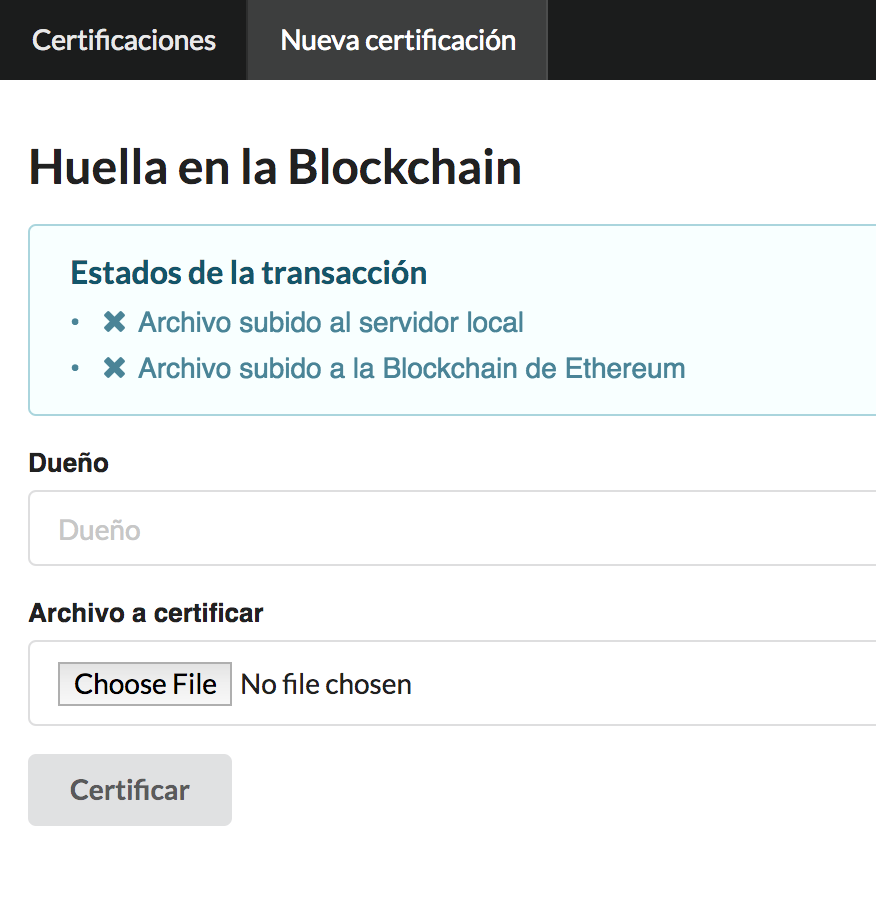
\includegraphics[height=13cm, width=13cm]{alta_certificacion_inicial_sys.png}
  \centering
  \caption{Formulario para dar de alta una certificación}
  \label{fig:alta-certificacion-inicial-sys}
\end{figure}

Aparte de los campos descriptos en el párrafo anterior, se puede ver en la parte superior del formulario un cartel con la leyenda ``Estados de la transacción''. Esencialmente, la transacción dentro del sistema presenta dos estados: el primero en el cual el archivo es transferido al servidor de archivos. A modo de ejemplo, se puede ver en la siguiente imagen:

\begin{figure}[H]
  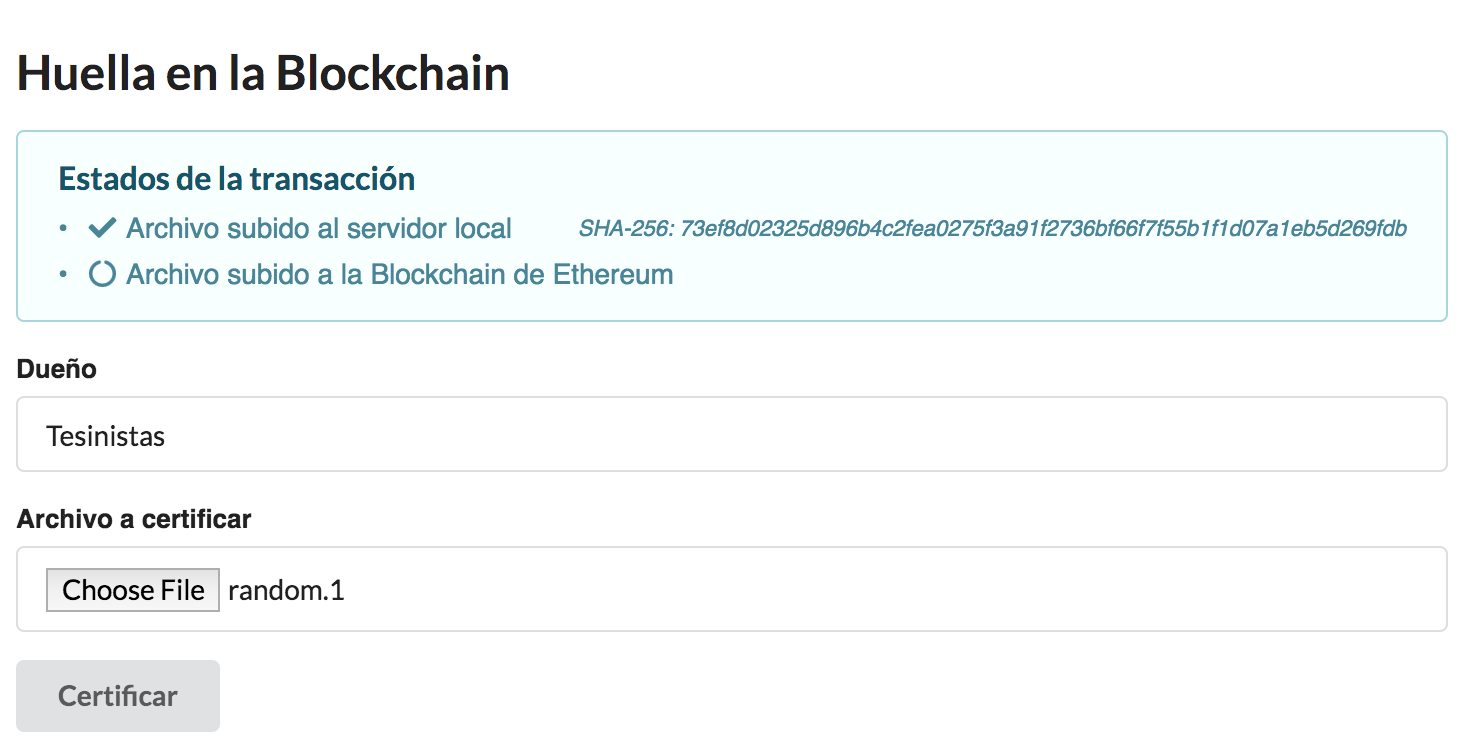
\includegraphics[height=8cm, width=15cm]{alta_certificacion_infs_sys.png}
  \centering
  \caption{Fase 1 completada o transacción en estado 1}
  \label{fig:alta-certificacion-infs-sys}
\end{figure}

Como el propietario ``Tesinistas'' intenta certificar el archivo ``random.1'' y a continuación -tras haber hecho click en el botón ``Certificar''- se puede constatar que las huellas digitales calculadas tanto por el servidor anteriormente nombrado como por la aplicación cliente coinciden, al mismo tiempo que se informa en pantalla. En caso de no coincidir, se informa el problema y se cancela la operación. Con este paso finaliza la fase 1 de la transacción.

Luego, la transacción continua hacia el segundo estado o fase en donde se ejecuta la operación del contrato en la blockchain de Ethereum que tiene como propósito resguardar y difundir el acto certificatorio a través de toda la red. Dado que se necesita hacer uso de una operación de escritura sobre la blockchain de Ethereum (ver \ref{bc_ethereum_smart_contracts}) es necesario realizar el pago correspondiente por el costo de dicha operación, es decir, el costo de ejecutar y registrar en una transacción dentro de dicha red los datos correspondientes a la certificación que se está intentando realizar. Para esta situación, automáticamente se va a desplegar una ventana del plugin \textit{Metamask} para poder autorizar una transferencia de criptomonedas desde la cuenta que solicita la certificación hacia la blockchain. A continuación se mostrará una imagen de ejemplo:

\begin{figure}[H]
  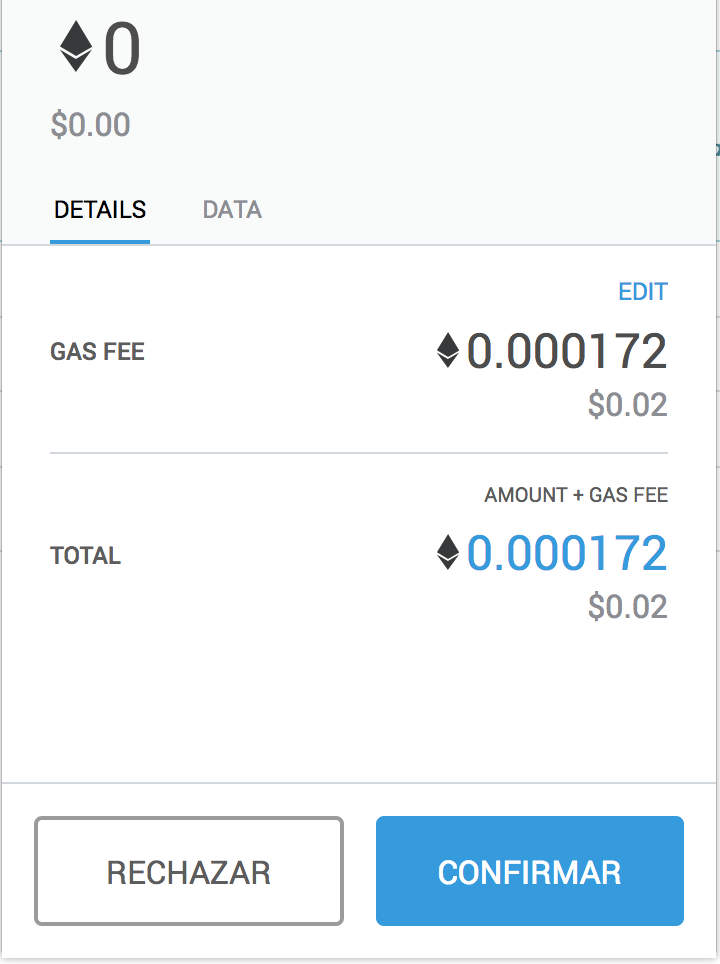
\includegraphics[height=12cm, width=8cm]{alta_certificacion_metamask_sys.png}
  \centering
  \caption{Ventana de Metamask para autorizar la transacción en la blockchain}
  \label{fig:alta-certificacion-metamask-sys}
\end{figure}

Ninguna de las operaciones del contrato implementado para este trabajo cobra un adicional diferenciado por el uso del servicio (recordar \ref{bc_ethereum_smart_contracts}), en cambio, lo que sí se cobra, y es obligatorio siempre, es el \textit{gas} requerido para la realización de la transacción en la blockchain, tal como se explicó en [ref. Gas en Ethereum]. Esta información se puede ver reflejada en imagen expuesta anteriormente es donde se ve, a partir de los datos recabados por Metamask, que el arancel de la operación es 0 mientras que la tasa del \textit{gas} es una fracción de Ether, la moneda usada dentro de Ethereum.

Al confirmar esta transacción, se tendrá que esperar unos momentos -en el orden de algunos minutos- a que la misma se concilie, se difunda y se asiente por varios de los nodos de la red blockchain (muy similar a lo descrito en \ref{bc_bitcoin_net_overview} y \ref{bc_bitcoin_security}) y, finalmente, si todo sucede exitosamente, entonces la operación quedará definitivamente confirmada, a saber:

\begin{figure}[H]
  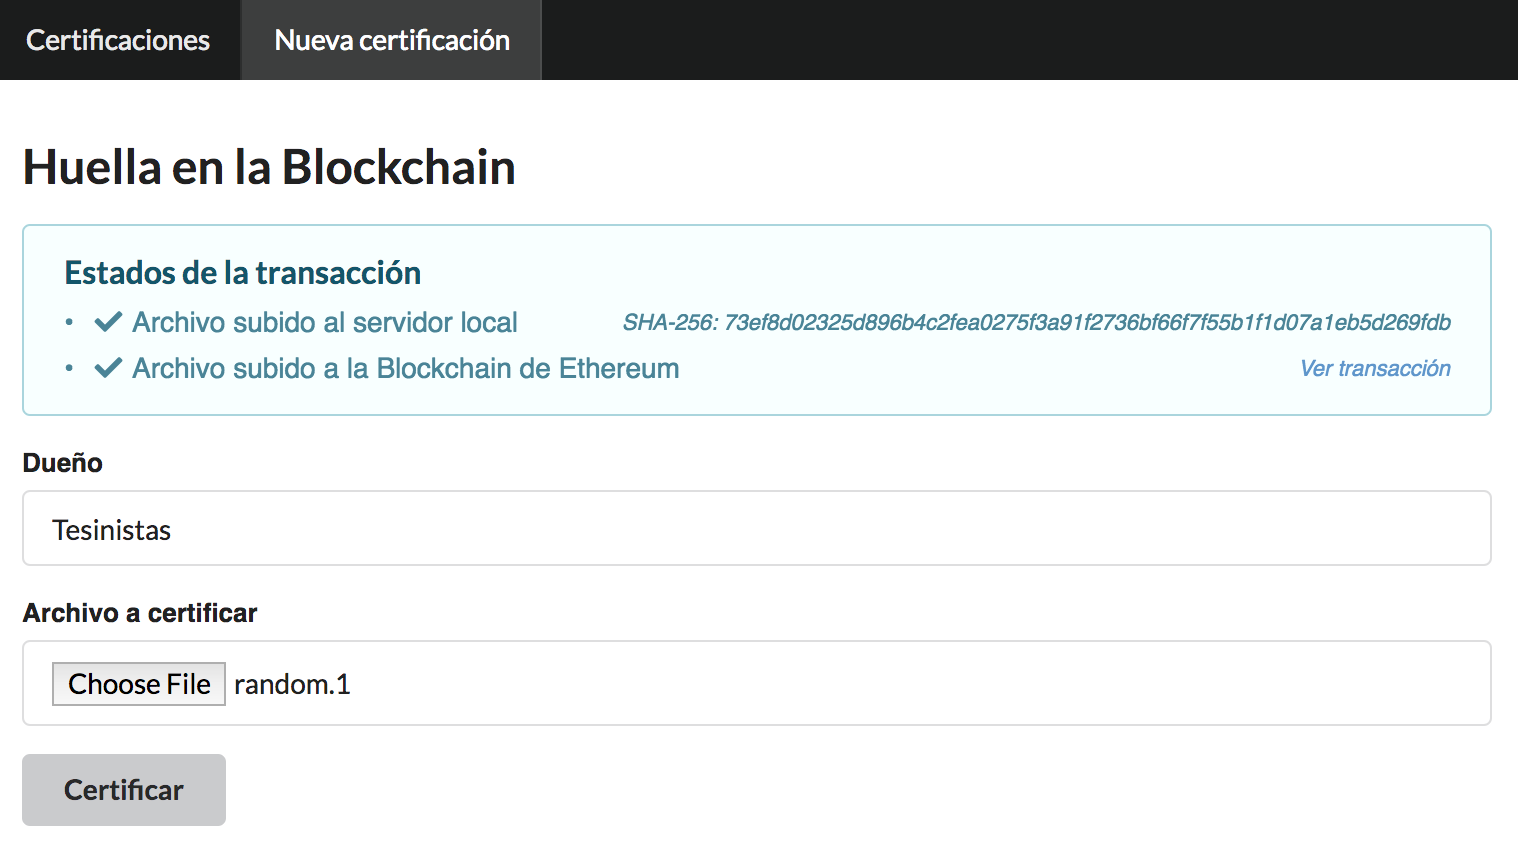
\includegraphics[height=8cm, width=13cm]{alta_certificacion_final_sys.png}
  \centering
  \caption{Transacción registrada en la blockchain y operación completa}
  \label{fig:alta-certificacion-final-sys}
\end{figure}

En la imagen hay un enlace para poder ver el detalle de la transacción registrada por fuera de este sistema, y se explicará con más detalles en la sección \ref{transacciones_blockchain_provider_publico}.

Con el objeto de entender algunos detalles adicionales, a continuación, se introducirá el código que encapsula toda la lógica anteriormente descripta:

\begin{minipage}{\linewidth}
\begin{lstlisting}[frame=single, belowskip=1em, aboveskip=2em,  language=javascript, captionpos=b, caption=Código de alta de certificación, label={lst:alta_certificacion}]
  const file  = this.uploadInput.files[0]
  const owner = this.ownerInput.value
  const data  = new FormData();
  data.append('file', file);
  // Starting upload process to file server
  this.setState({ fileUploadLocalServerStatus: 'pending' })
  calculateDigest(file)
    .then(digestFromClient => {
      axios.post(config.fileserver.endpoint, data)
        .then((response) => {
          const { digest: digestFromServer, file } = response.data
          if (digestFromServer === digestFromClient) {
            this.setState({ digest: digestFromClient, fileUploadLocalServerStatus: 'done' })
            // Listen to blockchain event
            CertContractApi.once('FileAdded', (error, postData) => {
              if (!error) {
                this.setState({ fileUploadEthereumblockchainStatus: 'done', txHash: postData.transactionHash })
              } else {
                console.error('Fallo algo en la subida a la blockchain de Ethereum')
              }
            })
            // Call the contract
            const prefix = '0x' + digestFromClient
            this.setState({ fileUploadEthereumblockchainStatus: 'pending' })
            CertContractApi.addFile(prefix, owner, file)
          } else {
            console.error('Error! Digest cliente != digest servidor')
          }
        })
    })
\end{lstlisting}
\end{minipage}

Lo primero que transcurre, entre las líneas 1-4, es la obtención de los datos del formulario. A partir de la línea 5 comienza a subirse el archivo al servidor de archivos: en 6 se señaliza que esta operación se encuentra pendiente (esto da comienzo a la fase 1 anteriormente descripta). En la línea 7 se procede a calcular la huella digital del archivo dispuesto en el formulario, es decir, en la aplicación cliente, haciendo uso de promesas\footnote{Una promesa es una estructura que permite secuenciar cómputos de naturaleza asincrónica con el objeto de facilitar la lectura del código}. Luego de obtener la huella, se realiza la conexión remota contra el servidor de archivos (linea 9) cuyo funcionamiento fue detallado en \ref{detalles_servidor_archivos}. Si todo transcurre exitosamente, entonces, como se puede ver en la línea 11, se recibirá como respuesta la huella digital calculada por el servidor y la URL del archivo. En 12 se comparan ambas huellas: si no son iguales, se informa el error y se cancela la operación; en caso de ser iguales, se señaliza el fin de la subida del archivo -fase 1- en la línea 13.
En la línea 15 se registra un manejador para un evento. Esto es una práctica común en Javascript y en Node.JS dado que buena parte del desarrollo en estas tecnologías están orientadas a eventos y procesamiento que ocurre asincrónicamente y, consecuentemente, esto favorece el rendimiento (ver, por ejemplo, \cite{TilkovVinoski2010}). En este caso particular, es prácticamente menester usar un mecanismo asincrónico porque la interacción con la blockchain es relativamente muy lenta, y así se evita retrasar el resto de las funcionalidades de la aplicación. El evento particular, para este código que se está describiendo, es \textit{FileAdded}, el cual se dispara cuando la transacción en la blockchain se completa, ya sea exitosamente o con errores. Sea cual sea el caso, cuando el evento se genera, se ejecuta la función asociada a él en donde se puede ver, en la línea 17, que se vuelve a hacer uso de la señalización para cambiar el estado de la operación -marcando el fin de la fase 2- y, con esto, dar fin a la operación.
Luego de registrar el evento, el último paso es realizar el llamado asincrónico a la operación de agregar el archivo en la blockchain (línea 25). Cabe destacar que tanto aquí, como en el registro del evento, se hace uso de un módulo llamado \textit{CertContractApi} el cual abstrae y separa toda la interacción contra la blockchain mediante la librería Web3 (de hecho, en ninguna de las operaciones se ve su uso por si en un futuro se decide cambiar la librería que provee las facilidades para comunicarse con la blockchain de Ethereum)

\subsubsection{Operación de listar certificaciones (\textit{frontend})}

Otra de las grandes funcionalidades que ofrece el sistema es la posibilidad de ver el listado de las transacciones ejecutadas junto a una verificación sobre el estado de inmutabilidad de los archivos asociados. En la sección \ref{listado_certificaciones} ya se repasó a alto nivel el flujo y las interacciones que intervienen en este requerimiento. A partir de ahora, se hará una explicación más detallada mostrando código e imágenes de esta operación

\begin{figure}[H]
  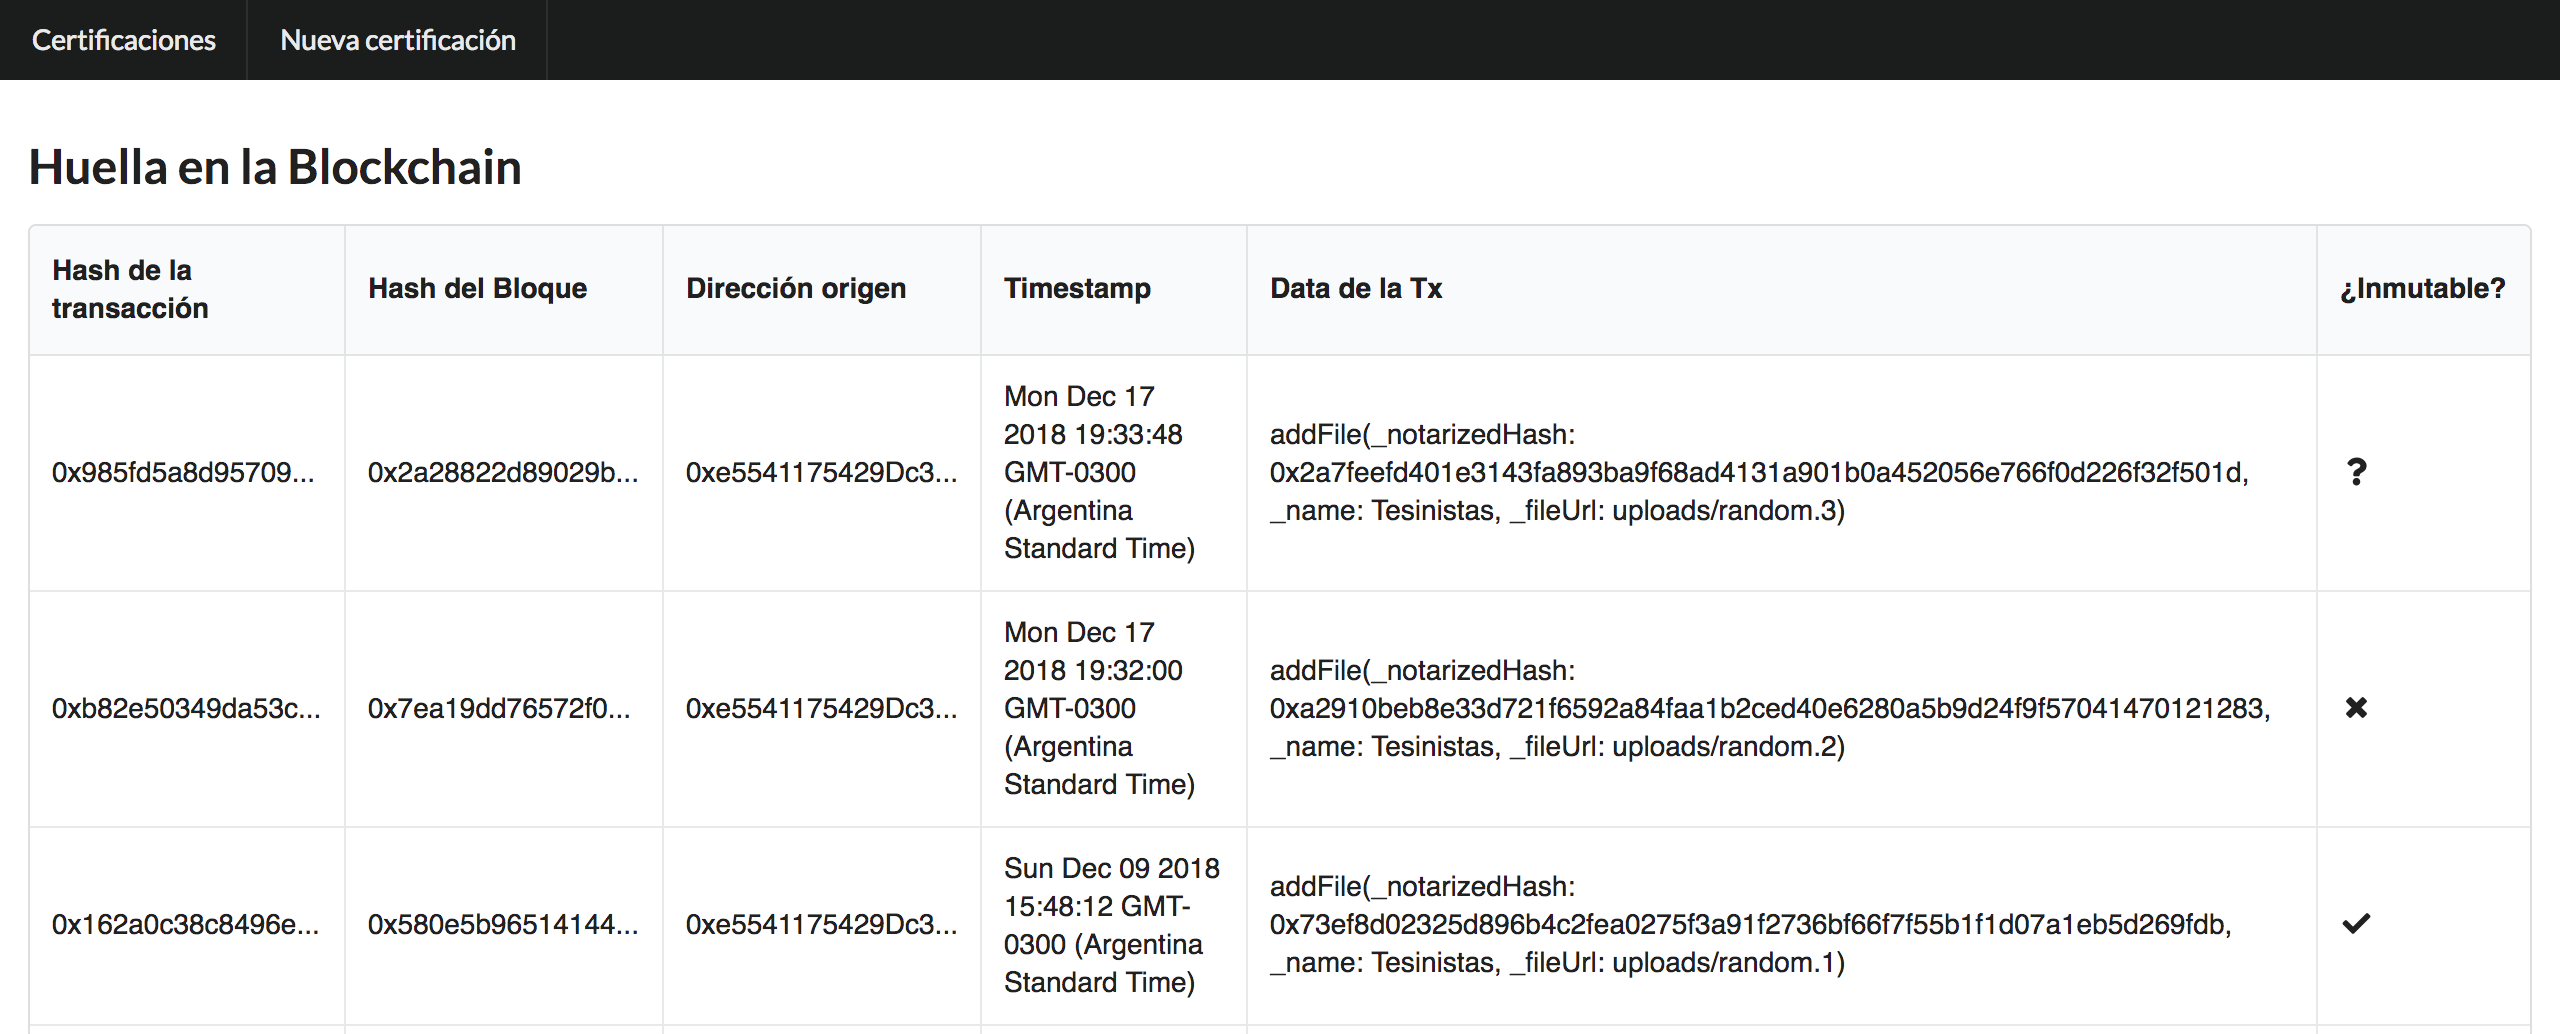
\includegraphics[height=6cm, width=13cm]{listado_certificaciones_ej.png}
  \centering
  \caption{Ejemplo de listado de certificaciones}
  \label{fig:listado-certificaciones}
\end{figure}

Como se puede ver en la imagen anterior, lo que se muestra son las últimas tres transacciones realizadas en el sistema. Cabe destacar en este punto que las transacciones listadas en esta vista provienen directamente de la blockchain, con lo cual, todos los datos -excepto los ``datos propios''- son extraídos exclusivamente de los metadatos de las transacciones guardadas en dicha base de datos. De cada una se puede ver la siguiente información:

\begin{itemize}
  \item \textbf{Hash de la transacción:} constituye la huella digital de una transacción. Permite identificarla unívocamente entre todas las transacciones almacenadas en la blockchain.
  \item \textbf{Hash del bloque:} constituye la huella digital de un bloque, el cual, como ya se ha explicado en \ref{bc_bitcoin_block} y en \ref{bc_ethereum_data_layer}, contiene un paquete de transacciones.
  \item \textbf{Dirección de origen:} representa la dirección de la cuenta desde donde se ha solicitado y aprobado la operación para certificar un archivo. Desde la misma se realiza el pago correspondiente al servicio y al gas insumido para poder efectuarla.
  \item \textbf{\textit{Timestamp} (Fecha y hora de la transacción):} es en realidad la fecha y la hora del momento en el cual se firma el bloque que contiene a la transacción relacionada; por lo tanto, puede haber un desfasaje entre la fecha y hora real en la cual se genera la certificación con respecto a este \textit{timestamp} que proviene del bloque mencionado. Si se desea mayor precisión, se podría incluir como dato adicional dentro de los ``datos propios'' de la transacción, tal como se explicó en el apartado \ref{datos_guardar_blockchain}.
  \item \textbf{Datos propios de la transacción:} Son los datos del dominio propio de la aplicación. En concreto, el \textit{\_notarizedHash} es la huella digital calculada para el archivo certificado, el \textit{\_name} es el nombre del propietario de la acción y el \textit{\_fileUrl} es la locación del archivo a certificar. Recordar que las decisiones sobre la selección de estos datos fue discutida en \ref{datos_guardar_blockchain}.
  \item \textbf{Estado de inmutabilidad del archivo:} Por último, en esta columna se muestra la verificación de integridad de los archivos que se realiza en el momento inmediatamente posterior a la recuperación de las transacciones desde la blockchain de Ethereum. Hay tres estados que serían los siguientes:
  \begin{itemize}
    \item Archivo perdido (signo de pregunta): Significa que en la certificación asociada se ha perdido el archivo o por alguna otra razón fue imposible leerlo. Por ejemplo, en la imagen previa se puede ver que la última transacción (la primera de la tabla) se encuentra en este estado puesto que deliberadamente se ha borrado el archivo en el sistema de archivos del servidor que lo alojaba.
    \item Sin cambios (tilde bien): Significa que en la certificación asociada, el archivo se encuentra intacto, sin ninguna modificación desde el momento en el cual se gestionó la operación. Es el caso de la anteúltima certificación que se ve en la imagen previa.
    \item Con cambios (tilde cruz): Significa que el archivo sufrió alguna clase de modificación y, por tanto, no se puede confiar en su contenido. De la figura \ref{fig:listado-certificaciones} se puede observar que la antepenúltima certificación está en tal estado, puesto que deliberadamente se ha alterado el contenido del archivo relacionado, con lo cual, la huella digital calculada sobre él es distinta a la previamente registrada en la blockchain.
  \end{itemize}
\end{itemize}

Para entender con mayores detalles cómo se solicitan estos datos, a continuación se expondrán la porciones de código involucradas en esta tarea:

\begin{minipage}{\linewidth}
\begin{lstlisting}[frame=single, belowskip=1em, aboveskip=2em,  language=javascript, captionpos=b, caption=Inicialización del listado de transacciones, label={lst:inicio_listado_transacciones}]
  componentDidMount() {
    CertContractApi.getTransactions('FileAdded').then(transactions => {
      transactions = transactions.sort((t1, t2) => {
        return (t2.block.timestamp - t1.block.timestamp)
      })
      this.setState({
        blockchainInfo: 'ready',
        txs: transactions
      })
      transactions.forEach(this.calculateDataChanges)
    })
  }
\end{lstlisting}
\end{minipage}

El fragmento de código correspondiente en \ref{lst:inicio_listado_transacciones} muestra lo que sucede cuando el listado se inicializa (\textit{componentDidMount} es el método en React que se encarga de esto, ver más detalles en \cite{React2018}). Comienza solicitando todas las transacciones del contrato desplegado en la blockchain vinculadas al event \textit{FileAdded} descrito previamente en \ref{operacion_alta_certificacion} y una vez recuperadas se orden según el \textit{timestamp} de cada una (línea 3), luego se señaliza en la aplicación que las transacciones están listas para ser mostradas (línea 6) y finalmente, para cada una de estas certificaciones, se procede a realizarse la verificación de la huella digital.

Los detalles acerca de cómo se realiza la verificación se explicaran a continuación:

\begin{minipage}{\linewidth}
\begin{lstlisting}[frame=single, belowskip=1em, aboveskip=2em,  language=javascript, captionpos=b, caption=Verificación de la huella digital en las transacciones, label={lst:verificacion_huella_transaccion}]
  calculateDataChanges(tx) {
    const notarizedHash = this.notarizedHashFromTx(tx)
    const filePath      = this.filePathFromTx(tx)

    fetch(`${config.fileserver.endpoint}/${filePath}`)
      .then(calculateDigestFromResponse)
      .then(digest => {
        if (notarizedHash === `0x${digest}`) {
          this.setState((oldState, props) => {
            return { txChanges: { ...oldState.txChanges, [notarizedHash]: 'unchanged' } }
          })
        } else {
          this.setState((oldState, props) => {
            return { txChanges: { ...oldState.txChanges, [notarizedHash]: 'changed' } }
          })
        }
      })
      .catch(() => {
        this.setState((oldState, props) => {
          return { txChanges: { ...oldState.txChanges, [notarizedHash]: 'notfound' } }
        })
      })
  }
\end{lstlisting}
\end{minipage}

Dada una transacción, el primer paso es extraer de ella la huella digital y la ubicación del recurso (archivo) registrados al momento de darse de alta la certificación; esto se hace en las líneas 2 y 3, respectivamente. Con dicha \textit{URI} se solicita al \textit{endpoint} del servidor de archivos el archivo asociado a la transacción (línea 5) y tras su recuperación se calcula su huella digital (línea 6). En la línea 8, si la comparación entre la huella almacenada en la certificación coincide con la calculada en este momento, entonces se señaliza a la aplicación para que la transacción actual se marque como ``sin cambios'' (línea 9); en caso contrario, se marcará como ``con cambios'' (línea 13). Si hay algún tipo de problema, como por ejemplo, una falla de lectura en el archivo, la función \textit{catch} se ejecutará y se encargará de señalizar la aplicación para que la transacción se marque como ``archivo perdido''.

\subsection{Transacciones de la blockchain desde un \textit{provider} público (\textit{backend})}
\label{transacciones_blockchain_provider_publico}

Luego de analizar las funcionalidades que ofrece la aplicación, es decir, las capacidades de certificar y mostrar las certificaciones, alguien podría preguntar: ¿y cómo puedo confiar en los datos que circulan dentro de la aplicación? Pues bien, tal como sucede en una aplicación convencional en donde la información se almacena en un repositorio o en una base de datos a la cual cualquiera (despreciando cualquier mecanismo de permisos) puede acceder de manera independiente para verificar esa información, análogamente es posible realizar este chequeo conectándose a la blockchain por medio de un canal o servicio conocido como \textit{provider}. La clara ventaja de esto, como ya se ha señalado en las secciones \ref{bc_bitcoin_security} y \ref{bc_bitcoin_net_overview}, es que, por un lado, al tratarse de una base de datos inmutable se tendrá la seguridad de que las transacciones que se verán allí no podrán ser alteradas jamás y, por otro lado, al ser una base de datos distribuida conformada por múltiples nodos, esto da la garantía de poder acceder a cualesquiera de ellos de forma indistinta y poder ver el mismo conjunto de datos, teniendo mejor disponibilidad y respaldo frente a una base de datos tradicional que tiende a ser centralizada.

En síntesis, frente a una situación en la cual no se pueda confiar en la aplicación, si se tuviera un repositorio de datos centralizado o semi-centralizado, el mismo sería mucho más vulnerable a sufrir alteraciones en sus datos, y por consiguiente, pérdida de confianza en los mismos, que, en cambio, disponer de una blockchain que ofrece mayores seguridades en cuanto a la inmutabilidad, la disponibilidad y la transparencia de la información.

Tal como se ha aclarado recién, un \textit{provider} es un medio o herramienta conectada a algún nodo conformante de la blockchain que permite examinar los bloques y las transacciones registradas.

Para este trabajo, se ha usado la herramienta \textit{Etherscan} que es un explorador de bloques de redes de tipo Ethereum \cite{Etherscan2018}. A través de esta utilidad es posible ver todas las trazas y las conexiones entre los distintos bloques y transacciones, a través de las direcciones asociadas a cuentas convencionales, o bien, contratos. Este último es de especial importancia para este desarrollo, puesto que hay una sección especial en donde se puede ver qué transacciones se hicieron hacia un contrato en particular y, entre otra información, los eventos que disparó el mismo.

Por ejemplo, para el contrato particular del trabajo, se pueden ver estas últimas transacciones

\begin{figure}[H]
  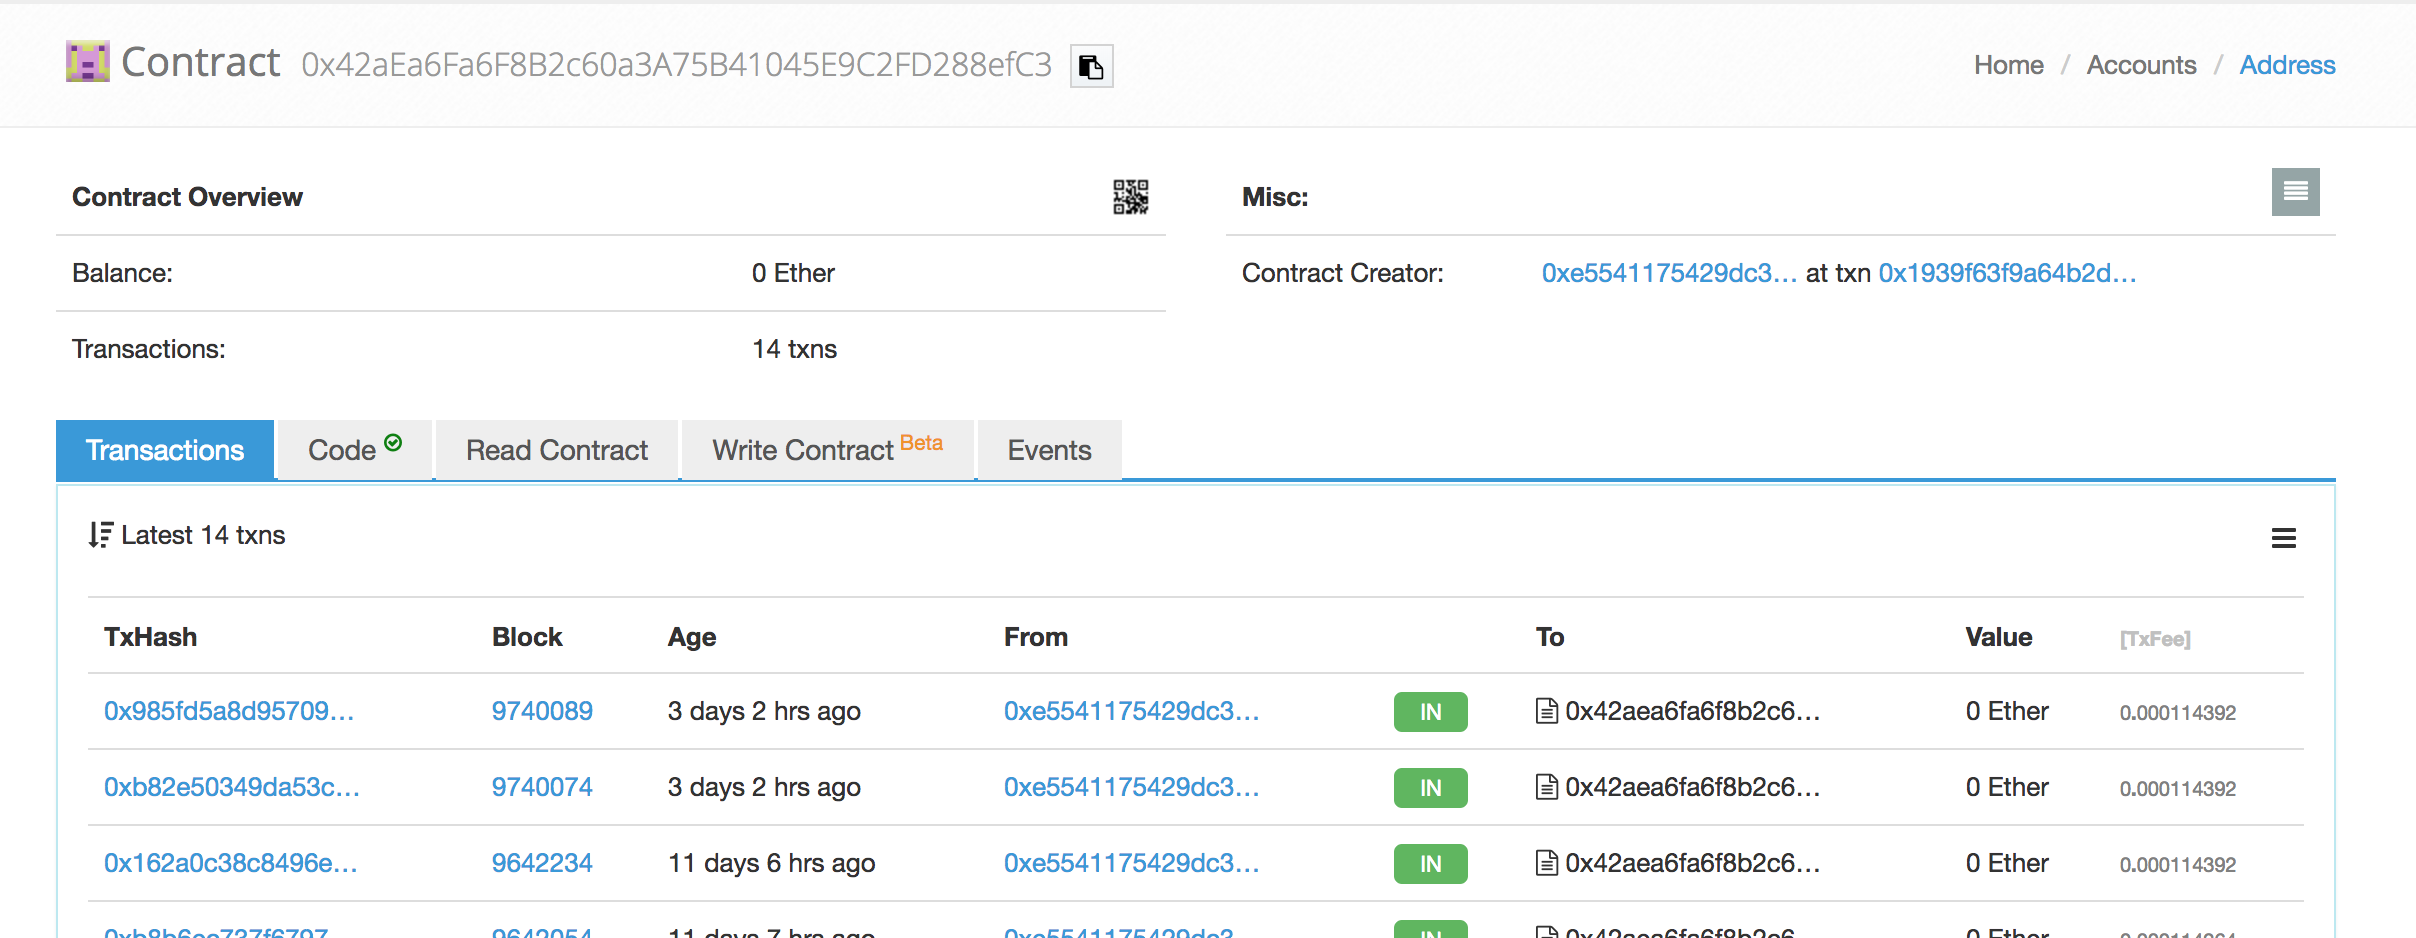
\includegraphics[height=6cm, width=13cm]{etherscan_transacciones.png}
  \centering
  \caption{Transacciones del contrato vistas desde Etherscan}
  \label{fig:etherscan-transacciones}
\end{figure}

Donde, como se puede ver, las últimas tres corresponden a las tres últimas que se vieron en la figura \ref{fig:listado-certificaciones}

En cuanto a los eventos disparados, se tienen los siguientes:

\begin{figure}[H]
  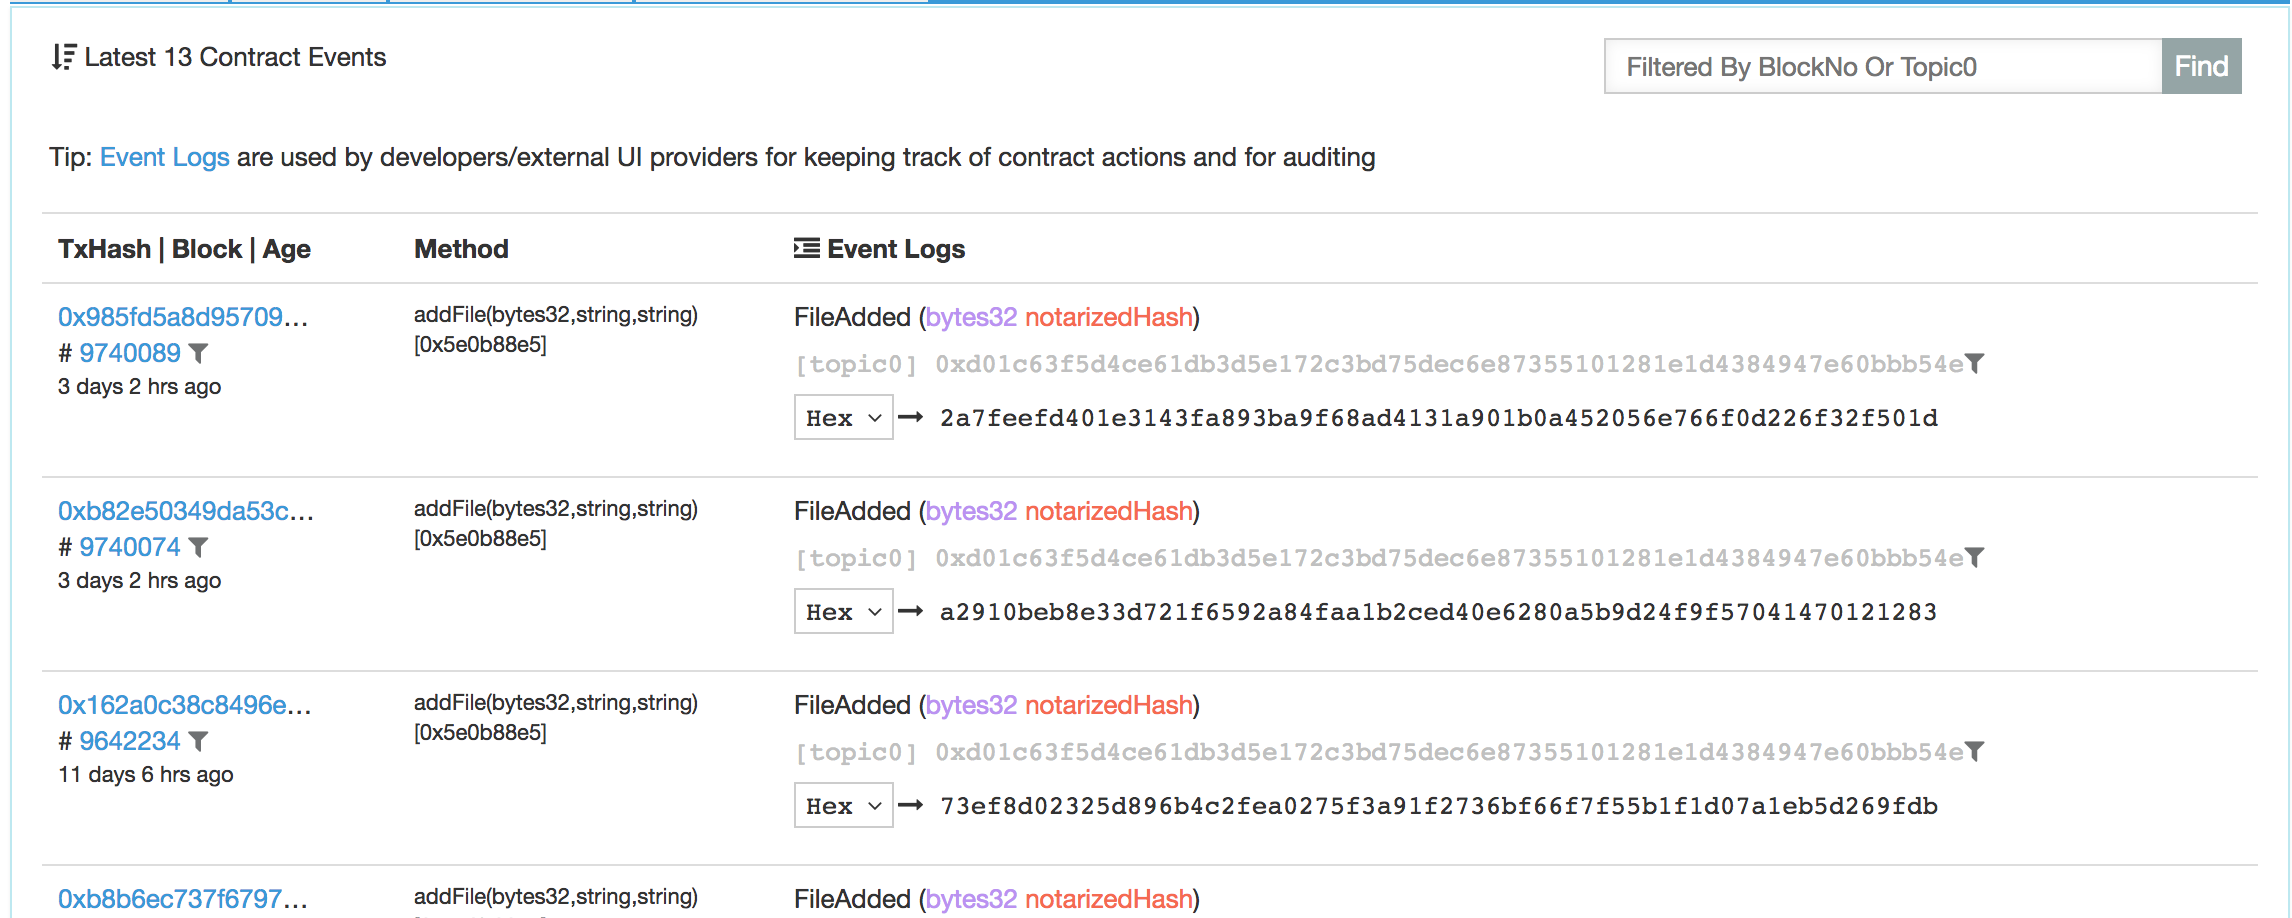
\includegraphics[height=6cm, width=13cm]{etherscan_eventos.png}
  \centering
  \caption{Eventos del contrato vistos desde Etherscan}
  \label{fig:etherscan-eventos}
\end{figure}

Que también se corresponden con las certificaciones vistas en la figura \ref{fig:listado-certificaciones}

En este punto debería quedar claro que la operación de listado confeccionada para la aplicación como parte del \textit{frontend}, es exactamente esto, una \textit{vista} que consume los datos directamente de la blockchain y los muestra de manera similar a como se ha visto en el apartado presente. Cualquiera con acceso a un explorador o un \textit{provider} conectados a la misma red deberán ver la misma información siempre, sin importar a cuál de los nodos elija conectarse.

\subsection{Recapitulación}
\label{recapitulacion_impl_solucion}

En esta sección se ha descrito en detalle las principales funcionalidades que aporta el prototipo del sistema que realiza certificaciones de archivos y usa la blockchain de Ethereum como \textit{backend} descentralizado. El objetivo buscado con esta arquitectura fue el de distribuir y replicar las transacciones con las huellas digitales -generadas desde una aplicación \textit{frontend}-  entre muchos nodos de manera implícita para que la confianza no recaiga en un único punto y, así, brindar mejoras sustanciales en cuanto a la seguridad y a la disponibilidad del servicio.
Se han discutido, en primer lugar, variantes dentro de la propia arquitectura en pos de lograr mayor control propio del mismo, pero sacrificando las bondades de la descentralización. Luego se han puesto en escena las especificaciones de las operaciones soportadas por el prototipo. Posteriormente, se brindaron detalles de la implementación de estas operaciones con gráficos demostrativos. Por último, se han podido explorar las transacciones generadas por la aplicación desde un explorador de la blockchain con el propósito de demostrar que los datos o las certificaciones generadas se pueden ver por fuera del sistema desarrollado y que accediendo a cualquier nodo de esta blockchain se van a visualizar exactamente los mismos datos.

\newpage
\section{Conclusiones}
\label{conclusion}

La presente tesina planteó una interrogante acerca del problema de la comprobación de integridad de archivos sobre redes. En primer lugar, se discutieron los inconvenientes inherentes a la centralización actual de dicha prueba. Luego, se brindó un contexto histórico en torno al surgimiento y a la filosofía de la descentralización, dando lugar a un nuevo escenario para presentar una nueva alternativa de solución a este problema. Tras ello, se desarrolló el marco teórico de blockchain, mostrando sus conceptos originarios para luego explicar las dos implementaciones más grandes y populares: Bitcoin y Ethereum. En la primera se explicaron las ideas fundamentales que son comunes a prácticamente toda blockchain, en particular, las transacciones, los bloques, el funcionamiento de la red y la política de consenso basada en prueba de trabajo. En la segunda se extendieron estas componentes para incluir la posibilidad de realizar cómputo descentralizado por medio de contratos inteligentes, con los cuales, se podrían desarrollar aplicaciones genéricas sobre la blockchain, más allá del uso estrictamente monetario para el cual fue originalmente diseñado Bitcoin. Finalmente, se presentó una arquitectura piloto que describe la solución alterna al problema de la verificación de archivos haciendo uso de los mencionados contratos inteligentes.

Se ha visto como ventajas que la nueva solución provee una fuente de información confiable basada en la inmutabilidad de los datos una vez que son confirmados dentro de la blockchain y accesible desde cualquier nodo conformante de dicha red. A diferencia de las soluciones centralizadas tradicionales, las vías de ataque son drásticamente reducidas dado que no alcanza con alterar maliciosamente o denegar los datos registrados por uno de los nodos, puesto que hay redundancia en todos ellos. Por otra parte, dadas las demoras necesarias para confirmar transacciones por los mecanismos de consenso, en general toda solución basada en blockchain será más lenta. Además, o por lo menos en la implementación realizada en este trabajo, es necesario contar con una billetera y dinero digital para poder realizar las operaciones. En el apartado ``Trabajos futuros'' (\ref{future_works}) se explicarán algunos mecanismos para mitigar estos inconvenientes.

Respecto a las expectativas antes y después de esta investigación, se pueden mencionar:

\begin{enumerate}
  \item Antes de comenzar a recabar y analizar información sobre el consenso en Bitcoin, los tesinistas creían que dicho algoritmo era totalmente tolerante a fallas bizantinas. A medida que se avanzó con esto, se comenzó a ver que la premisa anterior no era del todo verdadera y que dicha tolerancia es parcial. Es decir, a diferencia de otros algoritmos, como por ejemplo PBFT, que demostraron ser completamente tolerantes a fallas bizantinas, los mecanismos de consenso usados en Bitcoin y Ethereum (al día de hoy) -basados en prueba de trabajo-, son probabilísticamente tolerantes a dichas fallas, pero en la práctica han mostrado comportarse muy bien y, además, son anónimos por diseño (en tanto que PBFT no lo es) lo cual es fundamental en implementaciones de blockchains públicas.
  \item Eliminar completamente la centralización es un trabajo mayor del pensado. Por ejemplo, si se analiza el prototipo realizado para esta tesina, la aplicación cliente -frontend- y el servidor de archivos actualmente residen en un servidor centralizado y podrían ser vulnerable a ataques. Asimismo, la conexión del frontend a la blockchain es punto a punto y dicho canal también podría ser atacado. De todas formas, estos problemas son abordables, y en ``Trabajos Futuros'' (\ref{future_works}) se discutirán algunas soluciones.
  \item El desarrollo del prototipo tuvo sus dificultades puesto que las librerías a usar aún están en proceso de desarrollo constante, con lo cual, la interfaz de muchas de ellas es algo inestable. De hecho, se ha contribuido a mejorar algunas de estas herramientas open source.\footnote{\url{https://github.com/ConsenSys/abi-decoder/pull/29}}.
\end{enumerate}

Otra cuestión a destacar es que más allá de las implementaciones vistas de blockchain en este trabajo, existen centenares más, donde cada una busca solucionar un problema específico y concreto. De hecho, existe una extensa clasificación de acuerdo al mecanismo de consenso usado -priorizando uso de energía, tolerancia a ataques, velocidad en cuanto al tiempo promedio en confirmar una transacción y escalabilidad en la red-, a la visibilidad de los datos (si es pública o privada), entre otros. Cada negocio buscará su tipo ideal de blockchain acorde a su dominio.

Asimismo, es interesante mencionar la gran cantidad de líneas de investigación y desarrollo que se pueden derivar del estudio de blockchain. Por ejemplo, se puede innovar en temáticas tales como teoría de lenguajes (para describir contratos inteligentes), máquinas virtuales, probabilidad y estadística (estudio de la robustez de los mecanismos de consenso y resistencia a ataques), criptografía, sistemas distribuidos (protocolos de consenso, en particular) y hasta en aspectos económicos y de mercado que escapan de la computación en sí.

Finalmente, vale destacar que el tema desarrollado en la presente tesina ha sido presentado y aceptado en la WICC San Juan 2019, enmarcado dentro de la línea de investigación de ``Seguridad Informática''.

\newpage
\section{Trabajos futuros}
\label{future_works}

A lo largo del desarrollo de la tesina se formularon distintas interrogantes en cuanto a la estructura arquitectónica de la solución propuesta. Una de ellas particularmente referida a los conocimientos básicos que debe tener el usuario final, como por ejemplo, la noción de conceptos como el gas consumido por las transacciones que se paga en \textit{ether} y el uso de extensiones para la administración de billeteras (Metamask). Una solución para este tipo de problemas es el uso de estaciones de gas. Las estaciones de gas están conformadas por una serie de componentes que realizan el pago y el envío a la red de las transacciones, de una forma transparente para el usuario final. Las componentes y el rol que ocupan cada una de ellas es:

\begin{enumerate}
  \item El usuario final que posee una cuenta con una clave privada que es utilizada para crear las transacciones y firmarlas (la cuenta no posee \textit{ether}).
  \item Distribuidor de transacciones, es la cuenta encargada de encapsular las transacciones de los usuarios finales y enviarlas a un contrato inteligente para luego ser ejecutada. Esta cuenta debe poseer balance en \textit{ether}.
  \item Un contrato inteligente denominado ejecutor, que es el encargado de ejecutar la transacción del usuario, previamente validando su contenido y calculando la cantidad de gas necesaria para ser ejecutada.
  \item Estación de gas, es un contrato inteligente que posee balance en \textit{ether} o algún otro tipo de criptomoneda que son utilizadas para pagarle al distribuidor de transacciones por el envío de la transacción al contrato ejecutor y su distribución en la red.
\end{enumerate}

Entonces la secuencia de pasos sería la siguiente: el usuario final crea y firma la transacción (utilizando su clave privada) y la envía a la cuenta del distribuidor. Este último posee \textit{ether}, por lo tanto, puede ejecutar la función sobre el contrato ejecutor que le permite enviar la transacción del usuario final. Una vez en el contrato ejecutor, la transacción es verificada y enviada a la red, y a su vez éste calcula el gas que utilizó el distribuidor para realizar todo el proceso y se le reembolsa a través del contrato estación de gas.
De esta manera el usuario no necesita instalar ninguna extensión o aplicación extra para el uso de billeteras, ya que la clave privada se podría crear a la hora del registro del usuario y otra ventaja es que no necesita obtener \textit{ether} para la ejecución de las transacciones.

Otra de las problemáticas planteadas fue el poder eliminar completamente la centralización desde el punto de vista de la instalación y despliegue de la aplicación y de la comunicación con la blockchain. En cuanto a lo primero, se destacó que la existencia de una única instancia tanto de aplicación cliente como de servidor de archivos podría ser un punto débil desde la perspectiva de la seguridad y la disponibilidad del servicio. El mismo problema se plantea con la descarga de la aplicación cliente, puesto que se haría desde un repositorio centralizado. Una forma de atacar estos problemas es usando IPFS\cite{Ipfs2019}, el cual está pensado como sistema de archivos distribuido par-a-par. Si las distintas versiones oficiales de la aplicación cliente se alojasen allí, entonces la descarga de las mismas serían mucho más seguras por estar justamente delegando la confianza sobre la red y, por el contrario, que no recaiga en un único punto de acceso. En cuanto a lo segundo, la comunicación a los nodos, lo ideal es tener un conjunto de nodos totalmente sincronizados y estables, de forma tal que las peticiones o envío de información a la blockchain sean alternados y no dejar de prestar servicio si uno de los nodos se cae, otorgando alta disponibilidad al sistema. Para la solución propuesta en la tesina se utilizó un solo proveedor de acceso, Infura, que brinda una URL de conexión para enviar y recibir los mensajes RPC-JSON. Éste es un servicio gratuito y no es dedicado, por lo que el flujo de entrada y de salida es un tanto congestionado. Mantener varios nodos con la blockchain sincronizados es muy costoso: al momento de escribir la tesina la base de datos de Ethereum pesa alrededor de 224.15 GB. Existen alternativas como QuikNode\cite{Quiknode2019} o Infura en su versión paga, que proveen el acceso a un nodo totalmente sincronizado y dedicado, lo cual es una buena alternativa a la creación de uno propio.

Otro caso de uso que se podría implementar para un trabajo futuro, es la creación de una aplicación descentralizada que certifique y realice el seguimiento de los títulos universitarios dentro de una blockchain pública, o bien, dentro de una privada. Las blockchains privadas son altamente performantes en cuanto a velocidad y costos, donde el precio del gas utilizado para ejecutar las transacciones es muy bajo o incluso, en ciertos casos, nulo.
Las blockchains privadas poseen una forma de gobernanza distinta a las públicas ya que las decisiones de cambios o modificaciones de protocolo se realizan mediante el voto de las partes involucradas. La información que reside dentro de este tipo de blockchains es de acceso público, lo que es privado es el derecho a formar parte de la red mediante la inclusión de un nuevo nodo. Un ejemplo de este tipos de redes es el de la Blockchain Federada Argentina\cite{Bfa2019}, la cual propone una red en la cual distintas instituciones como  gobiernos provinciales, administración pública y instituciones académicas, entre otros, puedan interactuar entre sí e intercambiar información de una manera sencilla y eficiente. Volviendo al caso de uso propuesto, sería interesante implementar dicha aplicación en una blockchain como la anteriormente descrita, ya que reduciría el costo administrativo y los procedimientos burocráticos que requiere la certificación y verificación de los títulos universitarios.

En el caso que dicha implementación crezca, posteriormente se podría solucionar la interacción con otras blockchains similares -por ejemplo, certificaciones a nivel mundial o en distintas regiones del pais- mediante sidechains\cite{Sidechain2019}, el cual es un mecanismo relativamente nuevo para ``traducir'' o establecer alguna clase de equivalencia desde una red hacia otra. Para el caso previamente planteado, esto podría servir para la legalización de títulos extranjeros: una certificación en la blockchain local podría estar vinculada de alguna manera a otra certificación proveniente de una blockchain extranjera y, a través de este enlace, establecer la legalización del título.


% --- BIBLIOGRAFIA ---

\newpage
\addcontentsline{toc}{section}{Referencias}
\bibliographystyle{unsrtnat}
\bibliography{tesina}

\end{document}
